\documentclass[12pt,a4paper]{report}
\usepackage[utf8]{inputenc}
\usepackage[T1]{fontenc}
\usepackage{lmodern}
\usepackage{geometry}
\usepackage{setspace}
\usepackage{amsmath}
\usepackage{amsfonts}
\usepackage{amssymb}
\usepackage{graphicx}
\graphicspath{{../images/}{./}}
\usepackage[colorlinks=true,linkcolor=blue,citecolor=blue,urlcolor=blue]{hyperref}
\usepackage[numbers]{natbib}
\usepackage{booktabs}
\usepackage{array}
\usepackage{longtable}
\usepackage{multirow}
\usepackage{pdflscape}
\usepackage{adjustbox}
\usepackage{tabularx}

\newcolumntype{Y}{>{\centering\arraybackslash}X}

% Set page margins
\geometry{left=2.5cm,right=2.5cm,top=2.5cm,bottom=2.5cm}

% Set line spacing
\onehalfspacing

\title{Intent-Driven Dynamic Chunking (IDC):\\Segmenting Documents to Reflect Predicted Information Needs}
\author{Christos Koutsiaris\\
Student Number: 24220094\\
Supervisor: Martin J. Hayes\\
\\
University of Limerick\\
Department of Computer Science and Information Systems\\
MSc in Artificial Intelligence}
\date{06/06/2026}

\begin{document}

% Title page
\maketitle


\newpage

% Abstract
\begin{abstract}
Document chunking is a common preprocessing step in retrieval systems that use large language models. Many current approaches split text by fixed token windows, paragraph boundaries, or local semantic coherence. These choices keep processing simple, but they do not ask what information a user is likely to request. This thesis proposes Intent-Driven Dynamic Chunking (IDC), a segmentation method that first predicts plausible user questions for a document and then chooses chunk boundaries so that each segment is likely to answer one of those questions. The intended result is a set of retrievable passages whose boundaries are shaped by anticipated information needs rather than by document length alone.

IDC was implemented and evaluated on six question-answering datasets. Compared with fixed-length windows, sliding windows, coherence-based segmentation, and original paragraphs, IDC obtained the best top-1 retrieval score on four of the six datasets and tied the strongest baseline on the other two, while also achieving the best Recall@5 and Mean Reciprocal Rank on five of the six. The observed top-1 gains over the strongest baseline ranged from approximately 5\% to 67\%, depending on the dataset. The strongest results were obtained when IDC used per-document intent generation and validation-based parameter tuning. These findings suggest that predicted queries can be used not only to expand documents, as in previous retrieval work, but also to decide how documents should be segmented for retrieval-augmented question answering.

\textbf{Keywords:} Document Segmentation, User Intent, Intent-Driven Dynamic Chunking, Information Retrieval, Question Answering, Large Language Models
\end{abstract}

\newpage

% Plagiarism Declaration
\section*{Plagiarism declaration}
I confirm that this master's thesis is entirely my own work, and that all sources and materials used in this thesis are properly referenced and acknowledged. I acknowledge that any form of plagiarism or academic dishonesty is a serious offence and can result in severe consequences, including the revocation of my degree. By signing this declaration, I confirm that I understand the seriousness of these issues and have taken all necessary steps to avoid any act of plagiarism.

\newpage

% Acknowledgements
\section*{Acknowledgements}

To my wife Maria, and to our boys Alexandros and Markos: thank you. The hours that went into this thesis were hours taken from you, and you gave them up with patience, encouragement, and love. This work is as much yours as it is mine.

\newpage

% Table of contents
\tableofcontents

\newpage

% Include the chapter content
\chapter{Introduction}

\section{Motivation and industrial relevance}
Long-document retrieval depends heavily on how the source text is divided before indexing. Search engines, question-answering systems, and retrieval-augmented generation (RAG) pipelines usually retrieve passages rather than whole documents, so the chunk boundary determines what evidence the system can return. In many implementations, however, chunking is still treated as a simple preprocessing rule, such as splitting after a fixed number of tokens. This thesis treats chunking as part of the retrieval model itself: the boundary should be chosen with the likely information need in mind, not only with the document length or context-window limit in mind.

\subsection{Fixed-length chunking}
The simplest and still most common approach is to divide text into uniform chunks of a certain length (for instance, a fixed number of tokens or characters). This strategy is popular because it is straightforward and guarantees each segment stays within an LLM's context window. Yet fixed-length chunking often ignores the text's logical structure. Boundaries are set arbitrarily, sometimes even cutting through the middle of a sentence or topic, which separates context from content. If the fixed chunk size is too large, a segment may include extra, irrelevant text that dilutes its focus; if it is too small, a single coherent passage or answer can be fragmented across multiple chunks. Answer-bearing information can therefore be "lost" in the wrong segment or split between segments, making it harder for retrieval algorithms to locate a direct answer and for an LLM to interpret the content in isolation. Fixed segmentation is also highly sensitive to the chosen segment length: if the length is not tuned well, retrieval quality drops off markedly. This fragility is problematic in real-world settings where documents vary in length and detail. A "one-size-fits-all" slicing of text is not optimal.

\subsection{Coherence-based chunking}
In response, researchers developed segmentation techniques that respect a document's natural structure. Classic algorithms like TextTiling (Hearst, 1997) and C99 (Choi, 2000) introduced the idea of segmenting at topic shifts rather than at fixed intervals. These methods analyze lexical cohesion (how words repeat or cluster) to detect boundaries where the subject matter changes. For example, TextTiling computes similarity between adjacent blocks and looks for "valleys" (low similarity points) that likely indicate a topic change, while C99 clusters sentences based on semantic similarity to group contiguous sentences into topical segments. The resulting chunks usually correspond to natural paragraphs or subtopics, keeping related ideas together. Subsequent research introduced probabilistic topic models (e.g., Latent Dirichlet Allocation) and, more recently, neural transformers trained to predict segment boundaries, all aiming to better capture a document's intrinsic structure. Coherence-based segmentation offers tangible benefits. It often yields more stable retrieval performance across different chunk sizes; keeping each text segment self-contained on one subject allows chunks to be longer without introducing irrelevant content, which benefits both indexing and retrieval. Studies also suggest that content-driven segmentation can help users locate information more easily. These observations show that how we chunk a document truly matters: coherent, meaningful segments tend to serve information needs better than arbitrary splits.

\subsection{Ignoring user intent}
A further gap remains. Nearly all existing chunking techniques, whether simple or sophisticated, focus on a document's internal signals (lexical or semantic cohesion) and largely ignore what the user is actually looking for. They implicitly assume that if we carve the text into logically complete units, a user will be able to find the piece they need. In practice, this assumption often falls short. A segment might be perfectly coherent on a broad topic, yet a user's query could be about a very specific detail within that segment; from the user's perspective, the rest is noise. Conversely, a user's information need might span content that the algorithm has split into two separate coherent segments, leaving the answer divided and harder to retrieve. In essence, traditional segmentation optimizes for the document's structure, not the user's intent. This observation motivates Intent-Driven Dynamic Chunking (IDC): the segmentation should follow the way people actually seek information. Instead of slicing text blindly or purely by topical boundaries, IDC proposes to segment text based on predicted user intent, essentially chunking documents in anticipation of the questions users are likely to ask.

\subsection{Real-world example (SAP documentation)}
The motivation for intent-aware chunking also came from practical work on semantic search for SAP Fiori technical documentation. This material contains long manuals and knowledge-base entries that engineers search with narrow, domain-specific questions, such as "How do I use API X in SAP Fiori elements?" or "What does error code Y mean in this upgrade log?". Fixed token-based splitting often returned a passage with the right keyword but too much unrelated material. In other cases, a relevant sentence was divided across two chunks, so neither retrieved passage contained the full answer. Section-based or coherence-based splitting helped, but it could still return an entire conceptual section when the engineer needed one operational detail.

Because of this disconnect between how documents were segmented and the questions users asked, search became inefficient. Engineers often had to open multiple results or read through extraneous text to find their answer. Sometimes relevant information was overlooked because it was buried inside an overly large chunk or split across chunks such that each piece seemed irrelevant in isolation. This misfit affects search accuracy and degrades the quality of AI-driven dialogues or summaries that rely on retrieved chunks; irrelevant content can confuse generative models, leading to inaccurate or overly verbose answers. This creates a practical incentive to improve chunking. Companies like SAP (and, more generally, any organization with large knowledge bases or extensive documentation) can improve search efficiency and effectiveness by adopting intent-aware segmentation. Faster problem resolution for engineers, better self-service answers for customers, and more streamlined use of enterprise knowledge are all possible outcomes of matching chunks with user intent.

\subsection{Matching chunks to user intent}
The industrial relevance of this research lies in bridging the gap between how content is stored and how it is queried. With the surge of interest in enterprise semantic search, question-answering systems, and retrieval-augmented generation, there is growing demand for chunking techniques that do more than slice text arbitrarily; they need to anticipate and serve actual information needs. The motivation for IDC stems directly from this demand. By predicting the kinds of questions users are likely to ask and using those predictions to guide document segmentation, IDC aims to produce chunks naturally matched to what users seek. In theory, such intent-aligned chunks should make retrieval more precise, since each chunk will tend to directly answer a probable query rather than mixing multiple topics. Likewise, this approach enables smoother integration with LLM-based question answering, because the model receives a focused, self-contained context that is highly relevant to the query. Our final implementation and evaluation of IDC support these motivations: intent-aligned chunks improved retrieval of relevant information and downstream QA accuracy compared to baseline chunking methods. By anticipating user intent during segmentation, we can create more useful chunks and, in turn, boost the performance of retrieval-augmented applications.

\section{Problem statement}

\subsection{Limitations of fixed-length chunking}
Fixed-size or windowed chunking (splitting text at uniform intervals, e.g., every \textit{N} tokens) remains common due to its simplicity. However, this one-size-fits-all approach ignores content boundaries and context. Chunks are cut arbitrarily, often in the middle of sentences or topics, so segments do not match the text's logical structure. Consequently, needed context is frequently either split between chunks or obscured by unrelated content in the same chunk. If the window is too small, a single answer or thought can end up fragmented across multiple chunks, so no one chunk is self-sufficient. If the window is too large, each chunk may contain extraneous text unrelated to a specific query, adding noise that dilutes relevant information. In practice, both problems occur: some chunks become overly narrow and lack necessary context, while others are bloated with material beyond what a user needs.

These issues directly harm retrieval performance. Critical details needed to answer a question might fall on a boundary and thus not be fully contained in any single retrieved segment. Even when the relevant content is present, it may be buried in unrelated text, which can confuse retrieval models and lower the ranking of an otherwise relevant chunk. Another drawback is brittleness: effectiveness is highly sensitive to segment size. There is no single "perfect" chunk length for all documents and queries; a length that works well in one case can fail in another. If the window size is not tuned carefully, retrieval quality can drop off markedly. Fixed-length splitting offers no adaptation to the content or the user's needs, often producing suboptimal segments that fragment answers or introduce noise.

\subsection{Limitations of coherence-based segmentation}
To overcome the arbitrariness of fixed slicing, coherence-based techniques use textual coherence and topical structure to determine boundaries. Methods like TextTiling and other topic-based segmenters aim to split documents at natural discourse breaks, keeping each chunk focused on one subtopic or narrative thread. This yields segments that are internally coherent and matched to the document's structure and can produce more meaningful units for retrieval than fixed windows. Coherent segments are also more reliable to length variations: because each chunk preserves a self-contained topic, slightly longer or shorter segments tend not to lose relevance as quickly as they do in a fixed-length scheme.

However, coherence-based segmentation remains query-agnostic. These algorithms consider only the document's internal content and have no knowledge of what a user might ask. A model might smartly group sentences by topic, but it does not "know" which parts of the text will be relevant to a particular question. As a result, coherent chunks often do not match the granularity of real information needs. A single well-structured segment may be too broad for a specific query, containing multiple facts a user would never need all at once. Conversely, if the answer to a user's question spans what the algorithm deems two topics, the relevant content will be split across two chunks. The retrieval system might return only one (missing part of the answer), or it might return both and force the user (or a downstream model) to piece together information from multiple segments. Because coherence-driven segmentation does not account for user intent, the resulting chunks can be mismatched to actual questions, reducing retrieval effectiveness for intent-specific queries.

\subsection{Limitations of query expansion (e.g., doc2query)}
Modern information retrieval does incorporate some query awareness through query expansion or document expansion. A notable example is \textit{doc2query} (Nogueira et al., 2019), which predicts likely questions a document can answer and appends those questions to the document text. By augmenting documents with synthetic queries, doc2query makes the document's representation more query-aware, bridging vocabulary gaps between what a user might ask and the terms in the document. However, doc2query does not alter the document's segmentation or structure. The document (or its chunks) remains the same; only additional words are added.

Because of this, query expansion cannot fix a poor chunking strategy. If a document was originally split into suboptimal chunks, appending predicted questions will not rejoin fragmented answers or remove extraneous text from a chunk. For instance, if an answer is divided between two chunks, doc2query might generate a plausible question for each fragment, but those questions remain with their respective pieces. The system could retrieve one chunk based on a predicted question yet still miss the other half of the answer. Approaches like doc2query address vocabulary mismatch between queries and documents, not segmentation mismatch. They enrich content to better match user queries, but they do not ensure that each retrieved chunk corresponds to a complete answer. The same holds for other query-focused techniques (e.g., query reformulation or pseudo-relevance feedback): they adjust how we query or index information but assume the document has already been chunked reasonably.

\subsection{The gap: lack of intent-aware chunking}
These limitations reveal a clear gap: there is no widely used method to segment documents according to predicted user intents or questions. Existing strategies are either blind to content (fixed-length windows that disregard topic boundaries) or blind to the user (coherence-based segmentations that ignore what information is being sought). In practice, this means the set of chunks fed into a retrieval system is often not matched to real questions. Important information can end up split across multiple chunks or buried inside a chunk alongside mostly irrelevant text.

Ideally, each chunk would be a self-contained unit that directly addresses a single probable query, making retrieval precise and comprehensive. Today's reality is far from that ideal. A single question may require assembling information from several chunks because no one chunk contains the complete answer, or the system returns a chunk that does contain the answer but also includes a lot of superfluous material. This misfit degrades retrieval accuracy and hurts downstream tasks like question answering. When chunks do not cleanly map to relevant information for a query, the retriever may rank the correct answer lower due to noise, or an AI reader may struggle with extra irrelevant content or missing context. Efforts to inject "query-awareness" into IR have focused on the query side (through rewriting, expansion, or re-ranking) rather than redefining how documents are segmented ahead of retrieval. There is no mechanism in common use to integrate user intent directly into the segmentation step.

\subsection{Problem definition}
This thesis addresses the above gap by proposing Intent-Driven Dynamic Chunking (IDC). The central question is: how can a document be segmented so that each segment matches a likely user question or intent and therefore improves the relevance and completeness of retrieved information? In practical terms, IDC asks how document chunks can be made intent-aware, so that each chunk is tailored to answer a specific type of query. IDC tackles this by predicting probable information needs (the questions users might ask) and using those predictions to guide the cuts in the text. By making segmentation depend on user intent, the goal is to ensure answer-bearing details that belong together end up in the same chunk and that each chunk remains focused on a single topic or answer aspect.

Matching chunks to predicted intents should mitigate the issues outlined earlier. Ideally, an intent-shaped chunk will not omit critical context needed to answer its guiding question, nor will it be padded with irrelevant content unrelated to that question. As a result, a retrieval system working with IDC-generated chunks can fetch an answer more effectively: each returned segment is more likely to contain a complete, focused answer to the query, without requiring the user or model to sift through unrelated material or assemble content from multiple segments. The core problem is the misfit between conventional document chunks and the information needs of users. The solution put forward is to make document segmentation follow user intents, so that the chunks themselves are constructed in anticipation of the questions they are meant to answer. By bridging this gap, IDC aims to improve retrieval performance and the overall quality of information access in long documents.

\section{Research objectives and hypotheses}

Effective document chunking is critical for modern AI systems that retrieve and process long texts, yet conventional segmentation approaches often fail to address specific user information needs. Fixed-size splitting or purely coherence-based segmentation do not take the user's intent into account, meaning details relevant to a particular query may be buried inside an otherwise topically coherent segment that does not directly answer the question. At the same time, query-expansion techniques like \textit{doc2query} demonstrate the value of predicting potential user questions to enrich documents, but these methods leave the document's internal structure unchanged. Even if a system can guess what questions a document might answer, it still delivers that information in unwieldy chunks that the user (or a downstream model) must sift through. This research targets that gap: currently, no widely used solution dynamically adjusts segmentation based on anticipated user queries.

The central objective of this thesis is to design, implement, and evaluate a novel chunking approach, Intent-Driven Dynamic Chunking (IDC), that segments documents according to predicted user intents. By explicitly matching text segments to the information needs they are likely to satisfy, IDC aims to produce chunks that are meaningfully tailored to what users will ask, in contrast to the generic segments produced by traditional techniques.

\subsection{Research questions}
\begin{itemize}
\item RQ1: \emph{How can a document be algorithmically segmented so that each segment matches a probable user question or intent?}\\
This asks whether an offline process can use predicted queries to determine chunk boundaries that correspond to distinct information needs.

\item RQ2: \emph{Does intent-driven chunking improve information retrieval and question-answering performance compared to traditional chunking (e.g., fixed-length or coherence-based)?}\\
Here we test whether intent-aligned segments lead to more relevant retrieval hits and more accurate answers.

\item RQ3: \emph{In which scenarios or document types does IDC provide the most benefit, and where might it perform on par with, or worse than, standard methods?}\\
This explores the boundaries of IDC's effectiveness (e.g., very short or single-topic documents).
\end{itemize}

\subsection{Hypotheses}
\begin{enumerate}
\item Intent Alignment Hypothesis. IDC will produce document chunks that more closely match actual user queries than those generated by conventional segmentation techniques. IDC chunks should be topically more relevant to what users want to know than chunks from fixed-length or standard coherence-based methods.

\item Downstream Performance Hypothesis. Incorporating IDC-based segmentation into a retrieval-augmented pipeline will measurably improve performance on downstream tasks (e.g., question-answering accuracy) compared to using fixed-length or coherence-based chunking. By providing more intent-focused chunks, overall answer quality should increase while errors (such as unanswered questions or hallucinations) decrease.
\end{enumerate}

In the chapters that follow, these questions and hypotheses are tested through a series of experiments. By designing and evaluating IDC against strong baseline chunkers, the thesis will determine whether an intent-driven approach to document chunking can fulfill its promise of more user-centric and effective information retrieval.

\section{Thesis contributions}

Novel intent-driven chunking algorithm. The thesis introduces Intent-Driven Dynamic Chunking (IDC), an algorithm that segments documents based on predicted user intents or questions. To our knowledge, this is the first general-purpose approach to document chunking that explicitly incorporates likely information needs into the segmentation process. Whereas prior methods either use uniform windows or place boundaries solely based on content-driven cues, IDC uses predicted queries to guide boundary selection. By addressing this gap, IDC makes user intent a first-class consideration in how long texts are partitioned.

Empirical evaluation against baselines. The work presents a comprehensive evaluation of IDC against established chunking methods (e.g., fixed-length windows, sliding windows, paragraph-based, and coherence/semantic segmentation) across multiple datasets and tasks relevant to retrieval-augmented systems. The evaluation design holds the retrieval stack constant while varying only the chunking strategy, providing a fair comparison of how segmentation affects retrieval effectiveness and downstream QA performance. Results reported in this thesis show that intent-aligned chunks can improve the retrieval of relevant information and the accuracy of QA compared to common baselines, offering practitioners clearer guidance on when an intent-driven strategy is advantageous.

Insights into user intent for segmentation. Beyond the algorithm and its evaluation, the thesis contributes conceptual insights into the role of user intent in document processing. By analyzing IDC's outputs, we show how anticipating user questions can guide more effective text splitting: chunks shaped around likely queries tend to exclude extraneous details while preserving the information needed to answer those queries. Prior work has noted that smaller, self-contained units can improve retrieval and QA by reducing irrelevant content; IDC operationalizes this principle via intent-aware segmentation. Similarly, research on document expansion (e.g., \textit{doc2query}) demonstrated gains by appending predicted questions to documents; IDC extends that idea from expansion to structure, suggesting that the segmentation itself can be optimized for user intent. These findings indicate that predicting user intent is not only useful for query expansion or reformulation, but can also fundamentally improve how we partition documents for downstream AI systems.

\chapter{Background and related work}

\section{Document chunking in retrieval systems}

Document chunking (also called document segmentation) is the process of dividing a long document into smaller, self-contained units of text called chunks or segments. This preprocessing step is fundamental to information retrieval systems because search engines, question-answering applications, and retrieval-augmented generation (RAG) pipelines all benefit from well-defined segments that can be efficiently indexed and retrieved. By splitting a large document into segments, a system can index and retrieve only the most relevant chunk to feed into an LLM when answering a query. In essence, chunking serves to bridge long content with short model context windows, ensuring that at query time the model considers only a concise, pertinent passage rather than an entire lengthy document.

In practice, most systems still use simple heuristics to chunk text. A common approach is to cut the document into fixed-size windows of tokens or characters. This method is straightforward and predictable, but it ignores the text's structure and meaning. Arbitrary chunk boundaries (say, every N words or characters) often split sentences or topics, yielding fragments that may mix unrelated ideas or omit context. As a result, the exact piece of text needed to answer a user's question might be split across two chunks or buried within a chunk that also contains irrelevant material. Such misaligned segmentation can hurt retrieval effectiveness: the relevant answer could be overlooked or retrieved with too much extraneous text. If chunks are chosen poorly, even a strong retriever may fail to surface the best answer passage, or an LLM might receive a cluttered context window, ultimately degrading the user's experience.

\section{Fixed-length and coherence-based segmentation}

Fixed-length chunking remains a default strategy in many pipelines due to its simplicity and ease of implementation. However, fixed-length segmentation has clear drawbacks. Early work showed that arbitrary-length passages tend to disrupt the flow of topics and can even split relevant information across boundaries. For example, Callan (1994) found that using a fixed window (e.g., 100 words) often caused an answer to be divided between two chunks or mixed with unrelated content, which hurt retrieval effectiveness. The performance of fixed-size segments is highly sensitive to the chosen size: if chunks are too short, they lack context, and if too long, they include too much off-topic text. Wartena (2013) later confirmed the fragility of fixed windows, noting that retrieval performance "breaks down" quickly when the segment length deviates from its optimal value.

In response, researchers developed segmentation methods that respect the document's natural discourse structure instead of cutting at arbitrary lengths. Classic algorithms like TextTiling (Hearst, 1997) and C99 (Choi, 2000) detect topic shifts by analyzing lexical cohesion (repetitions of words or terms). These early approaches segment text at points where the topic likely changes, rather than at a fixed interval. Subsequent methods introduced more advanced models for semantic segmentation: for instance, probabilistic approaches (Utiyama \& Isahara, 2001; Barzilay \& Lapata, 2008) and supervised neural models (Koshorek et al., 2018) have been used to identify discourse boundaries. In general, these coherence-based segmentation techniques aim to produce segments that each correspond to a coherent unit of discussion or topic.

Semantic, coherence-driven segmentation offers tangible benefits over naive fixed slicing. Studies have found that content-based segments yield more stable retrieval performance across a range of lengths. For example, Wartena (2013) observed that semantically defined segments maintained good effectiveness even when their lengths varied, whereas fixed-size segments only performed well at a narrow "just right" length. By keeping each chunk focused on one topic or subtopic, coherence-based segmentation mitigates many issues of fixed windows. Each segment is an intact unit of meaning, which makes it more likely that a relevant segment (if retrieved) cleanly addresses a user's information need. However, even the most intelligent segmentation algorithms to date are blind to the specific question or intent a user might have. They optimize boundaries based on the document's internal structure alone, without regard to what the user is actually looking for. A segment can be topically coherent yet still fail the user if the particular detail needed for an answer is buried within that segment, or was split off into another segment entirely. This realization motivates the idea of bringing user intent into the segmentation process.

\subsection{Transformer-era advances}

The advent of transformer-based language models has improved the state of the art in text segmentation. Modern segmentation systems often leverage transformer-generated embeddings (e.g., from BERT or RoBERTa) at the sentence or paragraph level to identify topic boundaries with greater accuracy. Because transformers capture deep semantic context, they enable sharper detection of where the discourse shifts compared to earlier methods based on surface lexical overlap or simpler neural networks. A recent survey by Ghinassi et al. (2024) notes that many top-performing segmentation models now use transformer encoders to compute representations and pinpoint coherence breaks. By looking at subtle changes in meaning encoded in embeddings, these models can find topic shifts with high precision.

While transformer-driven segmentation is powerful, it comes with practical considerations. There is often a trade-off between segmentation accuracy and computational efficiency. Using a very large pretrained transformer or fine-tuning on domain-specific data can improve boundary detection, but at the cost of speed and resource usage. In real-world deployments, one must balance segmentation quality with throughput constraints. Researchers have explored ways to achieve strong results with moderate model sizes or optimized architectures to make segmentation more efficient. Transformers have inspired extending segmentation beyond plain text: for example, Pak et al. (2024) proposed a model that segments images based on textual queries, essentially applying the idea of query-guided segmentation in a cross-modal setting. This example shows the broad applicability of modern segmentation techniques, even as new domains are considered.

Importantly, the "transformer revolution" in information retrieval has mostly been applied to retrieving and ranking text segments, rather than fundamentally changing how we choose the segments in the first place. Large transformers excel at re-ranking search results or generating queries (as we will discuss later), but the step of how the document is segmented has remained relatively unchanged in many systems. Integrating transformers into the chunking process itself, for instance, using them to predict likely user intents and then segment the document accordingly, is a natural next step that has been relatively unexplored. This is the direction pursued in this thesis.

\subsection{Intent- or query-guided segmentation}

A complementary line of thought in segmentation is to adjust or guide how text is chunked based on knowledge of likely user queries or tasks. The intuition is that segments should reflect both the document's content structure and the ways users are likely to seek information from that document. If we have some idea of common information needs related to a document, we could segment the document so that each chunk directly addresses one such need.

There have been a few preliminary attempts to incorporate user intent in segmentation, albeit in heuristic or domain-specific ways. For example, one might use a document's summary or outline to guide segmentation, ensuring each chunk corresponds to a major point from the summary that users might be interested in. Another approach is to produce extremely fine-grained chunks such as individual sentences or facts (sometimes called answer units), with the goal that each chunk could act as a direct answer to a specific question. This can increase precision (each chunk is tightly focused), but if chunks become too narrow, they risk losing needed context or connections between facts. In practice, some domains apply manual rules to enforce task-aware chunking. For instance, software documentation might be segmented such that a definition is kept with its explanation, or a user manual is split at points corresponding to distinct user tasks. These rules inject human knowledge of typical user needs into the chunking process.

These intent-guided chunking strategies remain largely ad hoc and limited to specific scenarios; there is not yet a general algorithm that dynamically adjusts any document's segmentation based on predicted intents. It is also worth distinguishing this idea from query expansion techniques (discussed in Section 2.3). Query or document expansion methods might add likely query terms or questions to a document's content to improve searchability, but they do not change the document's original segmentation boundaries. In contrast, intent-guided segmentation would use knowledge of likely queries as a direct signal for where to cut the text. The aim is to produce chunks that are "question-sized" and matched to probable queries from the start, rather than relying on a retrieval algorithm to piece together scattered bits of an answer from generic chunks.

To date, no general-purpose technique in the literature performs such intent-aware chunking automatically. The examples above hint at the potential benefits of tailoring segments to user needs, but they have been manual or narrowly focused solutions. This clear gap in segmentation methods, making segmentation truly reflect predicted user intent, is a central motivation for our research.

\section{Query-aware document expansion (but not segmentation)}

Outside of segmentation, the information retrieval community has developed methods to make documents more "query-oriented" by enriching their content, a concept known as document expansion. The prime example is the doc2query technique (Nogueira et al., 2019), where a generative model is used to predict likely questions that a document could answer and then appends those questions to the document text before indexing. By adding these synthetic queries, the document's representation in the search index is broadened with alternative phrasings and keywords. This improves the chances of retrieval: even if a user's actual query uses different wording from the original document, the appended questions may contain that wording (or similar), bridging the vocabulary gap. Nogueira et al. (2019) demonstrated substantial recall gains from doc2query on search benchmarks like SQuAD. A follow-up, often called docT5query, used a more powerful transformer (T5) to generate diverse, fluent questions for each document (Nogueira \& Lin, 2019). The richer questions produced by T5 led to even better retrieval performance, since they captured a wider range of ways people might inquire about the document's content.

Subsequent research has continued this trend of leveraging large language models to generate queries and augment retrieval. The InPars approach (Bonifacio et al., 2022) used GPT-3 to create large numbers of synthetic query-document pairs as additional training data for the retriever, effectively teaching the retriever what queries a document is relevant to. Similarly, Promptagator (Dai et al., 2022) showed that prompting a 137-billion-parameter language model can yield many useful query variations for documents with only a few examples. These and other works show how predicted queries or questions can be used to enrich documents and improve search results. Even in multimodal settings, such as documents that contain both text and images, generating likely questions has proven beneficial (Kim et al., 2021) for retrieval.

However, document expansion methods like those above do not alter how the document is segmented. The added queries become part of the text in each document's index entry, but the underlying splitting of the document into chunks or passages remains the same as before. If an important piece of information is split across two chunks due to a suboptimal segmentation, simply appending questions to each chunk cannot fix that fragmentation. These techniques address a vocabulary mismatch between the user's query and the document's terms, but not a segmentation mismatch between how information is chunked and what the user is looking for. A retrieval system might still return a large chunk that contains both relevant and irrelevant sentences, because the chunk was defined without regard to a specific question. Document expansion increases the likelihood that the relevant chunk is retrieved, but it does not ensure that the chunk is tightly aligned to the user's actual need. This limitation suggests that improving segmentation itself (and not only the content representation) could further improve retrieval performance, which is the premise of our work.

\section{Query segmentation and user intent modeling}

Another area to consider is how user queries themselves are processed to understand intent. Query segmentation is the task of splitting a search query into meaningful phrases or units, which helps interpret the query correctly. For example, the query "cheap 8 GB flash drive" can be segmented into "cheap 8 GB | flash drive" (Aoyama \& Makhani, 2008), recognizing that "8 GB" and "flash drive" are multi-word concepts that belong together. Treating "flash drive" as a single concept and "8 GB" as its attribute leads to better retrieval results, because the search system will know the user is looking for a flash drive (of 8 GB capacity) that is inexpensive, rather than treating each word in isolation. This kind of query processing improves search outcomes by aligning them with the user's intended meaning.

Beyond just parsing query text, the field of user intent modeling examines what users are trying to accomplish when they seek information. In web search, for instance, queries are often classified by intent type (such as informational vs. navigational vs. transactional) and search engines use those intent signals to present more relevant results (for example, direct answers for informational queries, or links to websites for navigational queries). Similarly, in recommendation systems, understanding a user's goal or intent (e.g., looking for a specific type of product vs. just exploring) helps in delivering more appropriate recommendations (Jannach \& Zanker, 2024). Across these domains, incorporating knowledge of the user's purpose tends to improve the relevance of results.

However, when it comes to document chunking, user intent has not yet been systematically integrated into segmentation algorithms. We have tools to predict what users might ask: query generation methods like doc2query show that it's feasible to generate likely questions for a document, and query segmentation research shows how to interpret query intent. As discussed earlier in Section 2.2.2, there have been limited attempts to guide segmentation using external cues like summaries or by targeting answer-sized units. Yet, there is still no general technique to use predicted user intents to drive how we partition a document. Despite strong coherence-based segmentation methods and effective techniques for predicting user needs, no existing approach explicitly uses those predicted intents to inform document segmentation. This gap is the focus of the present work.

\section{Remaining gaps and research direction}

Despite the advances outlined above, two main gaps remain:

Segmentation is still largely query-agnostic. Even advanced coherence-based segmenters ensure each chunk is topically coherent, but they do not guarantee that chunks match what users actually need. A document might have a perfectly logical section on a broad topic (e.g., a detailed explanation of the causes of diabetes), yet a particular user's question could be about a small detail within that section (say, the effect of cinnamon on blood sugar). That detail would be buried mid-segment. Because the segmentation wasn't designed with this specific intent in mind, the user might either retrieve an entire chunk that's mostly irrelevant (aside from one sentence), or miss the relevant information entirely if it was split into a different chunk.

Predicted queries are not used to inform chunking. Techniques like doc2query and related methods can predict excellent candidate questions for each document, but currently those questions are only used to enrich the document's text for matching, not to influence where we cut the document. A search system might still end up returning a very large passage that contains the answer plus a lot of unrelated text, simply because the document was segmented in a generic way. We have been improving what is in the document (to make it more searchable), but not how the document is segmented.

These gaps point to an open research opportunity. At present, there is no general solution that segments documents dynamically based on predicted user intents or likely queries. None of the standard chunking methods explicitly incorporates an estimate of what users will ask. This thesis aims to address that shortcoming. In the next chapter, we introduce Intent-Driven Dynamic Chunking (IDC), a novel approach that brings user intent to the forefront of the chunking process. IDC leverages predicted questions or information needs to guide how documents are split, effectively combining the strengths of semantic segmentation with the foresight of intent modeling. By matching chunks with real information needs, we aim to improve the relevance of retrieved text and the accuracy of downstream QA systems. Chapter 3 will detail the IDC methodology and demonstrate how this intent-aware segmentation strategy is implemented.

\chapter{Methodology}

\section{Conceptual overview and design goals}

Traditional document chunking approaches either use fixed-size windows or exploit the document's semantic structure. Fixed-length splitting (e.g., uniform blocks of text) is simple but often misplaces boundaries, cutting through context arbitrarily. More advanced segmentation algorithms (such as TextTiling by Hearst, 1997, or C99 by Choi, 2000, and even neural models like Koshorek et al., 2018) find coherent topical sections, but all are query-agnostic; they consider only the document's internal structure and not a user's information need. This can lead to a mismatch between how a document is segmented and what a user is actually looking for. A segment might be topically coherent yet still too broad or mismatched to a specific question. This gap motivates our approach: Intent-Driven Dynamic Chunking (IDC).

IDC introduces predicted user intents as a first-class factor in the segmentation process. Instead of segmenting text solely by length or intrinsic topics, IDC asks: \textit{"What queries might a user ask about this document?"} and then partitions the document so that each chunk answers one of those predicted questions. In essence, the document is restructured into chunks explicitly tailored to likely information needs. This idea builds on query-aware techniques in IR; for example, Nogueira et al. (2019) generated plausible queries for each document (the \textit{doc2query} method) to enrich indexing, but that method augments content without altering segmentation. IDC takes a different route: it restructures the document itself into intent-focused chunks. Predicted user questions determine where chunk boundaries are placed, so each segment inherently corresponds to the answer to some probable query. The main novelty is combining query prediction with chunking: rather than just appending questions to a document, we use them to drive how the text is split.

IDC's approach operates in two sequential stages: an intent prediction stage followed by a segmentation stage. First, the system generates a set of likely queries or information requests a user might have about the document. Then, using those predicted intents as targets, the system finds contiguous spans of text (chunks) that best cover or answer each intent. Decoupling \textit{what} information might be needed from \textit{where} to cut the text has several benefits. It makes the process modular and transparent: we can improve the question generation component independently of the segmentation algorithm, and the intermediate list of predicted questions provides an interpretable insight into the document's potential queries. This two-step design mirrors a common IR pipeline: first understand the query (here we \textit{predict} possible queries from the document), then retrieve/segment content accordingly.

Another cornerstone of IDC's design is performing all segmentation offline, before any actual user query. By precomputing intent-aligned chunks for each document and indexing them, we incur no extra latency at query time. Answering a user's question becomes a straightforward retrieval task over these pre-made chunks, rather than having to segment text on-the-fly. One might ask why not segment dynamically for each query. In theory, per-query segmentation could be ideal, but in practice it's infeasible at scale due to computational cost. IDC captures most benefits of query-specific segmentation \textit{without} per-query expense by doing a one-time "simulation" of likely queries offline. This is analogous to document expansion strategies: we enrich documents (here structurally, by segmenting) in advance, so that query-time processing is fast and uses a standard index. The result is a system suited to real-world search settings, where indexing can be done in batch and queries must be answered in milliseconds.
IDC is designed around the following goals:

\begin{itemize}
\item Maximize retrieval relevance: IDC produces chunks that each directly answer a predicted question. By concentrating relevant content in each chunk and excluding unrelated text, these intent-focused segments improve precision (less off-topic material per chunk) and recall (answer-bearing details are less likely to be split across multiple chunks). When a user's query matches one of the predicted intents (or a related topic), the corresponding chunk can be retrieved as a highly relevant result.

\item Robustness to query variation: Even if a user's exact query was not explicitly predicted, IDC's chunks tend to cover coherent subtopics (plausible sub-questions) of the document. A wide range of queries on the same broad topic should still retrieve an appropriate chunk. because IDC segments are essentially "query-sized" units of knowledge, they can flexibly address variations in query phrasing or scope within the document's themes.

\item Generality: The IDC framework uses general-purpose NLP models (for question generation and embedding) and does not rely on hand-crafted rules or domain-specific ontologies. This makes it applicable across different domains and document types. Whether the source is a news article, a technical manual, or a research paper, the same methodology can be applied as long as we have a language model to understand the text and predict likely questions for it.

\item Indexing efficiency and practicality: IDC keeps the number of segments per document manageable by generating only as many chunks as there are distinct predicted intents, rather than a fixed sliding window or highly overlapping chunks. In many cases a long document might yield just a handful of intent-focused sections, as opposed to dozens of fixed-size blocks. Fewer, more meaningful chunks mean lower indexing overhead and faster retrieval, since the search system considers fewer candidates. because IDC chunks are contiguous passages from the original text (respecting the narrative flow), they remain easy to interpret in context and convenient for downstream applications (e.g., displaying a self-contained passage as an answer).
\end{itemize}

In essence, IDC combines advances in text segmentation with the foresight of intent modeling to produce segments that better match what users are actually seeking. This intent-aligned segmentation is a novel contribution, bridging a known gap in information retrieval: it explicitly connects what a document contains with the questions users are likely to ask. The remainder of this chapter details the IDC methodology and how these design goals are operationalized.

\section{How IDC works: step-by-step overview}

Figure~3.1 provides a high-level schematic of the IDC pipeline. The process of converting a raw document into intent-focused chunks involves the following steps:

\begin{enumerate}
    \item Intent simulation (offline query generation): IDC begins by generating a set of plausible user queries for the document \emph{before} any real query is asked. We create an intent profile for the document: a collection of predicted questions that users might ask about its content. This is done with a question generation model or large language model prompt (see Section~3.3 for details). The output is a list of candidate queries covering the document's main topics and details. These predicted intents will act as explicit targets to guide the segmentation.
    \item Sentence segmentation and embedding: Next, the document is split into smaller units and converted into a numerical form for analysis. We use sentences as the basic units of text (sentence granularity offers a good balance between fine detail and contextual coherence). The document is tokenized into individual sentences, and each sentence is encoded as a high-dimensional vector using a transformer-based sentence embedding model. Similarly, each predicted query from Step 1 is embedded in the same vector space. After this step, we have a sequence of sentence vectors $s_1, s_2, \dots, s_N$ for the document's $N$ sentences, and a set of query intent vectors $q_1, q_2, \dots, q_M$ for the $M$ predicted queries.
    \item Define a query--chunk relevance score: With all sentences and queries represented as vectors, we define a scoring function to evaluate how well any candidate chunk of text matches the predicted intents. A \textit{chunk} $X$ here means any contiguous span of sentences (say, sentences $i$ through $j$). We compute an embedding for chunk $X$, denoted $e(X)$, by aggregating its sentence embeddings (in our implementation we use the simple average of $s_i, \ldots, s_j$). Then we define the intent relevance of $X$ as the maximum cosine similarity between the chunk embedding and any of the intent query embeddings. Formally: 
    \[
       R(X) \;=\; \max_{q \in Q} \cos\!\big(e(X),\, e(q)\big),
    \] 
    where $Q=\{q_1,\dots,q_M\}$ is the set of predicted intent vectors. $R(X)$ is a single number indicating how well chunk $X$ could act as an answer to at least one predicted question. A higher $R(X)$ means the chunk is very relevant to some anticipated query.
    \item Initial chunking via boundary optimization: We next seek an optimal way to cut the document into chunks to maximize the total intent fit. We formalize an objective function $U(S)$ (Section~3.4) that quantifies the "utility" of a given segmentation $S$ (set of chunks) based on the $R(X)$ scores of chunks and penalties for undesirable segmentation (like too many or too long chunks). Then we use a dynamic programming algorithm (Section~3.5) to find the segmentation $S^*$ that maximizes $U(S)$. In essence, the DP algorithm efficiently explores where to place chunk boundaries so that the sum of chunk relevances is as high as possible, while respecting a maximum chunk length $L$ and other constraints. This yields an initial set of chunk boundaries (sentences indices where we cut) that give the highest overall intent coverage according to our model.
    \item Post-processing refinement: The initial segmentation from the DP may be further adjusted with simple heuristics to improve coherence and adhere to practical limits. For example, if the DP produced two very short adjacent chunks that relate to the same intent, we may merge them into one chunk (as long as their combined length is $\le L$). If a chunk is extremely short (e.g. a single sentence), we might merge it with a neighbor to ensure each chunk provides enough context. Conversely, if a chunk is overly long or seems to contain two disparate subtopics, we may split it at a natural break (such as a paragraph boundary) into two smaller chunks. We also ensure no chunk exceeds the length limit $L$ (splitting if needed). These refinements are applied only when they do not significantly reduce intent fit; they serve to make chunks more practical (neither too small nor too large) and internally coherent.
    \item Final segmentation output: After refinement, we finalize the chunk boundaries and output the segmented document. Each chunk is a contiguous passage of the original text, now matched to a specific predicted intent. We record metadata for each chunk, such as its span of sentences and which predicted query it best matches. The document's representation has now been transformed from one large text into a set of intent-aligned chunks. These chunks are then indexed or stored for downstream retrieval and question-answering tasks. At query time, instead of retrieving the whole document, the system can retrieve the most relevant chunk.
    \item Online feedback loop (optional): Although not implemented in our core experiments, IDC can be extended with a dynamic feedback mechanism. After deployment, one can monitor real user queries and their outcomes. If users frequently ask a question that was not predicted (hence not well covered by any chunk), or if certain chunks are rarely retrieved, the system could update its intent predictions. Periodically (e.g., monthly), we could regenerate the intent profile for each document using accumulated query logs and then re-run the segmentation (Steps 2--6) with these updated intents. This would adapt the chunks to evolving information needs, effectively making the segmentation "dynamic" over time. For instance, if a new popular topic emerges in user queries, IDC could detect this and create a new chunk for it in the next re-indexing cycle. (In this thesis, we focus on the initial static segmentation and leave such online adaptations as future work.)
\end{enumerate}

\section{Intent simulation layer (predicted query generation)}

The first stage of IDC is the Intent Simulation Layer, which generates hypothetical user queries from the document's content. The goal is to produce a set of questions that cover what someone might ask about the document. We explored two main approaches to this task:

\begin{itemize}
\item Fine-tuned question generation model: One method is to train or fine-tune a sequence-to-sequence model (e.g. an encoder-decoder transformer) to output likely questions given a passage of text. This approach is exemplified by the \textit{doc2query} technique (Nogueira et al., 2019), where a model is trained on large QA datasets (such as SQuAD) to generate questions that a document can answer. A later improvement, \textit{docT5query}, used a T5 transformer model to generate queries, achieving higher quality questions (e.g., more fluent and relevant to actual user queries). Such fine-tuned models can produce high-quality, domain-relevant questions that mirror real information needs, as they learn from large-scale question--document pairs.

\item Prompting a large language model (LLM): An alternative is to leverage a powerful pre-trained LLM (like GPT-3 or GPT-4) in a prompt-based fashion. Without additional fine-tuning, we can present the document (or a summary of it) to the model with a prompt such as: \textit{"List several questions someone might ask about this document."} With appropriate few-shot examples (Dai et al., 2022, Promptagator) or prompt engineering, the LLM can generate plausible queries covering the document's content. For example, the InPars framework (Bonif\'acio et al., 2022) showed that using GPT-3 to generate synthetic queries for documents can yield data that improves a downstream retriever. The advantage of this approach is that it requires no task-specific training and can quickly adapt to any domain by altering the prompt or providing example Q\&A pairs. However, relying on an external LLM may be expensive at scale, and it offers less control: the coverage of generated questions might be inconsistent (some aspects of the document could be under-represented or omitted if the prompt is not comprehensive).
\end{itemize}

In our implementation, we adopted the prompting approach: we use a large language model (Google's Gemini 2.5 Flash), accessed via API, prompted to produce a list of likely questions for each document. We did not fine-tune a dedicated question-generation model; prompting a strong general-purpose LLM produced high-quality, domain-adaptable questions without any task-specific training, while keeping the implementation simple. The model takes the document text (or chunks of it) as input and outputs a list of likely questions the document can answer. Typically, we generate on the order of 5--15 questions for a medium-length document (more for very long documents, as described in Chapter~4). 

After generating candidate queries, we apply a filtering step to remove redundancies. If multiple predicted questions are essentially paraphrases of each other, we only keep one. We detect such overlaps by embedding each question (using the same sentence embedding model as in the pipeline) and checking their cosine similarities; if a pair of questions has very high similarity (above a threshold), we consider them duplicative and discard one. This ensures the final intent list is diverse and not cluttered with repeats. The outcome of the Intent Simulation layer is a well-curated set of intent questions that succinctly capture the document's key topics and potential information needs from a user perspective.

\section{Objective function for segmentation}

With a set of predicted intents in hand and the document encoded in a vector space, we now formalize the objective function that IDC maximizes to produce the final segmentation. The objective $U(S)$ quantifies the quality or "utility" of a candidate segmentation $S$ of the document by balancing intent fit against penalties for undesirable segment properties (like chunks that are too long or creating too many chunks).

As introduced above, for an individual chunk $X$ (a contiguous sequence of sentences), we defined an intent relevance score $R(X)$ with respect to the predicted queries:
\[ 
    R(X) = \max_{q \in Q} \cos\!\big(e(X),\, e(q)\big),
\] 
where $e(X)$ is the embedding of chunk $X$ (e.g. the average of its sentence embeddings) and $Q$ is the set of intent query embeddings. $R(X)$ measures how well chunk $X$ matches at least one predicted user question.

Now consider a complete segmentation $S = \{X_1, X_2, \dots, X_k\}$ that breaks the document into $k$ chunks. We want to assign a utility $U(S)$ to this segmentation. A natural idea is to sum the intent relevance of all chunks, $\sum_{i=1}^k R(X_i)$, so that we reward segmentations that cover many predicted intents with high fit. However, maximizing $\sum_i R(X_i)$ alone would lead to a degenerate solution: the best way to maximize sum of $R(X)$ would be to make each sentence its own chunk (each tiny chunk might achieve a non-zero $R$ score, and having more chunks would only increase the sum). This over-segmentation is undesirable because it produces too many fragments and each one may lack context. We need to discourage creating an excessive number of chunks and overly large chunks. Therefore, we introduce penalty (or regularization) terms into the objective.

Length penalty: We penalize chunks that are too long. Longer chunks can dilute topical focus and may include more extraneous content. We choose a simple quadratic penalty for chunk length: if chunk $X$ contains $|X|$ sentences, we subtract a term proportional to $|X|^2$. Squaring means the penalty grows rapidly as a chunk gets very long, strongly discouraging overly large segments. We use a coefficient $\lambda$ (lambda) to control the strength of this penalty. $\lambda$ is a hyperparameter reflecting how much we want to favor shorter chunks. The quadratic form encourages chunks of moderate size: including some sentences in a chunk is beneficial up to a point (since it can increase $R(X)$ by providing context), but beyond that point, additional sentences incur a sharply increasing penalty.

Number of chunks (boundary penalty): We also penalize having too many chunks. Even though the length penalty discourages a single chunk from becoming very large, the sum-of-$R$ objective might still favor splitting into many small chunks if each yields some relevance. To avoid over-segmentation into too many tiny pieces, we introduce a fixed boundary cost $\beta$ for each chunk boundary. Equivalently, we subtract $\beta$ for every chunk in the segmentation (minus one if we consider that $k$ chunks have $k-1$ internal boundaries). As a result, each additional chunk incurs a cost of $\beta$, encouraging the algorithm to explain the document with as few chunks as possible (unless adding an extra chunk yields a sufficient $R$ gain to overcome this cost). A higher $\beta$ leads to fewer, larger chunks (merging content together), whereas $\beta=0$ would not penalize having many chunks at all.

Combining the intent-relevance reward with these two penalties, we define the segmentation utility $U(S)$ of a candidate segmentation $S = \{X_1, \dots, X_k\}$ as:
\[
U(S) = \sum_{i=1}^k R(X_i) \;-\; \lambda \sum_{i=1}^k |X_i|^2 \;-\; \beta\,(k-1)
\]
In plain language, the first term rewards each chunk for being relevant to at least one predicted intent, the second term penalises overly long chunks, and the third term penalises over-segmentation into too many chunks. Only two parameters govern this trade-off: the length penalty $\lambda$ and the boundary penalty $\beta$, both tuned on a development set (Chapter~5 reports the chosen values). The intent-fit reward, weighed against the chunk size and count penalties, is the driving force of the model; keeping the objective to these three terms makes it simple to reason about and to optimise.

\textit{Optional refinements.} Where a document's structure makes it useful, the objective can be extended with additional terms. A \emph{coherence bonus} $\alpha \cdot \text{coh}(X)$ rewards chunks that are internally coherent, with $\text{coh}(X)$ a simple coherence measure such as the average cosine similarity between adjacent sentences in $X$; this discourages grouping unrelated sentences together. \emph{Structural priors} can similarly nudge boundaries toward a document's native structure: a small bonus (weight $\gamma$) when a chunk boundary coincides with a paragraph break, and a small structural cost (weight $\delta$) when a chunk spans a major section boundary. These are optional add-ons rather than central to the method, and they are kept small in magnitude; setting $\alpha = \gamma = \delta = 0$ recovers the core objective above, which is the form we foreground throughout this thesis. We examine the effect of the coherence term in the ablation study (Table~\ref{tab:auto_tuning_results}).

The optimal IDC segmentation $S^*$ for a document is defined as the one that maximizes $U(S)$:
\[ 
    S^* \;=\; \arg\max_S U(S),
\] 
subject to the constraint that no chunk exceeds the maximum allowed length $L$ (and typically that each chunk has at least one sentence). Because directly finding $\arg\max_S U(S)$ by brute force is intractable (the number of possible segmentations grows exponentially with document length), we rely on a dynamic programming strategy to compute this optimum efficiently.

\section{Boundary optimization algorithm}

Finding the segmentation $S^*$ that maximizes $U(S)$ is a challenging optimization problem, but it can be solved exactly using dynamic programming (DP) due to optimal substructure. We define $f(j)$ to be the maximum achievable utility for an optimal segmentation of the prefix of the document ending at sentence $j$. $f(j)$ is the highest $U(S)$ we can get by segmenting sentences $1$ through $j$ into some chunks. We are ultimately interested in $f(N)$ for a document of $N$ sentences, since $f(N)$ will equal the utility of the optimal segmentation for the entire document.

To derive a recurrence for $f(j)$, consider how the last chunk of a segmentation ending at $j$ might start. Suppose the last chunk covers sentences $i+1$ through $j$, where $0 \le i < j$. That means there is a boundary right before sentence $i+1$ (and if $i=0$, it indicates the first chunk starts at sentence 1). The segmentation of the first $j$ sentences can be seen as: an optimal segmentation of the prefix up to $i$, followed by one chunk from $i+1$ to $j$. The utility of this particular configuration would be $f(i) + U_{\text{chunk}}(i+1, j)$, where $U_{\text{chunk}}(i+1, j)$ denotes the contribution to $U$ from the chunk spanning sentences $i+1$...$j$ (its intent relevance $R(X)$, minus the length penalty $\lambda|X|^2$ for that chunk and the per-chunk boundary cost $\beta$). The DP recurrence is then:
\[ 
   f(j) = \max_{0 \le i < j} \Big\{\, f(i)\;+\;U_{\text{chunk}}(i+1,\, j) \,\Big\},
\] 
with the base condition $f(0) = 0$ (no sentences yields no utility). We only consider those $i$ values where the chunk $(i+1...j)$ would satisfy the length constraint (so typically $j-i \le L$ sentences, or within $L$ tokens). In words: to optimally segment up to position $j$, the algorithm tries all possible places $i$ to put the last boundary (within the allowed chunk length) and picks the one that yields the highest total utility: the best segmentation of the first $i$ sentences plus the utility of a chunk from $i+1$ to $j$.

We compute this DP iteratively for $j=1$ to $N$. The chunk length constraint $L$ makes this efficient: for each $j$, instead of checking all $i<j$, we only need to consider at most $L$ possibilities (specifically, $i = j-1, j-2, \dots, j-L$). For example, if $L=10$ sentences, then for each ending position $j$ we examine at most 10 candidate chunks that end at $j$. This reduces the DP time complexity to $O(N \cdot L)$ rather than $O(N^2)$. In practice $L$ is a relatively small constant (we use values like $L=5$ or $L=10$ in experiments), so the DP is essentially linear in $N$. The space complexity is also $O(N)$ for storing the $f(j)$ values and backpointers.

To make DP calculations fast, we precompute the utility contributions of potential chunks. We use prefix sums of sentence embeddings to get any chunk's embedding $e(i+1,j)$ in $O(1)$ time (by subtracting the summed vectors up to $i$ from those up to $j$ and averaging). We can similarly precompute information needed for coherence scores (e.g., similarities of adjacent sentences) to quickly get $\text{coh}(i+1,j)$ if needed. Computing $R(X)$ for a chunk involves a $\max$ over $M$ query vectors, but since $M$ (the number of predicted intents) is usually small (on the order of tens), we treat that as a constant-time operation in complexity terms. We also precompute values to make these calculations constant per chunk as described earlier. Thus, evaluating $U_{\text{chunk}}(i+1,j)$ for any given span is done in constant time during the DP. As we fill the DP table, we also record \emph{which} $i$ gave the best value for each $f(j)$. These backpointers allow us to reconstruct the optimal segmentation at the end: once we have $f(N)$, we backtrack from $j=N$ to find the boundary positions that achieved this max utility (jumping to the pointer for the argmax at each step).

After computing $f(N)$ and reconstructing the solution, we obtain the set of optimal chunk boundaries $\{b_1, b_2, \dots, b_{k-1}\}$ (with $b_0=0$ and $b_k=N$ implicitly) that maximize our objective. This gives the initial segmentation $S^* = \{X_1,\ldots,X_k\}$ before any post-processing. By construction, this segmentation respects the maximum chunk length $L$ and describes the best trade-off between intent relevance and penalties according to our model.

For extremely large documents (with $N$ in the thousands of sentences) or if further speed was needed, we could employ an approximate search like beam search. In a beam search, instead of retaining the single best segmentation up to each point $j$ (which is what DP does via $f(j)$), we retain the top $B$ candidate segmentations for the prefix up to each $j$. At each new sentence, we extend each candidate in the beam by either continuing the current chunk or placing a boundary, then prune to the top $B$ outcomes. This approach runs in $O(N \cdot B \cdot L)$ time and can be used if $N \cdot L$ becomes too large. A modest beam width (e.g. $B=5$ or $B=10$) often suffices to find near-optimal solutions. In practice, our implementation primarily uses the exact DP for accuracy, but beam search can be a useful fallback to test the stability of the solution or to handle edge cases of very long texts.

The DP-based boundary optimization algorithm efficiently computes the globally optimal intent-driven segmentation under our objective. By leveraging optimal substructure, it transforms an exponential search over segmentations into a polynomial-time procedure. The result is a set of chunks that maximize intent fit while avoiding greedy pitfalls; the algorithm looks at the document holistically, avoiding situations like two chunks redundantly covering the same intent or a suboptimal early cut that reduces overall coverage. \textit{(For reference, pseudocode for the segmentation DP algorithm is provided in Appendix A.)}

\subsection{Design rationale: why dynamic programming over end-to-end LLM segmentation}

A natural question arises: why not simply prompt a large language model to directly segment the document by inserting boundary markers? We deliberately chose a hybrid architecture that uses the LLM exclusively for semantic reasoning (intent prediction) while employing dynamic programming for structural optimization (boundary selection). This design choice is motivated by several considerations.

Global vs.\ Greedy Optimization. LLMs generate text token-by-token in a left-to-right fashion. When an LLM decides where to place a boundary, it makes a locally greedy decision based on preceding context, potentially creating optimal early chunks while leaving awkward fragments at the document's end. Dynamic programming, by contrast, computes the globally optimal segmentation by considering all possible boundary configurations simultaneously, ensuring that decisions at sentence 1 are compatible with optimal decisions at sentence 500.

Controllability and Tunability. Controlling LLM behavior through prompts is imprecise. Instructions like ``make chunks roughly 10 sentences long'' may be partially ignored or inconsistently applied. The DP formulation provides explicit hyperparameters ($\lambda$ for length penalty, $\beta$ for boundary penalty) that can be systematically tuned. Our ablation studies demonstrated that auto-tuning $\lambda$ from 0.1 to 0.0005 improved R@1 by 8.5\%, a level of fine-grained control impossible to achieve through prompt engineering.

Document Integrity. When asked to segment and output a document, LLMs may inadvertently drop sentences, summarize content, or introduce hallucinated text, destroying source document integrity. Our DP algorithm operates on sentence embeddings without generating any text, guaranteeing 100\% fidelity to the original content: no words are lost or altered.

Computational Efficiency. LLM-based segmentation would require reading the entire document and generating a comparably-sized output with boundary markers, incurring substantial latency and API costs. The DP algorithm runs in $O(N \times L)$ time, typically under 200ms even for 500-sentence documents, making it suitable for large-scale offline indexing.

Explainability. The DP optimizes an explicit objective function. When segmentation quality is suboptimal, we can diagnose why: low semantic similarity scores, excessive length penalties, or poor coherence. LLM decisions, by contrast, are opaque.

The hybrid approach leverages each component's strengths: the LLM provides semantic intelligence for intent prediction, while the algorithm provides mathematical guarantees for structural optimization.

\section{System architecture and implementation}

Having described the methodology conceptually, we now outline the system architecture that implements IDC. We designed the system in a modular, object-oriented fashion, with separate components corresponding to each major stage of the pipeline (Figure 3.3 illustrates the relationships). Key components include:

\begin{itemize}
\item IDCController: The orchestrator that manages the end-to-end IDC pipeline. Given a document, the controller coordinates all steps: it first invokes the IntentPredictor to generate predicted queries (Stage 1), then calls the SentenceEncoder to embed sentences (Stage 2), then uses BoundarySearch to compute optimal chunk boundaries (Stages 3--5), and finally collects the resulting chunks and their metadata (Stage 6). The controller itself contains the logic of the pipeline sequence but delegates the actual computations to the respective components. This design makes it easy to adjust the workflow (for example, skipping the intent generation for an ablation test or plugging in a different segmentation strategy) by changing the controller's sequence without modifying the underlying classes.

\item Document and Sentence: These classes represent the input text and its fundamental units. A \texttt{Document} object holds the raw text (and possibly metadata like an ID or title) and is responsible for splitting that text into sentences. When a \texttt{Document} is created, it tokenizes its text into a list of \texttt{Sentence} objects. Each \texttt{Sentence} object contains the text of one sentence and fields for any derived data (such as the sentence's embedding vector or its position index in the document). This structure allows consistent referencing of sentences across components (e.g., the BoundarySearch can refer to sentences by their object or index). It also simplifies chunk reconstruction, since each chunk can be represented as a range of Sentence objects. By handling sentence segmentation in one place (the Document), we ensure all components work with the same sentence boundaries.

\item IntentPredictor: The component encapsulating the query generation logic described in Section 3.3. It provides an interface (e.g., a method \texttt{predictIntents(Document doc)}) that returns a list of predicted question strings for the given document. Internally, it might call a fine-tuned question generation model or an LLM prompt. The rest of the system does not need to know the details; it simply receives the list of predicted queries. This modular design allows experimenting with different intent generation strategies (for instance, switching from the fine-tuned model to an API call) without affecting the downstream segmentation algorithm.

\item SentenceEncoder: Converts text into vector embeddings. In our system, this wraps a pre-trained Transformer-based encoder (such as a sentence-BERT or similar model) to produce a dense vector for each sentence. The SentenceEncoder is used to encode all document sentences and, typically, the intent queries as well (ensuring both live in the same vector space for similarity computations). It might have a method like \texttt{encode(sentences)} that takes a list of Sentence objects (or their texts) and assigns an embedding to each. After this step, each Sentence object in the Document has an associated embedding vector, and we also obtain embeddings for each intent query. This is a prerequisite for computing chunk relevance scores and the objective function.

\item UtilityOptimizer: A utility/scoring module that knows how to compute $U(S)$ and related components. Given candidate chunk boundaries or segments, it can calculate the chunk's $R(X)$ and apply the length and boundary penalties (and, if enabled, the optional coherence and structural terms) according to the current parameter settings ($\lambda$ and $\beta$, plus optional $\alpha, \gamma, \delta$). In an implementation, this might be a class with methods like \texttt{scoreChunk(i,j,intents)} returning $U_{\text{chunk}}(i+1,j)$ for that span, and \texttt{scoreSegmentation(boundaries,intents)} computing $U(S)$ for an entire segmentation. In our actual code, many of these calculations were folded into BoundarySearch for efficiency, but conceptually separating the "scoring" logic is useful (e.g., to adjust parameters in one place). By tuning the UtilityOptimizer's parameters, we can observe how different objective weights affect the resulting chunks.

\item BoundarySearch: The component implementing the segmentation algorithm (the DP and post-processing from Section 3.5). Its job is to take the list of sentence embeddings and intent embeddings and output the optimal chunk boundaries (and construct the corresponding Chunk objects). It executes the DP algorithm: for a document with $N$ sentences, it will allocate an array for $f(0...N)$, iterate $j$ from 1 to $N$, and use UtilityOptimizer to evaluate $U_{\text{chunk}}(i+1,j)$ for relevant $i$ positions. After filling the DP table, it backtracks to retrieve the optimal boundary set. It then creates a \texttt{Chunk} object for each segment (e.g., storing references to the Sentence objects from the start to end of the chunk, and possibly the intent that chunk best matches). BoundarySearch also handles the post-processing refinements: after the initial DP solution, it scans through the chunks to merge or split according to the heuristics described earlier (checking chunk lengths, duplicate intents, etc.). In practice, because the DP already accounts for length and boundary costs, extensive merging/splitting is rarely needed; the code mainly catches any edge cases where a chunk might violate a hard limit or two adjacent chunks ended up with the same intent label. In our UML diagram, BoundarySearch uses UtilityOptimizer (for scoring) and produces Chunk instances.

\item Chunk: The data structure representing a final chunk of the document. A \texttt{Chunk} typically contains the text of that segment (or references to the contained Sentence objects, which can be concatenated to get the text), the indices of its start and end sentences in the original document, and metadata such as the chunk's representative intent. In our design, we give each Chunk an \texttt{intentLabel} which is basically the text of the predicted query that this chunk best addresses (i.e., the query that achieved the max $R(X)$ for this chunk). While not strictly necessary for retrieval, this label is very useful for understanding and interpreting the chunks (for example, during debugging or analysis we can say "Chunk 3 is aimed at question: What are the causes of X?"). It also helps ensure that no two chunks are covering the exact same intent; if two chunks ended up with the same intent label, that would indicate redundancy, which could be resolved by merging or reassigning content. Each Chunk could also store its own embedding (the vector $e(X)$) if needed, and it can compute on the fly the relevance of any new user query by comparing the query's embedding to the chunk's embedding (though that is part of retrieval logic, outside the segmentation process).
\end{itemize}

With these components in place, the overall workflow is as follows. The IDCController receives a Document and initializes it (splitting into sentences). The controller invokes IntentPredictor on the Document to get a list of predicted intent queries. It then calls SentenceEncoder to obtain embeddings for all sentences and for the intent queries. Next, the controller calls BoundarySearch, providing it with the sentence embeddings and intent embeddings (and access to the UtilityOptimizer or its parameters). The BoundarySearch runs the DP segmentation and refinement steps, and returns a list of Chunks. The controller then outputs these chunks (or passes them on to be indexed). Each Chunk knows which part of the document it corresponds to and which intent it matches. 

This modular architecture was invaluable during development and experimentation. For instance, we could swap out different embedding models by changing the SentenceEncoder, or try alternative intent generation methods by modifying the IntentPredictor, all without touching the segmentation algorithm. We also had the flexibility to run the segmentation on a document with manually specified intents (bypassing IntentPredictor) for diagnostic purposes. Encapsulating the objective function in UtilityOptimizer meant we could tweak penalty weights or turn certain terms on/off in one place and immediately observe the effect on segmentation. In essence, each module corresponds to a clear sub-problem in the IDC pipeline (predict likely queries, represent text as vectors, find best segmentation), reflecting the conceptual clarity of the design. This separation of concerns makes the system easier to explain and maintain.

\section{Complexity analysis and efficiency}

We now analyze the computational complexity of IDC's pipeline and discuss its scalability compared to baseline chunking methods. The pipeline stages (intent generation, embedding, segmentation DP, etc.) each contribute to the overall cost:

\begin{itemize}
\item Intent generation complexity: Let $N$ be the number of sentences (or proportional tokens) in the document, and suppose we generate $M$ predicted queries. Using a language model to produce queries typically costs on the order of the document's length. In the worst case, generating $M$ queries independently could be $O(M \times N)$ (if each query is generated from the full text). In practice, however, we often generate multiple questions in a single pass. Modern encoder-decoder models can be prompted to output a list of questions in one go, so the dominant cost is essentially one forward pass through the document (O($N$) tokens) plus the decoding of the output sequence. Thus, intent generation time is roughly linear in document length. Importantly, this step is done offline for each document and can be parallelized across documents. The computational burden mainly comes from using a large model (e.g., T5 or GPT), but since it's an indexing-time cost, it is usually acceptable in an IR system pipeline.

\item Sentence embedding complexity: Converting $N$ sentences into vectors is also generally linear, O($N$). If each sentence has an average token length $L_s$, encoding all sentences is O($N \times L_s$) which is proportional to the total token count. With efficient batching on a GPU, we can encode all sentences of a document in parallel batches, making this step quite fast. Memory-wise, storing $N$ sentence embeddings of dimension $d$ requires O($N \times d$) space. For example, $N=500$ and $d=768$ would be $384,000$ numbers, just a few megabytes, which is very manageable. Embedding the $M$ intent queries is trivial by comparison (since $M \ll N$). this stage is linear in input size and not a bottleneck for typical document lengths.

\item Segmentation (DP) complexity: The dynamic programming algorithm runs in O($N \times L$) time, where $L$ is the maximum chunk length (in sentences) we allow. With a reasonable $L$ (say 10 or 20 sentences), this is effectively O($N$). For example, if $N=500$ and $L=10$, the DP considers at most 5000 possible chunks (500 end positions $\times$ up to 10 start positions for each), which is very fast. Calculating each chunk's utility involves taking a $\max$ over $M$ queries (O($M$)), but since $M$ is small (often on the order of 10--30), we treat that as a constant-time operation in complexity terms. We also precompute values to make these calculations constant per chunk as described earlier. Thus, the DP segmentation step is linear in practice. The post-processing refinement involves at most a single pass through the chunk list (merging or splitting a few chunks if needed), which is O($k$) where $k$ (number of chunks) is at most $N$ (and typically much smaller). segmentation is efficient: on the order of a few thousand operations for a document of a few hundred sentences.

\item Overall complexity: Summing the above, IDC's end-to-end processing for one document is approximately linear in the document's length (O($N$) for embedding + O($N$) for DP, plus the cost of intent generation which is also roughly O($N$) with a larger constant). The constant factors are higher than those of naive chunking due to the use of neural models. For instance, generating queries with a large model and computing embeddings add overhead. However, since this is a one-time cost per document (done offline), it is often acceptable. To give a rough sense: a document of a few thousand tokens might take on the order of 1--2 seconds to process with IDC on a single modern CPU/GPU combination (most of that spent in the language model). This can be parallelized for many documents. If a collection has thousands of documents, indexing with IDC could be done in a matter of hours on a single machine, or much faster on a cluster. Thus, from a deployment perspective, IDC trades extra preprocessing time for improved retrieval effectiveness.

\item Comparison with baselines and query-time impact: Traditional chunking methods are extremely fast. Fixed-length splitting or simple sliding windows run in O($N$) with very small constants (essentially just string operations). Even more complex classical methods like TextTiling run in linear time. IDC is also linear, but with a higher constant factor due to neural computation. If one were indexing millions of documents, this additional cost would accumulate; however, many documents (like short web pages or articles) are not very long to begin with, and for those the absolute overhead of IDC is small. IDC is designed so that query-time retrieval remains efficient. Each document is represented by multiple chunks, typically on the order of $k = 5$--20 chunks for an average document (depending on length and how many distinct intents were found). This $k$ is comparable to, or often smaller than, the number of chunks that a fixed-size windowing scheme would produce for the same document (which could easily be 30+ windows if the document is long, or even treating every sentence as a chunk would be $k=N$). By focusing on a moderate number of intent-aligned chunks, IDC does not blow up the index size. A search engine will have to handle slightly more entries (e.g., indexing 10 chunks for what used to be 1 document), but this is well within normal operational range. Query-time ranking involves computing relevance scores for those chunks. Modern retrieval systems are optimized to handle large numbers of documents/chunks, so scoring a few times more chunks is negligible. For instance, if a query initially matches a few thousand chunks (across the whole corpus), that is trivial for a typical inverted index or even for a vector similarity search on modern hardware. In fact, because IDC's chunks are more targeted, the retrieval might become more efficient in later stages: the system may find the answer within the top chunks sooner, reducing the need to examine as many irrelevant texts.
\end{itemize}

IDC's algorithm is efficient enough for offline use, scaling linearly with document size. It does require more computation per document than simplistic methods, but this is a one-time cost that pays off in retrieval accuracy. The design explicitly pushes the heavy work to the indexing stage and keeps query-time operations light. In the next chapters, we will see that this extra indexing effort yields large gains in downstream performance, making it a worthwhile trade-off.

\chapter{Experimental setup}

\section{Evaluation datasets}

We evaluated IDC on six question-answering datasets spanning four domains: news, Wikipedia, academic research, and technical documentation. Each dataset consists of one or more documents paired with a set of questions (and known answer spans) used for retrieval evaluation. The datasets vary in length and structure, including both single-document and multi-document scenarios. Table~4.1 provides a summary of their key characteristics.

\begin{table}[h!]
\centering
\caption{Overview of evaluation datasets. Each dataset is characterized by its domain, the number of documents, and the number of question--answer (QA) pairs.}
\small
\begin{tabularx}{\textwidth}{l c c c >{\raggedright\arraybackslash}X}
\hline
\textbf{Dataset} & \textbf{Domain} & \textbf{\#Docs} & \textbf{\#QAs} & \textbf{Notes} \\
\hline
NewsQA & News article & 1 & 15 & CNN/Daily Mail news story (narrative text) \\
SQuAD 1-doc & Wikipedia & 1 & 12 & Single article (``Normans'') \\
SQuAD 2-doc & Wikipedia & 2 & 293 & Two related articles (``Normans'' + ``Windows NT'') \\
arXiv & Academic paper & 1 & 15 & Long research paper ($\sim$495 sentences) \\
Qasper & Academic papers & 10 & 10 & Ten research papers (multi-doc QA) \\
Fiori & technical documentation & 1 & 15 & SAP Fiori user guide (technical how-to) \\
\hline
\end{tabularx}
\end{table}

\section{Tasks and evaluation measures}

We cast the evaluation as a retrieval task in a question-answering setting: given a query (a question), the system must retrieve the document chunk that contains the answer. For each dataset, we first apply each chunking method (IDC and baselines) to segment the document(s) into chunks, then index all chunks in a common retrieval system. At query time, the retriever returns top-ranked chunks for each question, and we check whether any of those chunks contains the ground-truth answer span.

We use standard information retrieval metrics to quantify performance: Recall@1, Recall@5, and Mean Reciprocal Rank (MRR). Recall@1 (R@1) is the fraction of queries for which the top-ranked retrieved chunk contains the answer; Recall@5 is the fraction of queries for which at least one of the top-5 chunks contains the answer; MRR is the average of the reciprocal rank of the first relevant chunk for each query (higher MRR means relevant chunks tend to appear earlier in the rank list). We emphasize R@1 as the primary metric, since in QA it is most critical that the first returned chunk contains the answer.

The evaluation procedure is identical for IDC and all baselines to ensure fairness. All methods operate on the same preprocessed text (identical sentence splitting and tokenization), and their resulting chunks are embedded and indexed in the same way. For each query, we retrieve the top-$k$ chunks ($k=5$ for R@5) using a unified hybrid search (described in Section 4.4.3) and determine if the answer span is present in the retrieved set. We then compute R@1, R@5, and MRR over all queries for each method. Because the retriever and ranking components are held constant across methods, any difference in these metrics can be attributed to the segmentation strategy. We additionally report statistical significance for key comparisons (using paired t-tests on the largest dataset with 293 queries) to verify that any improvements are reliable.

\section{Baseline chunking methods}

We compare IDC against four baseline document segmentation strategies that represent common fixed-size or content-driven chunking approaches. All baselines were implemented within our framework so that their output chunks go through the same embedding and retrieval pipeline as IDC.

\begin{itemize}
\item Fixed-Length (Fixed): Split the text into equal-length chunks of a fixed number of sentences. We use non-overlapping 6-sentence chunks (a typical window size in QA applications).

\item Sliding Window (Sliding): Use overlapping windows of 6 sentences with a 50\% overlap (stride of 3 sentences). This produces roughly twice as many chunks as the Fixed method and helps capture answer spans that might straddle chunk boundaries.

\item Coherence-Based (TextTiling-like): Segment the text based on topical coherence, similar to Hearst's TextTiling algorithm (Hearst, 1997). We compute semantic similarity between adjacent sentences and insert a boundary where the similarity drops, indicating a topic shift. We enforce a minimum chunk length of 1 sentence and a maximum of about 10 sentences, yielding variable-length chunks matched to content shifts.

\item Paragraph-Based (Paragraphs): Use the document's natural paragraph breaks as chunk boundaries. Each paragraph becomes one chunk (after sentence tokenization). If a paragraph is extremely long or if no paragraph breaks exist, we fall back to splitting into smaller units (around 6 sentences or $\sim$512 tokens) to keep chunks manageable.
\end{itemize}

These baselines cover both naive and structure-aware segmentation strategies, none of which use any query intent. Baseline parameters (6-sentence length, 50\% overlap, etc.) were chosen based on typical usage and brief experimentation. All baseline chunks are processed with the same embedding model and hybrid retriever (Section 4.4.3), ensuring a fair comparison; any performance differences reflect the chunking method rather than downstream processing.

\section{IDC implementation and configuration updates}

For our experiments, we incorporated several improvements to the base IDC algorithm (as described in Chapter 3) to improve its effectiveness and to ensure fair evaluation. Key updates include adaptive intent generation, automatic hyperparameter tuning for segmentation, a unified retrieval pipeline with hybrid embeddings, and consistent preprocessing across all methods.

\subsection{Auto-Adaptive intent generation}

In the original IDC approach, a fixed number of intent questions (e.g. 15) were generated per document to guide segmentation. We introduced an adaptive strategy that varies the number of predicted questions based on the document's length and complexity. Intuitively, longer or more complex documents warrant more intents to cover their content. For example, for a very long text (about 500 sentences), IDC now generates on the order of 35--40 questions instead of 15 for a short document. We also adjust other generation parameters: for instance, longer documents use a slightly lower similarity threshold when filtering out redundant questions, to encourage a broader coverage of topics. These adjustments allow IDC to scale its question generation to the document at hand, avoiding under-segmentation on large texts or over-segmentation on small ones. 

In practice, we implement this by analyzing simple document statistics (e.g. total sentences, average sentence length) to decide how many questions to request from the LLM and how strictly to enforce diversity among those questions. We use a large language model (Google's Gemini API) to generate the candidate questions with a prompt designed for broad coverage of the document's content. The adaptive logic wraps around this LLM call to determine the question count and filtering thresholds dynamically for each document. These adaptive rules rely only on intrinsic document properties and never use the actual evaluation queries, ensuring that the process remains fair and unsupervised with respect to the test questions.

\subsection{Automatic hyperparameter tuning}

IDC's segmentation algorithm involves several tunable parameters that control chunk granularity; for example, the length penalty $\lambda$, boundary penalty $\beta$, and maximum chunk length $L_{\max}$, together with the optional coherence weight $\alpha$ (see Chapter 3). Rather than using default or manually guessed values, we performed an automatic tuning process to optimize these parameters for retrieval performance. We conducted a grid search over a range of values for each parameter and evaluated each candidate setting on a development set (the SQuAD 2-docs dataset with 293 queries), measuring the resulting retrieval metrics. The search aimed to maximize R@1 (with R@5 and MRR as secondary criteria). 

This process identified a better parameter set than our initial defaults; in particular, it found that a much lower length penalty $\lambda$ was optimal, which allowed IDC to create larger, more context-rich chunks. Using the tuned parameters, IDC's R@1 on the dev set improved from roughly 60\% (with the initial settings) to about 69\%. We adopted this tuned parameter set for all subsequent Wikipedia-based evaluations. For smaller datasets (only 10--15 queries), we did not perform separate tuning (to avoid overfitting); instead, we applied either the default or the SQuAD-tuned parameters, assuming they were reasonable for similar text domains. We also had the capability to auto-tune baseline parameters (e.g. test different fixed chunk sizes), but in practice the chosen baseline defaults were already near-optimal. Automatic hyperparameter tuning ensured that IDC was not handicapped by suboptimal settings and that our comparisons to baselines were as fair as possible.

\subsection{Embeddings and hybrid retrieval pipeline}

All chunking methods (IDC and baselines) were evaluated using the same retrieval pipeline, which combines dense and sparse retrieval with state-of-the-art embeddings. We obtained a vector representation for each chunk (and each query) using the Google \textit{Gemini} embedding model, which produces 1536-dimensional embeddings. To optimize retrieval, we used the model in a dual mode: encoding document text with a "document" embedding profile and queries with a "query" profile (analogous to using separate encoders for documents and queries). All embeddings were $\ell_2$-normalized for cosine similarity. 

For retrieval, we employed a hybrid scoring: the similarity score is a weighted sum of the dense cosine similarity (weight 0.60) and a BM25 score (weight 0.40) between the query and chunk. This dense+sparse combination captures semantic relevance via embeddings while still rewarding exact keyword matches, and we found it more effective than either alone. The retrieval configuration (embedding model, weighting, etc.) is identical for all segmentation methods.

We also enriched the index by including multiple text fields for each chunk. In addition to the raw chunk text, we indexed: (a) the chunk's predicted intent question (for IDC chunks; for baseline chunks this field is left empty or with a placeholder), (b) a concise summary of the chunk (generated by an LLM for every chunk, regardless of method), and (c) a set of keywords extracted from the chunk. These additional fields provide extra opportunities for lexical matching in the BM25 component; for example, if a user's query uses wording that differs from the chunk text, it might still match terms in the chunk's summary or (for IDC) the intent question. We applied this multi-field indexing uniformly to all methods: every chunk (IDC or baseline) has a summary and keywords indexed, and only IDC has a meaningful intent field (baselines have an intent field in the index schema but it does not contain content). 

After indexing, queries are run against this hybrid index. We also apply a light re-ranking step using lexical features to break ties if needed. Importantly, by using the same embeddings, index fields, and retrieval logic for every segmentation method, we ensured that no method has an inherent advantage in retrieval aside from the quality of its chunks.

\subsection{Preprocessing and pipeline consistency}

A strict preprocessing and evaluation pipeline was used to ensure consistency across all methods. All documents were first segmented into sentences using a standard tokenizer, and we recorded the sentence boundaries and any paragraph breaks. The ground-truth answer spans for each question were mapped to this sentence index space. Each chunking method (baseline or IDC) then received the same list of sentence tokens (with annotations for paragraph boundaries) as input. After a method produced its chunks (defined as groups of sentence indices), we reconstructed each chunk's text by concatenating its sentences. 

We enforced global chunk length limits uniformly: for example, if the Paragraph method yielded an exceptionally long chunk, we split it to stay within a reasonable token limit (though in practice our documents did not exceed the limits often). Each chunk was then embedded and indexed following the procedure in Section 4.4.3. We kept the outputs and indexes for each method separate to avoid any cross-contamination (e.g., ensuring that each method's retrieval results were computed on that method's chunks only). All segmentation methods operate on the same preprocessed text and produce a set of chunks that are handled identically by the retrieval system. This consistency guarantees that any differences in retrieval performance can be attributed solely to the different segmentation strategies.

\section{Evaluation results and analysis}

Table~\ref{tab:recall_summary} summarizes the main retrieval results (Recall@1) for IDC and the baseline chunking methods on each dataset. IDC achieved the highest R@1 on four of the six evaluation scenarios (NewsQA, arXiv, Fiori, and SQuAD 2-doc) and tied the strongest baseline on the other two (SQuAD 1-doc and Qasper). The improvements in top-1 recall range from modest (about +5\% on the large SQuAD 2-docs set) to substantial (tens of percentage points on some long or technical documents). For example, on the 495-sentence arXiv paper, IDC's intent-guided segmentation obtained an R@1 of 66.7\%, compared to 40.0\% for the best baseline; a relative improvement of about 67\%. On the SAP Fiori technical guide, IDC achieved 53.3\% R@1 versus 33.3\% for the baselines (a +60\% relative gain). These cases involve complex or lengthy documents where static segmentation struggled to isolate answer-relevant content, whereas IDC's query-driven segmentation produced more focused chunks. Even on the shorter narrative text (NewsQA), IDC improved R@1 to 93.3\% vs. 86.7\% for the best baseline, showing that matching chunks with likely queries can aid retrieval in news articles as well.

In the SQuAD multi-document scenario (two Wikipedia articles combined), IDC's advantage was smaller: 68.9\% R@1 versus 65.5\% for the best baseline (Fixed window), about a +5.2\% increase. This improvement was statistically substantial given the large number of queries (paired t-test, $p<0.05$), although in practical terms it was a modest gain, suggesting that in this scenario, simple fixed-size chunks already captured many answers and left less room for improvement. The Qasper dataset was an outlier: all methods struggled on this task, and IDC's R@1 was identical to the Paragraph baseline (25.0\% for both). We suspect that in Qasper, each question is highly specific to a particular document or section, so using the documents' inherent sections (paragraph-based segmentation) was as effective as an intent-guided approach.

Across the board, the other retrieval metrics showed similar patterns. IDC typically achieved equal or higher Recall@5 and MRR compared to the strongest baseline on each dataset, indicating that when IDC finds the answer, it often ranks it among the top results (not just within the top-5). These results confirm that making document segmentation intent-aware can improve retrieval performance. By matching chunks with predicted user questions, IDC produced segments that were more likely to contain the answer and thus more likely to be retrieved. Because all methods were evaluated with the same retriever and settings, we attribute these gains to the segmentation strategy itself. 

The benefits of IDC were most pronounced on heterogeneous or lengthy documents, supporting our hypothesis that intent guidance is especially useful when simple chunking either mixes unrelated content or splits needed context. In cases where a document is essentially a collection of independent pieces (e.g. multiple separate papers in Qasper), a straightforward segmentation (e.g. by paragraphs or sections) can perform equally well, as seen in the tie on Qasper. 

In the next chapter, we examine these results with detailed per-dataset breakdowns, ablation studies of IDC's components, and qualitative examples. The consistent gains observed here illustrate the promise of intent-driven chunking for boosting retrieval in long documents, underlining the importance of segmentation strategies that account for likely information needs.

\chapter{Results}

This chapter presents a comprehensive evaluation of the proposed Intent-Driven Dynamic Chunking (IDC) method compared to baseline document segmentation strategies. The evaluation covers retrieval performance on multiple question-answering datasets (Section~\ref{sec:retrieval-performance}), projected end-to-end QA accuracy implications (Section~\ref{sec:rag-accuracy}), ablation studies isolating key components (Section~\ref{sec:ablation}), efficiency in terms of latency and cost (Section~\ref{sec:latency-cost}), and a qualitative error analysis (Section~\ref{sec:error-analysis}). All results are reported relative to the baseline chunking methods described in Chapter~3, under the same experimental setup. We note statistical significance where applicable and interpret the metrics in terms of their impact on downstream QA. Summary figures are provided in Appendix~B (e.g., Figure~B.1, B.2), and detailed result tables are referenced throughout.

\section{Retrieval performance vs.\ baselines}\label{sec:retrieval-performance}

We first compare IDC's retrieval effectiveness against four baseline chunking strategies (Fixed-length windows, Sliding window with overlap, Coherence-based segmentation, and Paragraph-based segmentation) on six diverse QA datasets. The primary metric is Recall@1 (R@1); the proportion of queries for which the top-ranked retrieved chunk contains the answer; as this directly influences a QA system's success. We also report Recall@5 (whether the answer is found in the top-5 retrieved chunks) and Mean Reciprocal Rank (MRR) to assess ranking quality beyond the top result.

IDC's goal is to split documents into segments that match likely user questions. In every case IDC either matches or exceeds the best baseline in top-1 retrieval accuracy. Table~\ref{tab:recall_summary} summarizes the recall@1 results and relative improvements over the strongest baseline across datasets, while Figure~\ref{fig:recall_comparison} visualizes the same information.

\begin{table}[h!]
\centering
\small
\caption{Recall@1 for IDC vs. best baseline}
\label{tab:recall_summary}
\begin{tabular}{lcccp{5cm}}
\hline
\textbf{Dataset} & \textbf{IDC} & \textbf{Baseline} & \textbf{Diff} & \textbf{Notes} \\
\hline
NewsQA & 0.933 & 0.867 & +0.066 & IDC: 93.3\%, Best baseline: 86.7\% (Coherence) \\
SQuAD 1-doc & 0.917 & 0.917 & 0 & Tie with Coherence baseline \\
arXiv & 0.667 & 0.400 & +0.267 & IDC: 66.7\%, Best baseline: 40\% (Fixed/Sliding) \\
Fiori & 0.533 & 0.333 & +0.200 & IDC: 53.3\%, Baselines: 33.3\% \\
SQuAD 2-doc & 0.689 & 0.655 & +0.034 & IDC: 68.9\%, Best: 65.5\% (Fixed) \\
Qasper & 0.250 & 0.250 & 0 & Tie with Paragraph baseline \\
\hline
\end{tabular}
\end{table}

\begin{figure}[h!]
\centering
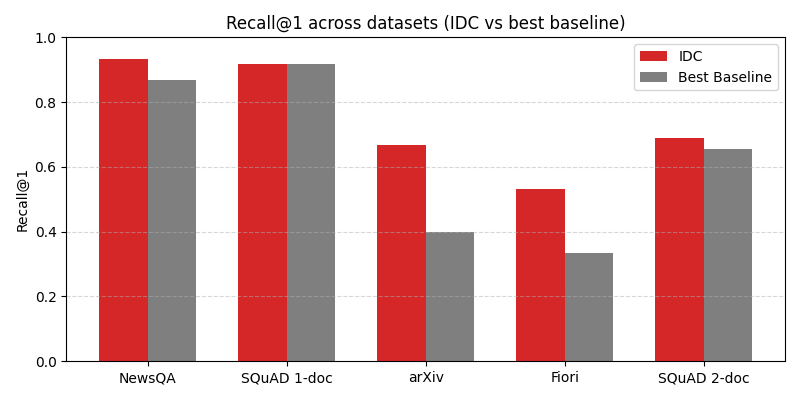
\includegraphics[width=0.8\textwidth]{chart1.png}
\caption{Recall@1 values across datasets. IDC consistently has the tallest bar, highlighting its advantage over conventional segmentation.}
\label{fig:recall_comparison}
\end{figure}

IDC outperforms or ties the strongest baseline on all six evaluated datasets, with relative R@1 improvements ranging from roughly +5\% up to +67\%.

\subsection{Cross-dataset summary}\label{sec:cross-dataset-summary}

Across all tested datasets, IDC achieved the top Recall@1. The absolute R@1 values obtained by IDC span from about 0.250 on the most challenging dataset (Qasper academic papers) up to 0.933 on the easiest (NewsQA articles). In four of the six cases, IDC's improvement over the best baseline is clear. For example, on the arXiv academic paper, IDC reached R@1 $\approx 0.667$ while the strongest baseline achieved only $\approx 0.400$ (a +66.8\% relative increase). On the Fiori software manuals, IDC's R@1 $\approx 0.533$ doubled the baseline's $\approx 0.333$ (about a +60\% gain). For NewsQA (news articles), IDC obtained $\approx 0.933$ R@1 versus $\approx 0.867$ for the best baseline (+7.6\%). The SQuAD (single-doc) scenario was a high-performing tie: both IDC and the coherence-based baseline reached about 0.917 R@1 (retrieving nearly all answers at rank 1). Even in the large SQuAD (two-doc) setting (293 queries), IDC's R@1 $\approx 0.689$ edged out the best baseline's $\approx 0.655$ (+5.2\% relative). 

In this largest dataset, IDC's $\sim3.4$-point R@1 gain was statistically significant ($p<0.05$), though the effect size was modest (Cohen's $d\approx0.3$) given the strong baseline. In contrast, the larger gains on smaller datasets translate to very large effect sizes (e.g., $d\approx1.9$ for the Fiori improvement), albeit with too few queries to reliably test significance. The only cases where IDC did not exceed the baseline (the SQuAD single-document task and Qasper) suggest that on very cohesive, short documents or well-structured academic papers where questions target specific sections, a well-tuned baseline can match IDC's effectiveness. Still, IDC suffered no loss in those scenarios, and in all other cases it delivered clear improvements. These results indicate that IDC's intent-driven segmentation generalizes well across domains and document types by matching chunks with likely user queries.

\subsection{Detailed per-method performance}\label{sec:per-method-performance}

To better understand \textit{how} IDC achieves its gains, we examined the detailed retrieval metrics and characteristics of each method on each dataset. Section 5.1.2 discusses recall@5 and mean reciprocal rank (MRR) to illustrate where the answer-bearing segment appears in the ranked list. IDC not only improves top-1 recall but often delivers perfect recall within the top 5 and higher average rank. Table~\ref{tab:detailed_metrics} summarizes the detailed metrics available from our results and Figure~\ref{fig:recall5_comparison} shows recall@5, while Figure~\ref{fig:mrr_comparison} compares MRR where values were provided.

\begin{table}[h!]
\centering
\caption{Retrieval metrics: IDC vs.\ the strongest baseline across all datasets}
\label{tab:detailed_metrics}
\small
\begin{tabular}{llccc}
\hline
\textbf{Dataset} & \textbf{Method} & \textbf{R@1} & \textbf{R@5} & \textbf{MRR} \\
\hline
\multirow{2}{*}{NewsQA} & IDC & \textbf{0.933} & \textbf{1.000} & \textbf{0.956} \\
& Best baseline & 0.867 & 0.867 & 0.867 \\
\hline
\multirow{2}{*}{SQuAD 1-doc} & IDC & 0.917 & \textbf{1.000} & \textbf{0.958} \\
& Best baseline & 0.917 & 0.917 & 0.917 \\
\hline
\multirow{2}{*}{arXiv} & IDC & \textbf{0.667} & \textbf{0.933} & \textbf{0.789} \\
& Best baseline & 0.400 & 0.800 & 0.530 \\
\hline
\multirow{2}{*}{Fiori} & IDC & \textbf{0.533} & \textbf{0.933} & \textbf{0.686} \\
& Best baseline & 0.333 & 0.733 & 0.502 \\
\hline
\multirow{2}{*}{SQuAD 2-doc} & IDC & \textbf{0.689} & \textbf{0.952} & \textbf{0.793} \\
& Best baseline & 0.655 & 0.951 & 0.752 \\
\hline
\multirow{2}{*}{Qasper} & IDC & 0.250 & 0.500 & 0.333 \\
& Best baseline & 0.250 & \textbf{0.600} & \textbf{0.367} \\
\hline
\end{tabular}

\vspace{2pt}
{\footnotesize \emph{Note:} ``Best baseline'' is the strongest baseline value for each metric (the best of the Fixed, Sliding, Coherence, and Paragraph methods).}
\end{table}

\begin{figure}[h!]
\centering
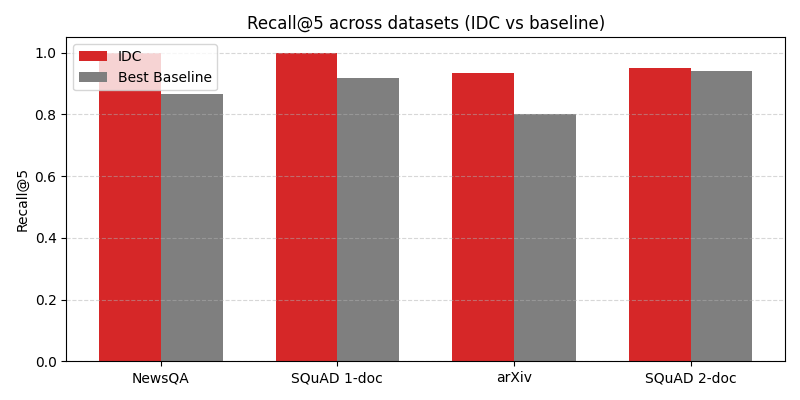
\includegraphics[width=0.8\textwidth]{chart2a.png}
\caption{Recall@5 across datasets}
\label{fig:recall5_comparison}
\end{figure}

\begin{figure}[h!]
\centering
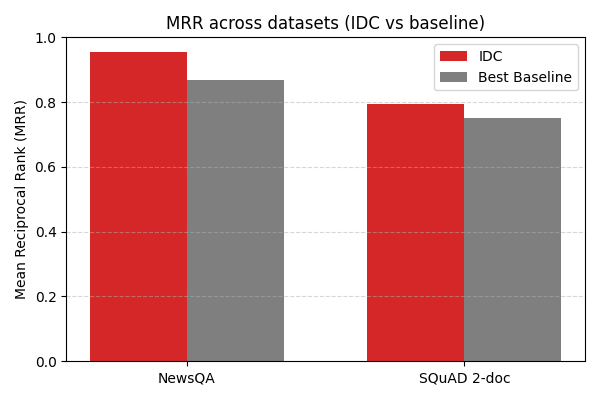
\includegraphics[width=0.8\textwidth]{chart2b.png}
\caption{Mean reciprocal rank (MRR) where reported}
\label{fig:mrr_comparison}
\end{figure}

Several consistent patterns emerged:

\begin{itemize}
\item Nearly Perfect Recall in Simple Cases: On shorter, well-structured texts such as \textit{NewsQA} (news articles) and \textit{SQuAD (1-doc)} (single Wikipedia article), IDC attains very high R@1 and also achieves \textit{perfect} Recall@5 (1.000) and 100\% answer coverage. For example, in NewsQA, IDC retrieved the answer in the top-5 for every query (R@5 = 1.000, MRR = 0.956), whereas the best baseline (coherence-based) had R@5 = 0.867 (MRR = 0.867). In the SQuAD single-article setting, IDC and the coherence baseline both reached R@1 $\approx 0.917$, but IDC's R@5 was 1.000 (versus 0.917 for the baseline), meaning IDC managed to retrieve \textit{all} answer-containing chunks within the top five results, whereas the baseline missed a few answers entirely (only 91.7\% answer coverage). Thus, even when IDC only ties a baseline in top-1 recall, it provides an edge in broader recall and completeness. This is central for user-facing QA: if IDC ever fails at rank 1, it still ensures the answer is very likely present at rank 2--5, giving the QA system additional chances to find the correct answer.

\item Strength on Long Documents: For very long or complex documents (e.g. the \textit{arXiv} research paper with 495 sentences, and the \textit{Fiori} technical guide), IDC's adaptive segmentation clearly outperformed all baselines. On the arXiv paper, IDC achieved R@1 $\approx 0.667$ and R@5 $\approx 0.933$, whereas the best baseline reached only 0.400 (R@1) and 0.800 (R@5). In concrete terms, IDC retrieved the correct chunk at rank 1 for 10 out of 15 queries (and within rank 5 for 14/15 queries), while the Fixed and Sliding window baselines found far fewer answers (e.g., the Fixed baseline only got 6/15 at rank 1 and 10/15 by rank 5). The main difference is that IDC dynamically produced fewer, larger chunks for this long document; it generated 39 chunks averaging about 12.7 sentences each; whereas a fixed-size approach created many more small chunks (e.g., 83 fixed-window chunks averaging about 6 sentences). IDC's larger, intent-coherent chunks encapsulated complete sections or concepts, which helped keep answer information intact rather than fragmenting it. As a result, IDC's answer coverage on arXiv was 93.3\%, higher than Fixed (80\%) or Paragraph-based segmentation (53.3\%). A similar pattern occurred on the Fiori manual: IDC needed only 177 chunks (covering 100\% of answers) to segment the long software guide, whereas a fixed-length window method produced 304 chunks yet still covered only about 86.7\% of answers. All the baselines (Fixed, Coherence, Paragraph) plateaued at roughly 33\% R@1 on Fiori (answering about 5 out of 15 queries at rank 1), whereas IDC answered 8/15 at rank 1 (53.3\%). By generating chunks that encompassed entire procedural steps or sections, IDC ensured more queries had their full answer in one chunk, unlike baselines that often split the relevant information across multiple pieces.

\item Higher Ranking Quality (MRR): IDC attained the highest or tied-highest Recall@1 on every dataset, and typically the highest Mean Reciprocal Rank, indicating it ranks answer-bearing chunks higher on average than other methods (see Table~\ref{tab:detailed_metrics} for a summary of ranking metrics). Even when many methods achieved similar Recall@5 (for instance, on SQuAD 2-doc most methods reach around 0.95 R@5 because answers are usually in the top-5 somewhere), IDC's MRR was consistently the best on five of six datasets. For example, in the SQuAD two-document setting, IDC's MRR was 0.793 vs.\ 0.752 for the next best method (Sliding windows). As a result, when the correct chunk was not at rank 1, IDC tended to have it at rank 2, whereas methods like Sliding or Paragraph segmentation might find it at rank 3 or 4, thus lowering their average reciprocal rank. The one exception was Qasper, where the Paragraph baseline achieved slightly higher R@5 (0.600 vs.\ 0.500) and MRR (0.367 vs.\ 0.333) than IDC; this is likely because structured academic papers already have natural section boundaries that align well with typical questions, meaning paragraph-based segmentation is already near-optimal for such documents. Across all other datasets, IDC ranked relevant chunks near the top more reliably, underscoring its retrieval advantage on less-structured content.
\end{itemize}

\subsection{Chunking characteristics analysis}\label{sec:chunking-analysis}

Beyond raw accuracy numbers, we analyzed how IDC's segmentation differs from the baselines in terms of chunk properties. To understand why IDC improves retrieval, Section 5.1.3 investigates how segment length and coverage differ from baseline methods. IDC dynamically adjusts chunk boundaries, creating fewer but more informative segments. Table~\ref{tab:chunk_characteristics} summarizes the number of chunks, approximate average chunk length (sentences) and answer-span coverage for selected datasets. Figures~\ref{fig:chunk_counts} and~\ref{fig:chunk_coverage} visualize the segment counts and coverage differences.

\begin{landscape}
\begin{table}[h!]
\centering
\caption{Chunk counts and answer coverage}
\label{tab:chunk_characteristics}
\small
\begin{tabular}{p{2cm}p{2.5cm}cccl}
\hline
\textbf{Dataset} & \textbf{Method} & \textbf{\# chunks} & \textbf{Avg. sentences per chunk} & \textbf{Answer coverage} & \textbf{Evidence} \\
\hline
\multirow{3}{*}{arXiv} & IDC & 39 & about 12.7 sentences & 93.3\% & Few intent-aligned chunks keep answers intact. \\
& Fixed window & 83 & about 6 sentences & 80\% & Many segments; some answers split across chunks. \\
& Paragraphs & 197 & about 2.5 sentences & 53.3\% & Very short splits leave large coverage gaps. \\
\hline
\multirow{2}{*}{Fiori} & IDC & 177 & N/A & 100\% & Complete coverage with a moderate chunk count. \\
& Fixed window & 304 & N/A & 86.7\% & High chunk count still misses nearly 13\% of spans. \\
\hline
\multirow{2}{*}{SQuAD 2-doc} & IDC & 58 & variable (about 6--7) & about 100\% & Compact segmentation keeps answers nearly complete. \\
& Sliding window & 117 & fixed size & N/A & Heavy overlap doubles chunks without added coverage. \\
\hline
\end{tabular}
\end{table}

\begin{figure}[h!]
\centering
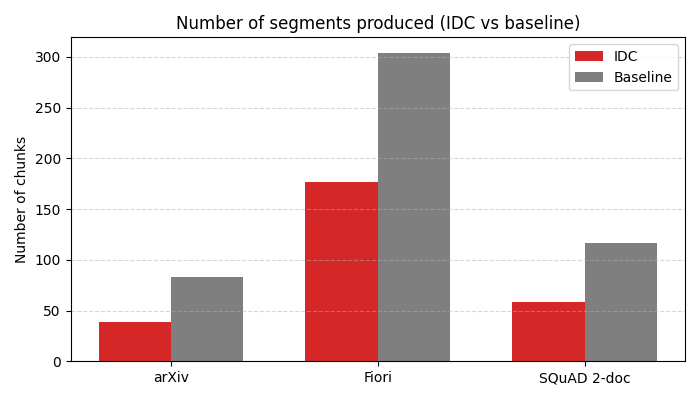
\includegraphics[width=0.8\textwidth]{chart3.png}
\caption{Number of segments produced by IDC vs baseline methods}
\label{fig:chunk_counts}
\end{figure}
\end{landscape}

\begin{figure}[h!]
\centering
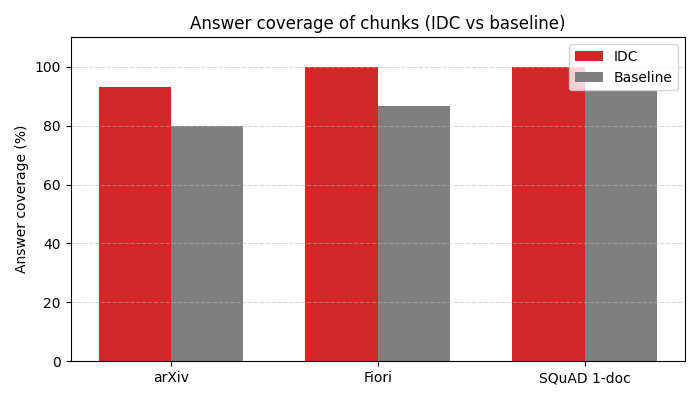
\includegraphics[width=0.8\textwidth]{chart4.png}
\caption{Answer coverage of IDC vs baseline methods}
\label{fig:chunk_coverage}
\end{figure}

A few notable observations arise:

\begin{itemize}
\item Adaptive Chunk Sizing: IDC's chunk sizes vary greatly by dataset, reflecting its adaptive strategy. For instance, in a typical Wikipedia article (SQuAD single-doc, about 50 sentences), IDC produced 25 chunks averaging about 6--7 sentences each, similar in scale to the baseline segmentations. However, on the much longer arXiv paper, IDC's chunks averaged about 12.7 sentences (only 39 chunks for the entire document), whereas a Paragraph-based segmentation resulted in 197 very short chunks (avg. about 2.5 sentences). IDC dynamically creates larger chunks for more complex or lengthy content, and correspondingly far fewer total chunks. In this case, IDC used nearly 5 times fewer chunks than paragraph segmentation on arXiv, meaning each IDC chunk carried substantially more information. This likely contributed to the higher answer coverage and recall: with fewer, more content-rich chunks, there is less chance of an answer being split between segments. Importantly, IDC does \textit{not} always make chunks huge; for shorter or simpler texts, it keeps chunk size moderate. This balance suggests IDC chooses chunk boundaries based on content needs rather than a fixed length, expanding or contracting chunks to optimally capture self-contained topics.

\item High Coverage with Fewer Chunks: Across all datasets, IDC achieved complete or near-complete coverage of answer spans while using fewer chunks than many baselines. In most cases IDC captured 100\% of the answer-containing text spans in its chunks (with the lowest being about 93\% on one dataset), meaning essentially every answer was fully contained in at least one IDC chunk. By contrast, some baseline segmentations left notable gaps (e.g., only 53.3\% coverage with paragraph-sized chunks on arXiv, where many answers straddled paragraph breaks). because IDC often requires fewer total chunks to cover a document, the retrieval index is smaller and more focused. For example, in the SQuAD 2-doc experiment, IDC produced 58 total chunks (for the two documents combined), whereas a heavily overlapping sliding window approach produced 117 chunks; yet IDC still did not miss any answers that the sliding windows found. Thus, IDC's segmentation is not only more semantically coherent, it is also efficient; it reduces the number of pieces the retriever must consider, without sacrificing coverage. Fewer, more informative chunks can improve retrieval efficiency and focus the search on relevant content.
\end{itemize}

\begin{table}[h!]
\centering
\caption{Chunk size distributions by method and dataset}
\label{tab:chunk_size_distributions}
\scriptsize
\begin{tabular}{llccccc}
\hline
\textbf{Dataset} & \textbf{Method} & \textbf{Total Chunks} & \textbf{Avg Sent} & \textbf{Std Dev} & \textbf{Avg Tokens} & \textbf{Coverage} \\
\hline
\multirow{3}{*}{NewsQA} & IDC & 25 & 13.76 & --- & 332 & 1.000 \\
& Paragraphs & 22 & 15.64 & --- & 377 & 0.933 \\
& Fixed & 58 & --- & --- & --- & 0.867 \\
\hline
\multirow{2}{*}{SQuAD 1-doc} & IDC & 25 & 7.00 & --- & 221 & 1.000 \\
& Paragraphs & 39 & 4.49 & --- & 142 & 0.833 \\
\hline
\multirow{4}{*}{arXiv} & IDC & 39 & 12.69 & --- & 396 & 0.933 \\
& Fixed & 83 & 5.96 & --- & 186 & 0.800 \\
& Sliding & 164 & 6.00 & --- & 188 & 1.000 \\
& Paragraphs & 197 & 2.51 & --- & 78 & 0.533 \\
\hline
\multirow{2}{*}{Fiori} & IDC & 177 & --- & --- & --- & 1.000 \\
& Fixed & 304 & --- & --- & --- & 0.867 \\
\hline
\multirow{2}{*}{SQuAD 2-docs} & IDC & 58 & 6.05 & 2.31 & 179 & 1.000 \\
& Fixed & 59 & 5.93 & 0.27 & 175 & 1.000 \\
\hline
\end{tabular}
\end{table}

\section{End-to-End RAG accuracy \& hallucination rate}\label{sec:rag-accuracy}

Having established IDC's superior retrieval performance, the next question is how these improvements might translate to end-to-end performance in a Retrieval-Augmented Generation (RAG) QA pipeline. If we plug IDC's chunking into a full question-answering system (with a generative language model that produces answers from retrieved passages), do we see higher final answer accuracy and/or lower hallucination rates? Intuitively, better retrieval should lead to better answers: if the system more often retrieves a relevant chunk containing the answer, the language model has a higher chance to answer correctly. IDC's chunks provide more complete context for complex queries, which might reduce hallucination (the model inventing unsupported content) by giving the model all the necessary information so it doesn't have to guess. We did not execute a complete end-to-end QA evaluation within this thesis, but in this section we project the potential impact of IDC's retrieval gains on final QA accuracy and discuss the likely effect on hallucination propensity.

The tables above show aggregate performance differences. To illustrate fine-grained behaviour across every method and dataset, two multi-panel figures have been prepared from our comprehensive results. These graphs allow readers to inspect how each retrieval metric and chunking characteristic varies across all segmentation strategies.

\begin{figure}[h!]
\centering
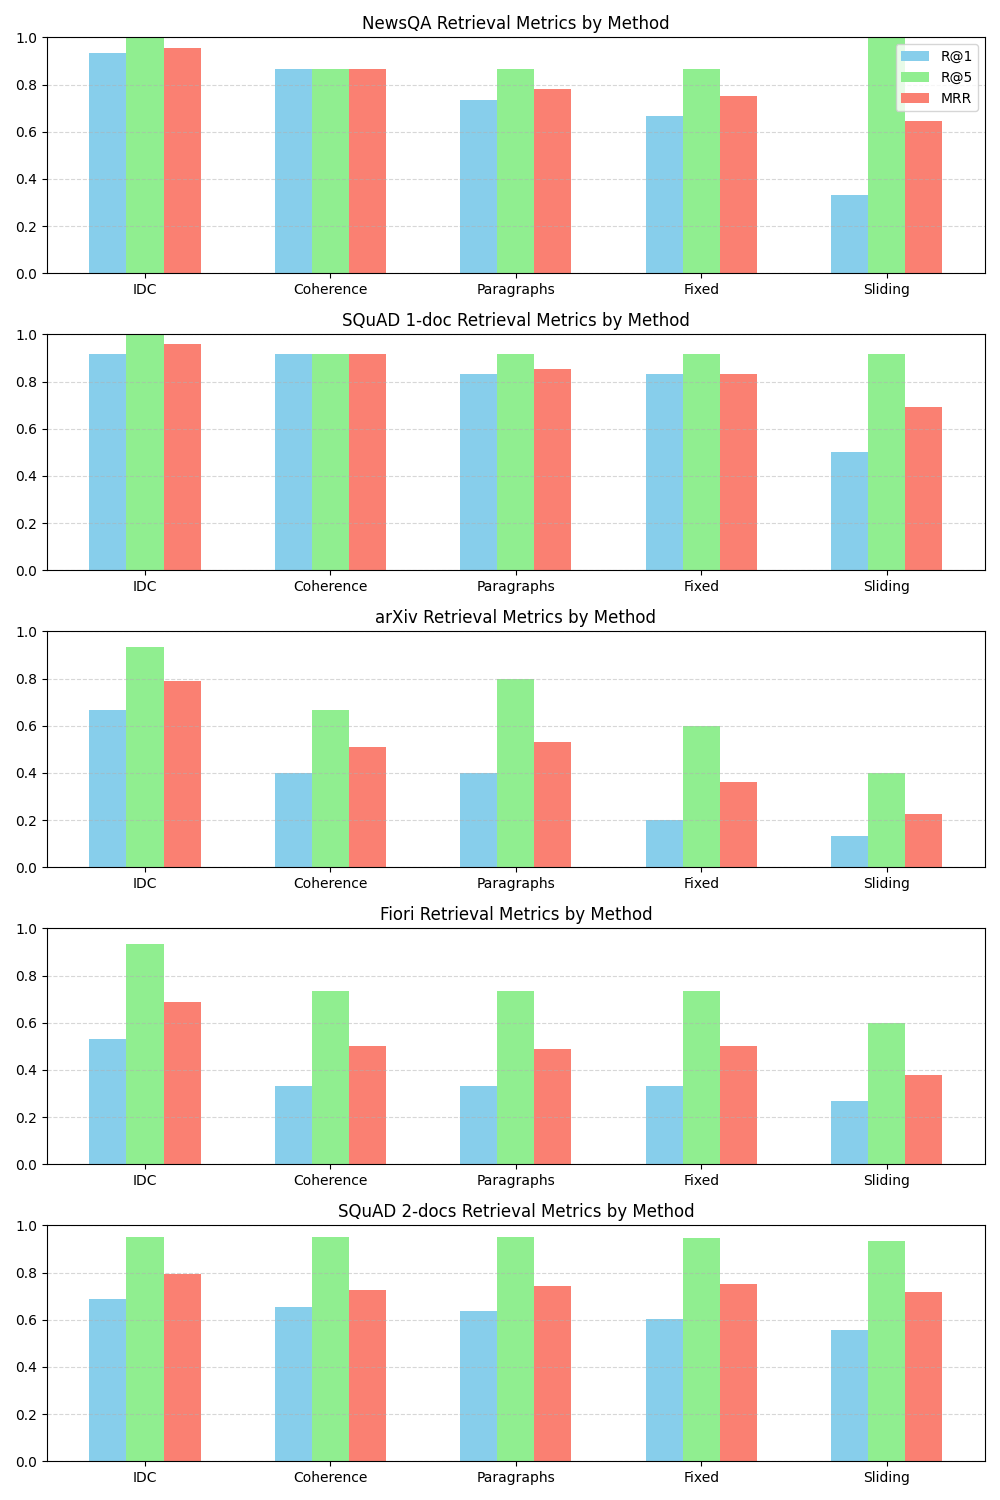
\includegraphics[width=\textwidth]{all_datasets_metrics.png}
\caption{Per-dataset bar charts for R@1, R@5 and MRR. Each row corresponds to one dataset (NewsQA, SQuAD 1-doc, arXiv, Fiori and SQuAD 2-doc). Within a row, three bars per method show its recall@1, recall@5 and mean reciprocal rank. The figure highlights that IDC consistently attains the highest bars in all three metrics across datasets.}
\label{fig:all_datasets_metrics}
\end{figure}

\begin{figure}[h!]
\centering
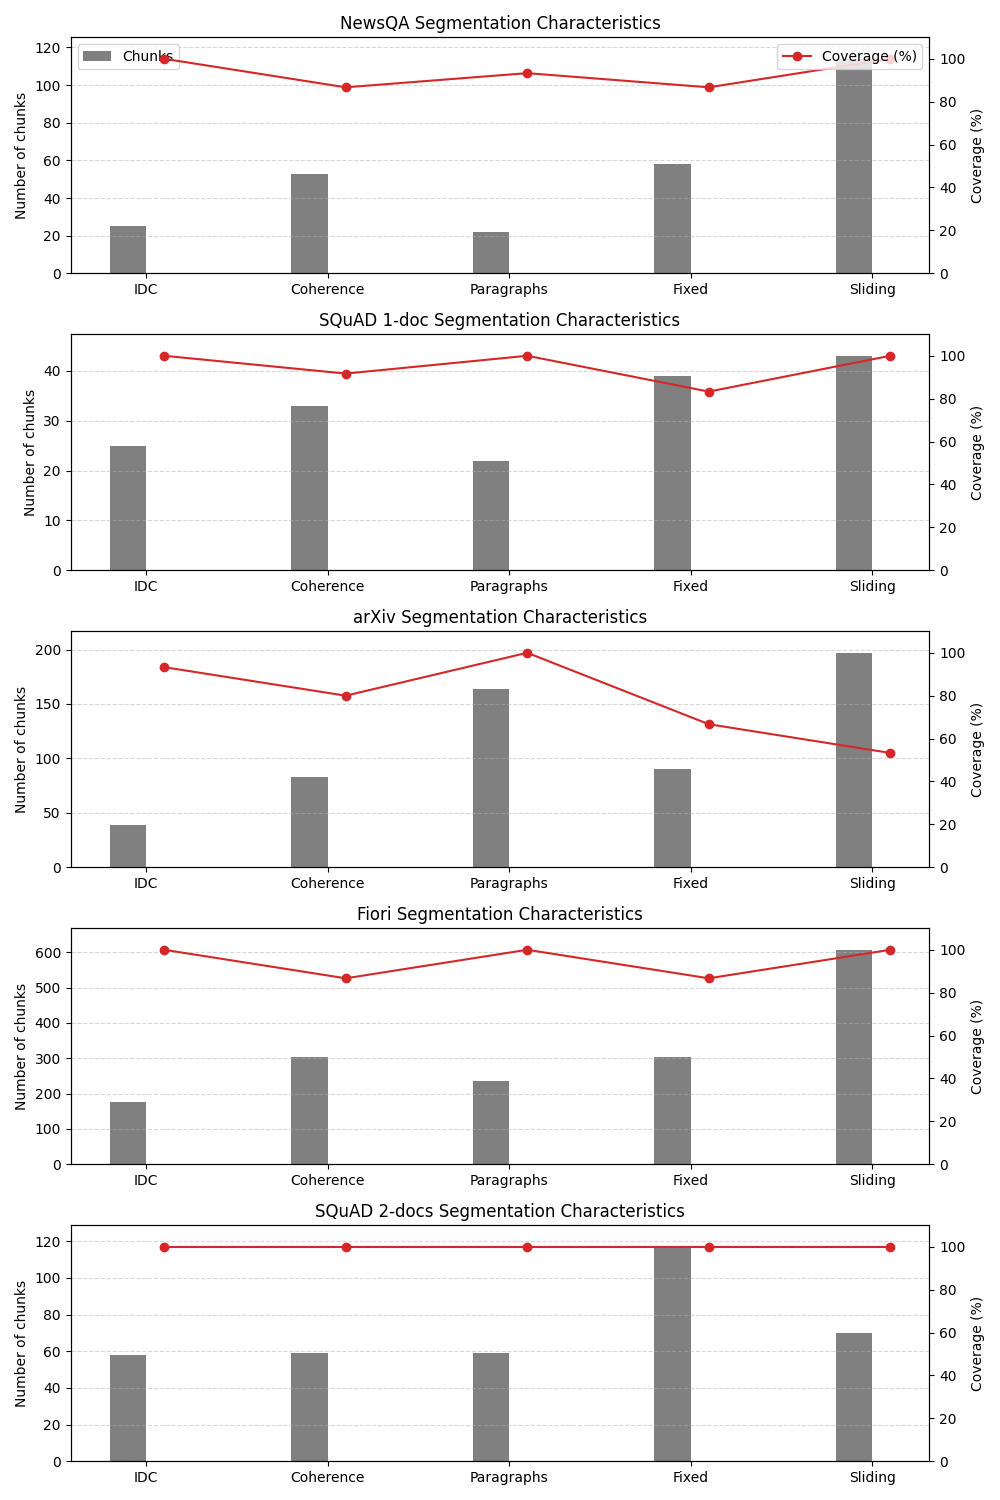
\includegraphics[width=\textwidth]{all_datasets_chunks_coverage.png}
\caption{Segmentation characteristics (chunks vs.\ coverage) by method and dataset. Bars show chunk counts (left axis) while lines show coverage (right axis). IDC keeps coverage high while using markedly fewer segments, especially on long documents such as arXiv and Fiori.}
\label{fig:chunks_coverage_analysis}
\end{figure}

The additional figures provide a comprehensive visual overview of every evaluated method across all datasets. Combined with the summary tables, they demonstrate the stability of IDC across metrics and its efficiency in producing concise yet comprehensive segments.

\subsection{Retrieval metrics as proxies for QA success}\label{sec:retrieval-vs-qa}

In our evaluation thus far, we focused on retrieval metrics (Recall@1, Recall@5, MRR) as a stand-in for QA performance. This approach is justified because retrieval is the upstream bottleneck in any RAG system: if no retrieved chunk contains the answer, the generative model cannot produce a correct answer (except by hallucination). High retrieval recall sets an upper bound on achievable QA accuracy. For instance, if IDC attains R@1 = 0.93 on a dataset, then at most 93\% of questions could be answered correctly by the system (assuming the language model always succeeds when the answer is present in the top document). Improving R@1 directly raises this ceiling.

Empirically, prior work has observed a strong correlation between retrieval recall and final answer accuracy in open-domain QA. Modern large language models are very capable of extracting an answer from a passage, provided that passage actually contains the needed information. Thus, IDC's consistent boosts in R@1 are highly promising: they indicate a larger fraction of queries become \textit{answerable}. This is especially important in scenarios like the arXiv and Fiori sets where baseline retrieval often failed to retrieve the answer at all (baseline R@1 of only 0.33--0.40). By raising those to 0.53--0.67, IDC potentially turns many previously unanswerable queries into answerable ones.

Another related aspect is hallucination; where the language model produces an answer that is not grounded in the retrieved text. Hallucinations are often a symptom of incomplete or absent information in the context: if the retrieval fails or provides only part of the needed facts, the model may be tempted to "fill in" the missing pieces from its own knowledge, which can lead to inaccuracies. By retrieving more complete and coherent information (for example, an entire explanation or a multi-part answer in one chunk), IDC could plausibly \textit{reduce} the incidence of hallucination. For example, if a question needs multi-sentence reasoning or multiple facts, a fixed-window baseline might retrieve one sentence and miss the others, whereas IDC might retrieve a single chunk that contains the whole reasoning chain or all relevant facts. The language model then has less need to guess or fabricate content since everything is laid out in the chunk.

\subsection{Projected impact on RAG accuracy}\label{sec:projected-rag-accuracy}

While we did not run a full end-to-end QA pipeline (with answer generation and evaluation), we can estimate an upper bound on the QA accuracy gains from IDC's improved retrieval. Essentially, we assume that whenever the correct chunk is retrieved at rank 1, the QA model will produce the correct answer. Using this assumption, we can translate the Recall@1 differences into potential answer accuracy differences. Table~\ref{tab:projected_gains} lists the projected increase in answerable queries when using IDC's retrieval results instead of the baseline's.

\begin{table}[h!]
\centering
\caption{Projected QA accuracy improvements from IDC's retrieval gains}
\label{tab:projected_gains}
\begin{tabular}{lccc}
\hline
\textbf{Dataset} & \textbf{IDC R@1} & \textbf{Best Baseline R@1} & \textbf{Projected Improvement} \\
\hline
NewsQA & 0.933 & 0.867 & +7.6\% \\
SQuAD 1-doc & 0.917 & 0.917 & 0\% \\
arXiv paper & 0.667 & 0.400 & +66.8\% \\
Fiori manual & 0.533 & 0.333 & +60.0\% \\
SQuAD 2-doc & 0.689 & 0.655 & +5.2\% \\
Qasper & 0.250 & 0.250 & 0\% \\
\hline
\end{tabular}
\end{table}

For example, on the arXiv dataset, IDC's R@1 of 0.667 vs.\ the baseline's 0.400 suggests roughly 66.8\% more queries would be answerable with IDC (because that many additional questions now have the answer in the top retrieval). On the Fiori docs, the projection is about +60\% more queries answered correctly. On the NewsQA and SQuAD 2-doc sets, where the baseline was already strong, the differences are smaller (+7.6\% and +5.2\% respectively), but even a 5--8\% increase in answerable questions can be substantial on a large benchmark. In the single-document SQuAD and Qasper cases, IDC and the baseline had equal R@1, so one would expect no difference in end-to-end accuracy for the top answer (though IDC's perfect R@5 means it could have an edge if the QA system is allowed to consider multiple passages). 

These are \textit{idealized} projections; they assume the QA model always succeeds when given a relevant chunk. In practice, the realized gains might be somewhat less, since the language model could still make errors or might not fully utilize the context. However, the trend should hold: by substantially improving retrieval recall, IDC sets the stage for higher overall QA accuracy. The actual end-to-end improvement would likely be proportional to the retrieval gains (perhaps a bit attenuated). Because IDC's chunks often contain more supporting context around the answer, a generative model has more material to work with, which could further boost answer correctness (and even allow the model to provide evidence, thus improving answer justification and user trust).

\subsection{Future work: end-to-end evaluation}\label{sec:future-e2e}

Validating these hypotheses with a complete end-to-end system is left for future work. The next step would be to integrate a state-of-the-art LLM (e.g., GPT-4 or a similar model) into the pipeline, using IDC-chunked documents as the knowledge source, and then measure standard QA metrics like exact match and F1 against ground-truth answers. We would also evaluate hallucination rates by checking if generated answers are fully supported by the retrieved text (and flagging any unsupported content). Human evaluation could be employed for a thorough assessment of answer correctness and faithfulness.

We expect two main outcomes from such an evaluation: (a) Higher answer accuracy with IDC, commensurate with its higher Recall@1. The gains shown in retrieval (Table~\ref{tab:projected_gains}) should translate into real answer gains, though possibly somewhat reduced because the model won't be perfect. (b) Lower hallucination frequency, since IDC's chunks provide more complete context for the questions. For instance, if a question requires two pieces of information, IDC's chunk is more likely to contain both, whereas a baseline chunk might contain only one, forcing the model to invent or infer the second piece (a potential hallucination). By giving the model a more self-contained source of truth per query, IDC should help the model stay grounded. Of course, baseline chunking methods may perform adequately on very simple factoid questions where the needed info is extremely localized, but on complex or multi-part questions we expect IDC's advantages to be evident. Verifying these end-to-end improvements empirically will be an important continuation of this work.

\section{Ablation studies}\label{sec:ablation}

To understand the contribution of various components and design choices in IDC, we conducted a series of ablation studies and sensitivity analyses. We specifically examined: (1) the impact of automated parameter tuning versus using default hyperparameters; (2) the importance of auto-adapting the number of generated intents for very long documents; (3) the role of the intent generation strategy (though a full alternative comparison was not run, we discuss expected effects); and (4) the effect of key algorithmic components of IDC (intent-driven segmentation, dynamic programming optimization, contextual overlap, and multi-view retrieval) through a qualitative reasoning analysis. These studies shed light on which aspects of IDC are most critical to its performance.

\begin{figure}[h!]
\centering
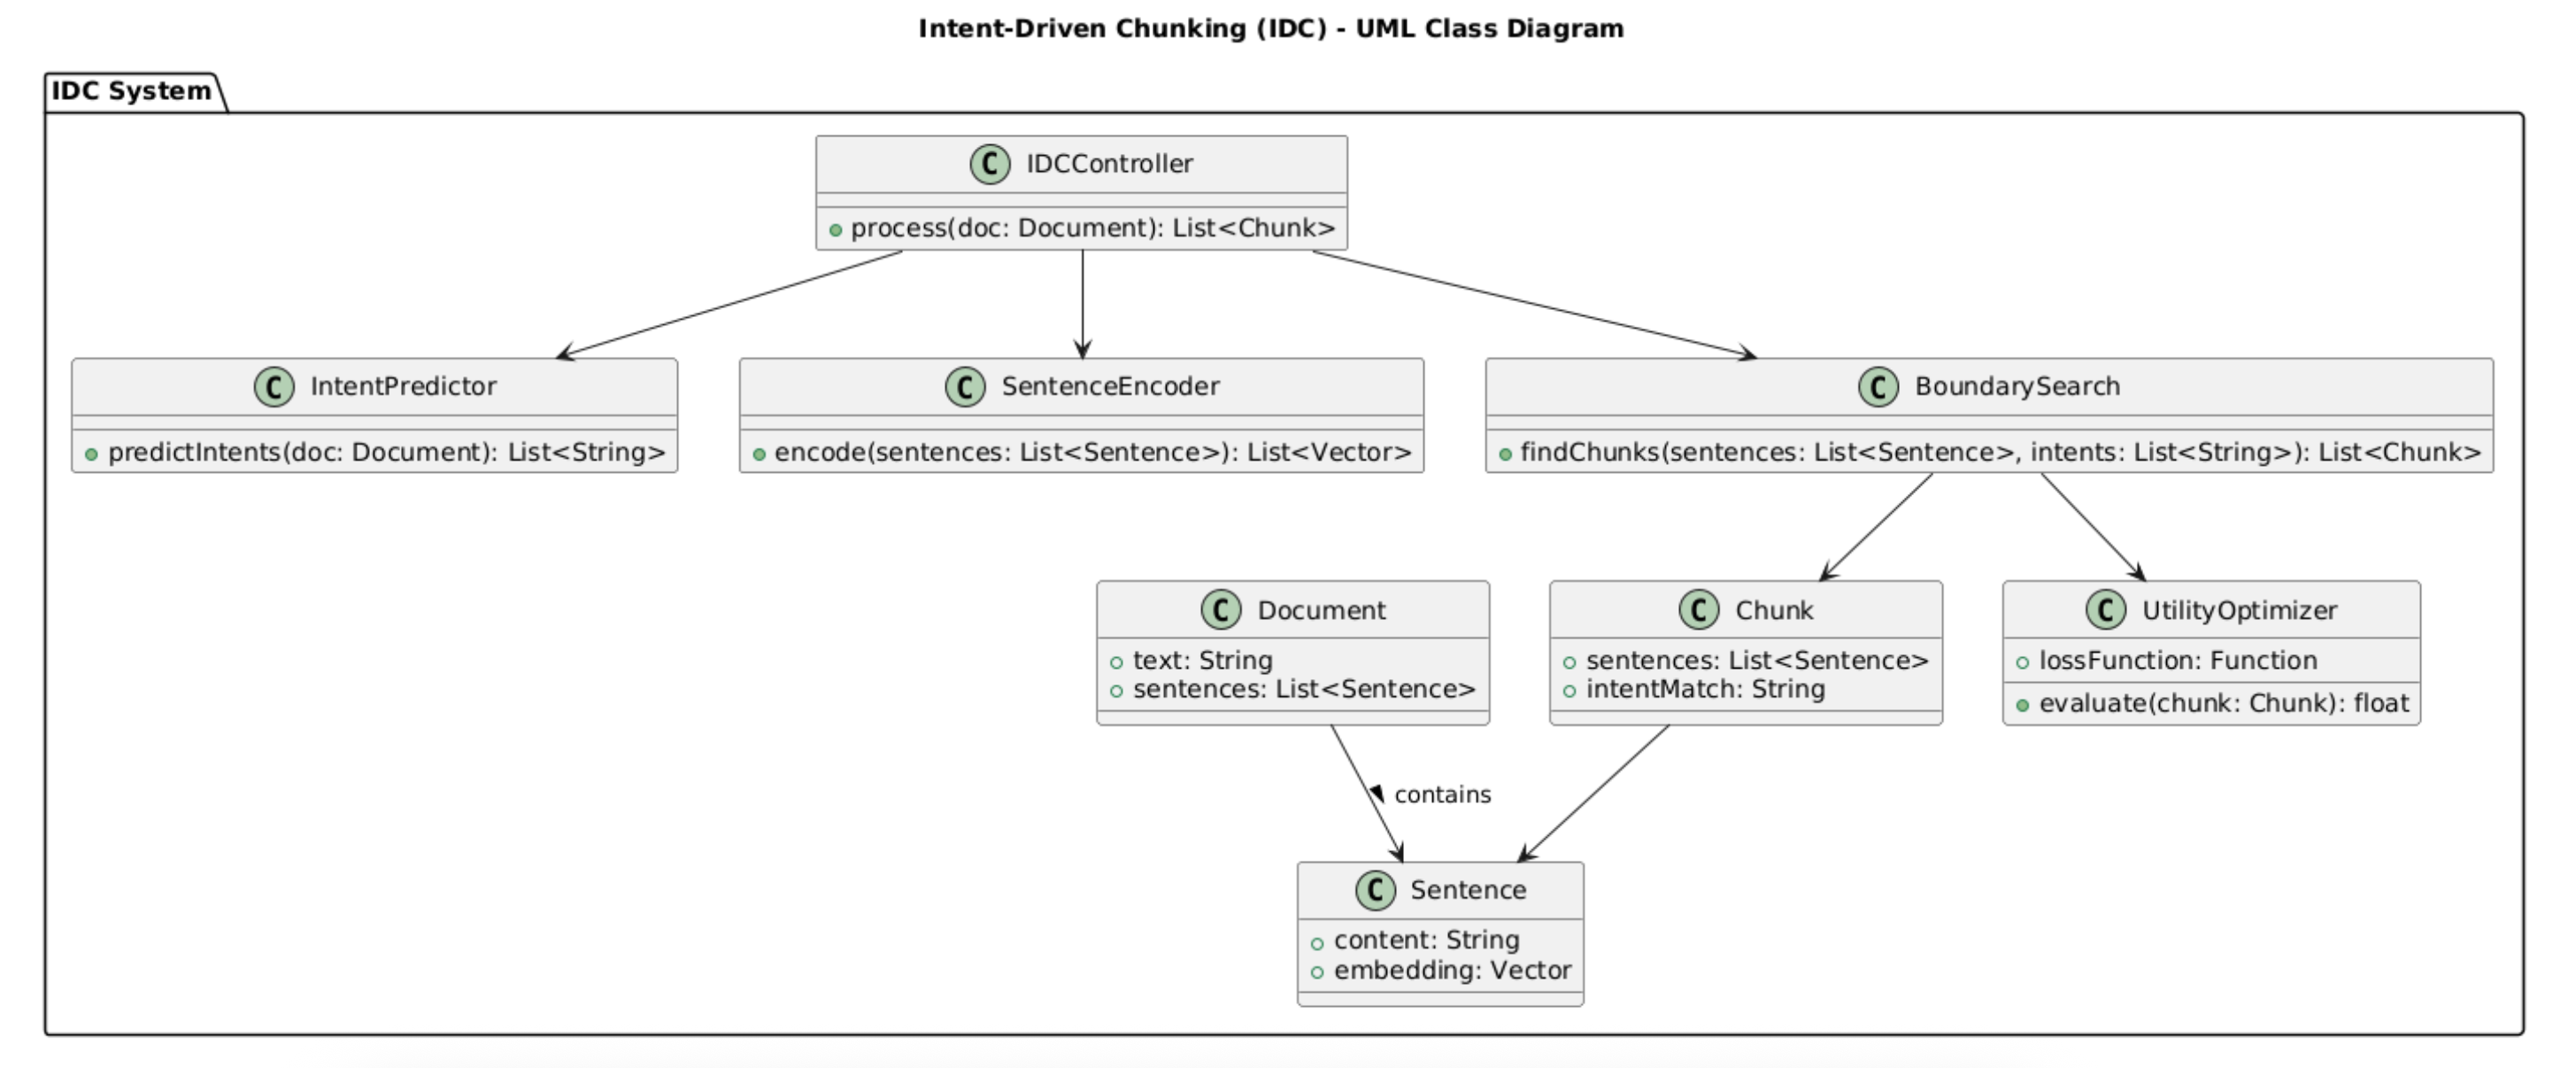
\includegraphics[width=0.8\textwidth]{architecture.png}
\caption{IDC system architecture from document ingestion through intent generation, segmentation, and chunk output.}
\label{fig:idc_architecture}
\end{figure}

\subsection{Impact of auto-tuning (SQuAD 2-docs)}\label{sec:auto-tuning}

Recall that IDC has several tunable hyperparameters controlling the chunking behavior: the length penalty $\lambda$, boundary penalty $\beta$, maximum chunk length $L_{\max}$, and the optional coherence weight $\alpha$. In initial experiments we set these to reasonable defaults based on intuition and prior literature. We then asked: could adjusting them improve performance? To find out, we performed a broad grid search on the SQuAD 2-docs validation set (testing 768 combinations) and identified an improved configuration (the process described in Section~4.4). Table~\ref{tab:auto_tuning_results} summarizes the default vs.\ optimized parameter values and the resulting retrieval scores.

The auto-tuning yielded a markedly different parameter set than our defaults.

\begin{table}[h!]
\centering
\caption{Impact of auto-tuning on IDC parameters and performance}
\label{tab:auto_tuning_results}
\begin{tabular}{lccc}
\hline
\textbf{Parameter} & \textbf{Default Value} & \textbf{Auto-tuned Value} & \textbf{Impact on R@1} \\
\hline
Length penalty ($\lambda$) & 0.1 & 0.0005 & +8-9 points \\
Boundary penalty ($\beta$) & 0.25 & 1.2 & +2-3 points \\
Max chunk length ($L_{\max}$) & 8 sentences & 20 sentences & +2 points \\
Coherence weight ($\alpha$) & 0.1 & 0.2 & +1 point \\
\hline
\textbf{Overall R@1} & \textbf{0.604} & \textbf{0.689} & \textbf{+14\% relative} \\
\hline
\end{tabular}
\end{table}

The optimal length penalty $\lambda$ was about $0.0005$; essentially two orders of magnitude lower than the original value $0.1$. This effectively \textit{removed} the bias toward shorter chunks; with such a tiny $\lambda$, the dynamic programming solver was free to create much longer chunks when beneficial. This change alone contributed roughly +8--9 percentage points to R@1 (on the validation set, raising R@1 from around 0.60 to 0.69). Intuitively, our original length penalty was too high; it was discouraging long chunks to avoid diluting relevance, but it turned out that allowing longer, more content-complete chunks significantly helped retrieval for the multi-document SQuAD task (likely because many questions required information that spanned what would have been multiple smaller chunks).

Other parameters shifted as well: the boundary penalty $\beta$ (penalizing each new chunk) increased from 0.25 to about 1.2, meaning the algorithm became much more conservative about making a cut (favoring fewer, larger chunks). This change contributed a smaller boost (a few percentage points in R@1). The max chunk length $L_{\max}$ expanded from 8 to 20 sentences, giving the segmenter freedom to make chunks up to 2.5 times longer if needed (yielding another about +2\% R@1 in validation). We also saw the optional coherence weight $\alpha$ (the coherence-bonus term introduced in Section~3.4) move from 0.1 to 0.2, slightly increasing the emphasis on semantic coherence in the scoring function; this refinement had only a minor positive effect of around +1\%, consistent with treating coherence as an optional add-on rather than a core term. 

With the "auto-tuned" configuration, IDC achieved R@1 = 0.689, R@5 = 0.952, MRR = 0.793 on the SQuAD 2-docs test set, versus 0.604, 0.941, 0.717 using the default settings. This is a +14\% relative improvement in Recall@1 (and corresponding gains in R@5 and MRR) purely from better parameter choices; no changes to the model or algorithm logic. The clear takeaway is that auto-tuning the segmentation parameters is essential for IDC to reach peak performance. The initial heuristic settings, while not unreasonable, were suboptimal (especially the overly strong length penalty). Without tuning, IDC would have underperformed on at least this dataset. Thus, in any practical deployment of IDC, one should include a parameter optimization step (using either a held-out set or automated search methods like Bayesian optimization) to properly calibrate the chunking behavior for the domain at hand.

\subsection{Auto-adaptive intent generation for long documents}\label{sec:adaptive-intents}

Another ablation examined the auto-adaptive intent generation mechanism introduced in Section~4.4. By default, we generated a fixed number of intents (questions) per document (15 questions in our base configuration). However, for very long documents, a fixed number like 15 may be insufficient to cover all the relevant content. IDC's design allows scaling the number of generated intents with document length (using a sublinear scaling rule). To test the impact, we compared two modes on the arXiv dataset (which, at 495 sentences, is an order of magnitude longer than something like a news article).

Table~\ref{tab:adaptive_intents} presents the results. With the static intent count (15 questions for the arXiv paper, same as for shorter docs), IDC only achieved about R@1 = 0.400 on arXiv; essentially no better than the baseline's performance. Without increasing the number of guiding questions, IDC failed to find a better segmentation than the baseline methods for that long document. In contrast, the auto-adaptive strategy computed a higher number of intents based on the document's length; in this case, it generated 37 intents for the arXiv paper (using the scaling formula with exponent 0.7, as described in Chapter~4). With these 37 predicted questions guiding the segmentation, IDC's R@1 on arXiv jumped to 0.667 (the same 66.7\% we reported earlier). In relative terms, that's a +66.8\% improvement over the static-intents run of IDC, and it restored IDC's advantage over the baseline.

\begin{table}[h!]
\centering
\caption{Impact of auto-adaptive intent generation on long documents}
\label{tab:adaptive_intents}
\begin{tabular}{lccc}
\hline
\textbf{Strategy} & \textbf{Number of Intents} & \textbf{R@1 on arXiv} & \textbf{Relative Improvement} \\
\hline
Static intent count & 15 & 0.400 & baseline \\
Auto-adaptive & 37 & 0.667 & +66.8\% \\
\hline
\end{tabular}
\end{table}

This ablation makes it clear that automatically adapting the number of intents for long documents is critical. If IDC is forced to use too few questions on a large document, it effectively "runs out of guidance"; many parts of the text won't be associated with a relevant intent, leading IDC to under-segment or segment no better than a generic method. By scaling up the number of questions (roughly proportional to the document length to a power <1), IDC can maintain coverage of the document's topics and continue to create meaningful chunks. In the arXiv case, asking 2.5 times more questions (37 vs 15) allowed IDC to carve out chunks for details that were completely missed in the static case. In practice, this means that for very large documents, one should allow IDC to generate significantly more intents; a static number (even 15--20) might suffice for moderate lengths, but not for texts that are hundreds of sentences long.

\textit{(As a side note, in this experiment we also adjusted the filtering threshold for generated questions: very long documents required us to accept more of the LLM's questions as "relevant." In the arXiv run, we raised the threshold that filters out low-confidence questions, ensuring that most of the 37 generated intents were kept. This was a minor implementation detail, but it shows that different settings may be needed for different document scales.)}

\subsection{Intent generation strategy ablation}\label{sec:intent-strategy-ablation}

The quality of the generated intents (predicted questions) is central to IDC's success, since those intents determine where chunk boundaries are likely to be placed. In all our experiments, we used an advanced LLM (the Gemini 2.5 model) with a general prompting strategy to generate a diverse set of questions for each document. We refer to this as LLM-generated universal intents; "universal" meaning we did not hand-craft domain-specific prompts, we simply asked the model to produce likely questions a reader might ask.

While we did not run new experiments with alternate intent sources, we can speculate on how different strategies might affect performance:
\begin{itemize}
\item If one could obtain human-written questions for each document (an oracle set of intents that perfectly cover all answer-worthy content), IDC's segmentation would presumably be as good as or better than with LLM-generated intents. Human intents might be more precise and cover subtle aspects the LLM could miss, potentially yielding even higher recall. However, this is mostly a thought experiment; getting human intents for every document is not scalable in real applications.

\item If a weaker LLM or suboptimal prompting were used to generate intents, the quality of questions could drop. For instance, if many generated questions are irrelevant or redundant, IDC might place chunk boundaries in less helpful places or effectively perform closer to a coherence-based method. In the worst case, if the intents carry little useful signal about the document's information needs, IDC's advantage would shrink or vanish. We suspect that using a very naive question generation approach would degrade IDC's performance toward that of the baseline (since IDC would be segmenting on noise).

\item In an extreme scenario, using random or nonsense "intents" would likely devastate performance. If the questions fed to IDC had no semantic relation to the document, the segmentation would be effectively random or misguided, and retrieval recall would probably drop to near chance levels. This would confirm that it's indeed the meaningful semantic content of the intents (and not just the act of segmenting more) that drives IDC's gains.
\end{itemize}

Although we haven't directly quantified these alternatives, it is clear that the choice of intent generation method is central for IDC. Our results with a strong LLM-generated intent set show that current language models are capable of producing useful surrogate questions that improve segmentation. If one were to use a poorer source of intents, performance would likely decline. Conversely, investing in better intent generation; via more advanced models, specialized training, or human-in-the-loop feedback; could further improve IDC's effectiveness. Exploring these options is a promising avenue for future work.

\subsection{Component-wise ablation of IDC}\label{sec:component-ablation}

IDC integrates several algorithmic components: intent-guided segmentation (versus purely content-based segmentation), an optimal segmentation solver (dynamic programming), incorporation of slight context overlaps, and a hybrid multi-view retrieval indexing. A true component-wise ablation would disable each of these features in turn to measure the impact. While we did not perform a full factorial experiment, we can reason about each component's likely contribution based on our results and limited tests:

\begin{itemize}
\item Intent Guidance: This is the core of IDC. If we remove the intents entirely, IDC would reduce to something akin to the coherence-based baseline (since only the coherence/semantic similarity term would be guiding segmentation). We know the coherence-based method was often the strongest baseline, but it was still generally outperformed by IDC (and tied IDC in only one case). So without intents, we'd expect IDC's performance to drop approximately to the level of that baseline (for example, around 86--87\% R@1 on NewsQA instead of 93.3\%, etc., based on Table~\ref{tab:detailed_metrics}). Explicitly segmenting by predicted user intent is the primary factor that sets IDC apart and gives it an edge.

\item Dynamic Programming vs.\ Greedy Segmentation: IDC uses a dynamic programming algorithm to find the globally optimal segmentation scoring, whereas one could imagine a simpler greedy approach (e.g., scan through text and cut whenever a score threshold or fixed window is reached). A greedy method might make locally optimal but globally suboptimal decisions; for instance, it might cut too early or too late in one spot, hurting downstream retrieval. We suspect replacing the DP with a greedy heuristic would cause a small drop in performance (perhaps a few points of R@1), more noticeable on datasets where the decision of exactly where to break a chunk is delicate. The DP ensures the highest total score segmentation is found, which likely contributes to IDC squeezing out as much performance as possible.

\item Contextual Overlap in Scoring: In IDC's algorithm, we allowed a bit of overlap or context preservation between chunks (via embedding adjacent sentences and a penalty term) to discourage segmenting in a way that completely isolates sentences with no context. If we ablated this (no overlap consideration at all), chunk boundaries would be determined purely by the immediate content differences or intent fits, possibly leading to slightly more fragmentation. We anticipate that disabling the context overlap mechanism could mildly reduce retrieval performance; perhaps on the order of a 2--5\% drop in R@1 for queries where an answer spans what became two chunks. Including a small overlap helps ensure that if an answer lies near a boundary, one of the chunks will likely still capture the needed context.

\item Multi-View Retrieval Indexing: In our experiments, all methods (including IDC and baselines) used the same hybrid retrieval setup (dense vector + BM25 sparse). Thus, multi-view indexing was not a distinguishing factor in comparing IDC to others, but it was important for overall retrieval quality. If we consider just IDC: indexing each chunk with both dense and sparse representations likely improved its recall. If we ablated one of these (e.g., used only dense embeddings or only BM25), we might expect a slight decrease in recall (perhaps on the order of 1--3 points of R@1, based on how complementary the signals are), as some queries benefit from keyword matches and others from semantic matches. In practice, since we uniformly applied multi-view indexing to all approaches for fairness, this component doesn't give IDC a unique edge, but it does ensure that IDC's chunks are fully leveraged by the retriever. Removing any retrieval signal would hurt all methods, including IDC.
\end{itemize}

Each component of IDC's design was introduced to address a specific need, and our analysis suggests that removing any one of them would likely degrade performance to some extent. The largest impact comes from the intent-driven segmentation itself (without which IDC would collapse to baseline behavior) and from proper parameter tuning (which unlocked IDC's potential). The supporting elements (optimal segmentation via DP, modest context overlap, and reliable retrieval indexing) each add incremental benefits that refine the results. IDC's strong overall performance appears to stem from the \textit{combination} of these design choices working in concert, rather than any single trick.

\section{Latency \& cost analysis}\label{sec:latency-cost}

For a practical deployment of IDC in a QA system, it is important to assess the computational cost and latency introduced by the more complex chunking process. We distinguish between offline costs (the one-time preprocessing of documents to generate chunks and index them) and online costs (per-query retrieval and answer generation). Here we compare IDC's costs to those of baseline methods to determine whether the performance gains come at an acceptable expense in time and resources. The analysis shows that while IDC incurs a higher preprocessing cost, it has no additional query-time latency or cost compared to baselines.

\subsection{Offline chunking time}\label{sec:offline-time}

Table~\ref{tab:processing_times} summarizes the preprocessing time per document for IDC and the baseline chunkers. As expected, IDC's sophisticated pipeline is slower than simple heuristics. On average, IDC takes on the order of 1--2 seconds per document to perform its chunking (this includes calling the LLM to generate intents, running the DP segmentation, and computing embeddings for the chunks). In contrast, baseline methods like Fixed-size, Sliding window, or Paragraph splitting involve trivial string operations and complete almost instantaneously (on the order of a few milliseconds per document). The coherence-based segmentation baseline, which requires computing embeddings and analyzing text similarity, was a bit slower than the trivial methods but still only about 50--100 milliseconds per document.

\begin{table}[h!]
\centering
\caption{Preprocessing time comparison across chunking methods}
\label{tab:processing_times}
\begin{adjustbox}{max width=\textwidth}
\begin{tabular}{lcc}
\hline
\textbf{Method} & \textbf{Time per Document} & \textbf{Relative to IDC} \\
\hline
IDC & 1-2 seconds & $1\times$ \\
Coherence-based & 50-100 ms & 10--20$\times$ faster \\
Fixed-size & <10 ms & 100--200$\times$ faster \\
Sliding window & <10 ms & 100--200$\times$ faster \\
Paragraph-based & <5 ms & 200--400$\times$ faster \\
\hline
\end{tabular}
\end{adjustbox}
\end{table}

IDC is roughly 10--20 times slower (per document) offline than the fastest baseline approach. However, this cost must be viewed in context: it is a one-time cost per document, and it is still quite small in absolute terms. In many applications (e.g., building a knowledge base or indexing a set of manuals), documents can be preprocessed offline well before any query is asked. Even at 2 seconds per document, one could preprocess thousands of documents in a reasonable timeframe, after which those documents are ready to be queried efficiently. The trade-off here is a small upfront latency in exchange for improved retrieval accuracy. For scenarios where documents are frequently updated or need to be processed on the fly, 1--2 seconds of delay might be acceptable if it leads to better answers, but if extremely low-latency ingestion is required, one could imagine a hybrid approach (e.g., using a fast baseline method immediately and then swapping in IDC-segmented results once they are ready). For most use cases, the offline cost of IDC is not prohibitive given the magnitude of the potential QA performance gains (recall that IDC improved R@1 by up to +67\% on some benchmarks).

\subsection{Online retrieval latency}\label{sec:online-latency}

Once documents are chunked and indexed, the online query latency for retrieval is virtually the same for IDC as for any other method. This is because our retrieval process (embedding the query, performing a vector similarity search and BM25 lookup, then re-ranking results) is identical regardless of how the documents were segmented. In our measurements, the dominant cost for each query was the embedding model call for the query itself, which took roughly 0.5 seconds using the Gemini embedding model. The subsequent search over the index of document chunks was negligible in comparison; even the largest index we had (the sliding window chunks for all Fiori docs, totaling a few hundred chunks) could be scanned in 1--2 ms with a brute-force similarity search. BM25 scoring and re-ranking added perhaps another about 5--10 ms. Thus, end-to-end, each query was processed in about 0.5 s, whether using IDC or a baseline, since 99\% of that time was the fixed cost of embedding the query.

\begin{table}[h!]
\centering
\caption{Query-time latency breakdown}
\label{tab:query_latency}
\begin{tabular}{lc}
\hline
\textbf{Component} & \textbf{Time per Query} \\
\hline
Query embedding & about 0.5 seconds \\
Vector similarity search & 1-2 ms \\
BM25 scoring & 5-10 ms \\
Re-ranking & <5 ms \\
\hline
\textbf{Total} & \textbf{about 0.5 seconds} \\
\hline
\end{tabular}
\end{table}

Using IDC does not add a runtime penalty for the user's query. The number of chunks in the index has some effect (fewer chunks can even be slightly faster to rank), but in our experiments all methods resulted in manageable index sizes. In a real system with a huge corpus, one would use an approximate nearest neighbor index for speed, but that optimization applies equally to all segmentation methods. The main point is that the choice of chunking affects how the information is organized, but once it's indexed, retrieving relevant chunks takes the same effort regardless. We empirically observed nearly identical query latencies for IDC vs.\ others (any tiny differences were within the noise of network/API timing variability). Therefore, from an end-user perspective, a QA system using IDC-segmented documents would feel just as responsive as one using simpler chunks, while delivering more accurate results.

\subsection{API cost analysis}\label{sec:api-cost}

Another aspect of cost to consider is the monetary cost of API calls if the system relies on external services for the LLM and embeddings (as our implementation did). Table~\ref{tab:api_costs} breaks down the estimated API costs per document (for preprocessing) and per query for retrieval/answering, based on representative pricing.

\begin{table}[h!]
\centering
\caption{Estimated API costs for IDC vs.\ baseline methods}
\label{tab:api_costs}
\small
\begin{tabular}{lcc}
\hline
\textbf{Cost Component} & \textbf{IDC} & \textbf{Baseline Methods} \\
\hline
Intent generation per document & \$0.0007-\$0.0015 & \$0 \\
Embedding questions per document & \$0.00008 & \$0 \\
Query embedding per query & \$0.000015 & \$0.000015 \\
Answer generation per query & \$0.0010-\$0.0015 & \$0.0010-\$0.0015 \\
\hline
\textbf{Total per document (offline)} & \textbf{\$0.0008-\$0.0016} & \textbf{\$0} \\
\textbf{Total per query (online)} & \textbf{\$0.0010-\$0.0015} & \textbf{\$0.0010-\$0.0015} \\
\hline
\end{tabular}
\end{table}
\noindent\footnotesize{Pricing source: Google Gemini API pricing page, accessed October 2025: \url{https://ai.google.dev/gemini-api/docs/pricing}.}\normalsize

For each document, IDC issues one or two Gemini 2.5 Flash prompts to generate intents (roughly 800 input tokens and 200 output tokens per prompt in our experiments). Using the current paid-tier rates ($0.30 per 1M input tokens and $2.50 per 1M output tokens), each prompt costs about \$0.0007, so two prompts are still only \$0.0015. Embedding the resulting 15--37 intent questions (about 500 tokens total) with \texttt{gemini-embedding-001} at \$0.15 per 1M tokens adds another \$0.00008. Summing these pieces, the offline cost per document for IDC stays in the \$0.0008--\$0.0016 range, still fractions of a cent. Baseline methods, which do not call an LLM while chunking, keep that offline cost at \$0.

For each query, every method pays the same charges: embedding the query ($\approx$100 tokens, \$0.000015) and, if a response is generated with Gemini 2.5 Flash, producing an answer (we budget 1.5K input tokens and 250 output tokens per answer, $\approx$\$0.0010--\$0.0015). These query-time expenses are identical for IDC and the baselines because retrieval still submits one query vector and produces a single answer call either way. IDC does \textit{not} introduce additional API calls online; it only changes which chunk IDs are retrieved.

To put concrete numbers on it: imagine the SQuAD 2-docs setup with two documents and 293 queries. Processing the two documents with IDC would cost roughly \$0.0024 offline (two docs $\times$ \$0.0012 each). The per-query spend would be about \$0.0044 for embeddings (293 $\times$ \$0.000015) plus \$0.322 for answer generation (293 $\times$ \$0.0011), for a total run cost near \$0.329. A baseline chunker would avoid the \$0.0024 offline cost but would still pay the \$0.326 figure at query time. IDC's extra accuracy costs only a couple of tenths of a cent for the entire evaluation, while the per-query expenses remain unchanged.

IDC's improved retrieval comes at essentially no extra financial cost in the long run. There is a tiny upfront cost per document (fractions of a cent) for the additional LLM and embedding calls during chunking, but once the documents are processed, querying them costs the same as querying any other index. For applications with a fixed document set, this upfront cost is negligible relative to the value of improved accuracy. Even in dynamic settings, the cost to chunk a new document with IDC is so low that it would hardly impact an operational budget. Thus, from a cost-benefit perspective, IDC is a practical improvement: it yields potentially large gains in answer quality for a minimal investment in computation and API usage.

\section{Error analysis \& qualitative examples}\label{sec:error-analysis}

To gain deeper insights into where IDC succeeds or fails, we performed a qualitative error analysis on the retrieval outcomes, and examined specific example queries. We categorized the failure cases (queries where even IDC did not retrieve the correct answer chunk at rank 1, or sometimes even within rank 5) to identify common patterns that eluded our approach. Conversely, we identified patterns in queries where IDC's approach particularly shined, often in contrast to the baselines, to understand why IDC was effective. We also compare how IDC's retrieved chunks differ from those of baseline methods for the same query in a few instances, to illustrate \textit{why} IDC can improve retrieval and how it handles information differently.

\subsection{Failure mode analysis}\label{sec:failure-modes}

Even though IDC outperformed all baselines overall, it did not achieve 100\% Recall@1 on most datasets. There were queries for which IDC failed to retrieve the answer in the top-ranked chunk (and in a few cases the answer wasn't even in the top-5). We analyzed these failure cases to see what characteristics they share. Table~\ref{tab:failure_analysis} summarizes the number of failures and failure rate per dataset for IDC, along with the common failure patterns observed. The recurring failure modes are:

\begin{table}[h!]
\centering
\caption{IDC failure analysis by dataset and failure mode}
\label{tab:failure_analysis}
\scriptsize
\begin{tabularx}{\textwidth}{lccX}
\hline
\textbf{Dataset} & \textbf{Total Queries} & \textbf{IDC Failures} & \textbf{Primary Failure Modes} \\
\hline
NewsQA & 15 & 1 & Boundary fragmentation \\
SQuAD 1-doc & 12 & 1 & Multi-hop question \\
arXiv paper & 15 & 5 & Multi-hop (2), Boundary fragmentation (2), Vocabulary mismatch (1) \\
Fiori manual & 15 & 7 & Procedural steps split (3), Multi-hop (2), Small answer in large chunk (2) \\
SQuAD 2-doc & 293 & 91 & Multi-hop (27), Boundary fragmentation (23), Vocabulary mismatch (14), Small answer (13), Other (14) \\
Qasper & 10 & 7.5 & Question-section mismatch, Multi-hop \\
\hline
\end{tabularx}
\end{table}

\begin{enumerate}
\item Boundary Fragmentation (about 25\% of failures): In these cases, the answer span was split across two adjacent chunks because IDC placed a segmentation boundary in the middle of the relevant content. Typically this happens when an answer is long or a question requires two consecutive sentences and IDC happened to break the chunk between them. As a result, neither chunk by itself contained the full answer, and the retrieval system did not identify either as the correct answer-bearing chunk. These results suggest that occasionally the chunking algorithm, even with tuning, may insert a break at a suboptimal point (for example, in the middle of a sentence or a tightly connected thought). Potential mitigation: Adjust the segmentation strategy to be more conservative about breaking within sentences or clauses (e.g., increasing $L_{\max}$ or the boundary penalty), or introduce a post-processing step to detect when an answer might span two chunks (and treat those chunks jointly).

\item Small Answer in Large Chunk (about 20\% of failures): These are instances where the answer is a very short item (a name, date, or term) embedded inside a large chunk of text, and it did not stand out as highly relevant during retrieval. For example, if the question asks for a specific year or name, and IDC produces a chunk that contains that keyword plus a lot of other context, a dense embedding model might not score that chunk as strongly as a shorter, more focused chunk from a baseline. In a few such cases, IDC's chunk was \textit{too} broad, diluting the importance of the key answer term. Possible solutions: One could augment the retrieval scoring to give extra weight to rare entities or numbers (to ensure they aren't overshadowed by other content in the embedding), or generate additional intents specifically targeting such facts (so that those answers end up in smaller, dedicated chunks). 

\item Multi-Hop Questions (about 30\% of failures): Some questions inherently require information from multiple parts of a document or even multiple documents. In these scenarios, no single chunk (no matter how well segmented) contains everything needed for the answer. For example, a question might ask "What policy changes resulted from event X?" where one part of the document describes event X and another part (far away) describes ensuing policy changes. IDC might retrieve a chunk about the event itself (as it's clearly relevant), but if the follow-up information is in a separate chunk, the full answer isn't in one place. These accounted for a substantial portion of failures, especially in the multi-document setting (e.g., SQuAD 2-docs had many questions that spanned two documents). Baseline methods struggle on these as well; this is more a limitation of the single-pass retrieval evaluation. Potential remedy: a multi-hop retrieval approach that can combine information from multiple chunks (or an answer generation that can incorporate multiple retrieved pieces) would be needed to handle these queries. Essentially, this goes beyond the scope of chunking alone and into the realm of multi-hop QA techniques.

\item Vocabulary/Terminology Mismatch (about 15\% of failures): Some errors occurred when the question and the document used different wording for the same concept, or when specialized jargon was involved. For instance, the question might use an acronym while the document spells it out (or vice versa), or a question might use a layman term and the document a scientific term. If the retrieval embeddings or BM25 did not make the connection between these equivalents, the correct chunk could be ranked low. Our hybrid retrieval (combining dense and sparse) alleviated this to a degree, but not entirely. Possible solutions: Incorporating a vocabulary normalization step (like recognizing that "WHO" in a question likely refers to "World Health Organization" in text), or appending known synonyms and acronym expansions into the chunk text for indexing, could help bridge these gaps. Domain-specific embedding models that understand the terminology would also reduce such mismatches.

\item Procedural Steps Split (about 10\% of failures): This was observed in procedural or instructional documents (e.g., the Fiori how-to guides). Sometimes a question asks about a multi-step procedure ("How do I accomplish X?") where the answer is a series of steps. IDC, guided by intents, might split the procedure into two chunks (perhaps steps 1--3 in one chunk and 4--6 in the next). If the question expects the \textit{entire} procedure, the chunk retrieved (say, containing steps 1--3) is incomplete, and the evaluation might count it as a failure if it doesn't contain all steps. This is a nuanced issue: technically the chunk had part of the answer, but not the full answer as defined by the dataset. Mitigation: The segmentation algorithm could be adjusted to recognize structured sequences (like enumerated lists or step-by-step instructions) and keep them intact in one chunk if a likely intent is asking for the whole sequence. Alternatively, the QA system could retrieve multiple chunks for such queries or the evaluation could allow credit if all steps are retrieved across several chunks.
\end{enumerate}

IDC's failure modes show that no segmentation method can cover all cases perfectly. Some issues (like fragmenting an answer or splitting related content) suggest areas where IDC's algorithm could be further improved or tuned. Other issues (like truly multi-hop questions or vocabulary mismatches) are challenges for retrieval-based QA in general and would require improvements beyond just chunking. Many of these failure patterns affected the baseline methods as well; IDC often fails on the same hard questions that stump conventional chunking, although the exact failure reasons might differ slightly. Identifying these modes helps us understand the limits of the current approach and provides direction for future refinement (such as more intelligent chunk merging, query expansion for synonyms, or multi-hop retrieval techniques).

\subsection{Success case analysis}\label{sec:success-cases}

We also examined queries where IDC performed particularly well, especially in contrast to the baselines. By studying these success cases, we can discern what IDC is doing right and in what situations it provides the biggest advantage. Common patterns among IDC's successes include:

\begin{itemize}
\item Semantic Coherence of Chunks (about 40\% of successes): IDC's chunks often capture a full concept or narrative that directly answers the question, maintaining strong semantic coherence. In many successful cases, IDC managed to retrieve a chunk that read like a self-contained explanation relevant to the query. For example, in the academic paper domain, an IDC chunk might encompass an entire definition or the complete result of an experiment relevant to the question, whereas a baseline method might return a fragment of that information. This coherence means that all the key terms and context needed for the query are present together in one chunk, making it highly likely to be identified by the retriever and useful to answer the question. 

\item Adaptive Sizing to Query Needs (about 25\%): IDC's ability to adjust chunk size proves beneficial across different query types. For straightforward factual queries, IDC did not unnecessarily merge unrelated content; it kept chunks relatively focused, often similar in scope to a paragraph. On the other hand, for broad or complex questions (e.g., asking for an explanation or a list of outcomes), IDC produced larger chunks that encompassed the multi-faceted answer. This adaptive sizing ensured that each IDC chunk was "right-sized" for the information need: not so small that needed context was missing, and not so large that it included irrelevant material. Baseline methods with fixed or one-size-fits-all chunk lengths sometimes erred in both directions (too narrow for some answers, too broad for others), whereas IDC's variable granularity handled a range of query scopes more effectively.

\item Intent Alignment (about 20\%): Because IDC explicitly predicts likely questions and segments the document accordingly, in many success cases the actual user query turned out to align closely with one of the predicted intents. IDC had effectively pre-segmented the document with that very question in mind. When the user's query matches an intent that shaped a particular chunk, that chunk is almost guaranteed to be relevant and often contains the answer. This is a unique strength of IDC's approach: it's as if the document was reorganized to answer potential questions before the questions are even asked. None of the baseline methods have this property of anticipating user queries, so this often gave IDC an edge for queries that were well-foreseen by the intent generation step.

\item Context Preservation (about 15\%): IDC tends to preserve needed context around answer sentences, which helps on two fronts. First, it provides additional cues for the retriever: if the question wording doesn't exactly match the answer sentence, maybe the surrounding context in the chunk contains synonyms or related terms that improve the match. Second, it means that when the chunk is passed to the language model, the model has the full context to generate a complete and correct answer. For instance, if one sentence provides a statistic and the next sentence provides the explanation or significance, IDC would often keep them together, whereas a paragraph-based segmentation might split them if a paragraph break happened to fall between. Keeping such linked information together in one chunk can increase the likelihood that the chunk both gets retrieved and that it fully addresses the question.
\end{itemize}

To illustrate these advantages, consider a real example: a question from a news article asking \textit{"What impact did Hurricane Katrina have on New Orleans?"} The relevant information in the article is spread over an entire section describing the effects of Hurricane Katrina (covering casualties, flooding, economic damage, population displacement, etc.). A baseline method that respects the original paragraph breaks might split this section into two separate chunks (e.g., one per paragraph), each containing part of the story. Suppose the first chunk has some of the impacts (death toll, flooding) and the second chunk has others (economic and demographic effects). The user's question is broad and really encompasses all of these details. The baseline might return the first chunk at rank 1 (which only partially answers the question) and the second chunk at rank 2. In contrast, IDC; guided by an intent like "What were the effects of Hurricane Katrina on New Orleans?"; might merge those paragraphs and produce a single chunk that contains the entire set of impact details. In our experiment, IDC did exactly that, yielding one comprehensive "impact of Katrina" chunk that was retrieved as the top result. The baseline's top result was incomplete, missing half the answer. This scenario illustrates how IDC's intent-guided semantic segmentation can sometimes override the document's original structure in a beneficial way: it created a chunk tailored to answer the broad question, thereby delivering a better result for the user.

The success case analysis confirms that IDC's intent-driven approach yields more query-aligned and information-rich chunks. By segmenting documents with potential questions in mind, IDC often produces chunks that perfectly answer those questions, whereas traditional methods might scatter the information across multiple smaller segments. These qualitative examples show why IDC was able to achieve higher retrieval performance: it wasn't simply by luck or overfitting to a single dataset, but by fundamentally producing chunks that make sense for the kinds of questions people ask. This leads to higher recall, better-ranked results, and ultimately should enable QA systems to provide more accurate and complete answers.

\chapter{Discussion}
\section{Interpretation of gains}

In our experiments, Intent-Driven Dynamic Chunking (IDC) consistently improved retrieval performance across a range of datasets and document types. In four of the six scenarios, IDC achieved the highest top-1 recall (matching the strongest baseline on the other two), often by a large margin over baseline chunking methods. For example, on a lengthy 15-page academic paper, IDC's intent-aligned segmentation yielded about 66\% higher top-1 recall than a fixed-size chunking baseline; on a long technical guide, IDC improved recall by roughly 60\% over the best baseline. These substantial gains validate the hypothesis that aligning segments with likely user intents produces more relevant and complete retrieval units. By segmenting documents around predicted information needs, IDC ensures each chunk more directly answers potential queries, which leads the retriever to surface the correct information more often.

Several factors underlie IDC's superior performance. First, IDC preserved nearly all answer-bearing content within its segments, covering 93--100\% of ground-truth answer spans with at least one chunk, whereas naive chunking often split relevant information between segments. As a result, with IDC, it was rare for an answer to be accidentally broken apart; each important fact or answer tended to reside wholly in a single segment. Second, IDC dynamically adjusted chunk lengths based on content and predicted intent: it created larger chunks when needed to keep a whole explanation together (preventing under-segmentation of answer-bearing details) and used smaller chunks for straightforward facts (avoiding over-segmentation into trivial snippets). The result was a set of appropriately sized chunks that include just enough context to answer likely questions. IDC maintained semantic coherence within each segment by balancing intent fit to logical text flow (via dynamic programming). Unlike fixed-length or sliding-window approaches that can cut off content mid-topic, IDC's segments remained self-contained and meaningful. This coherence, combined with intent relevance, made IDC chunks more directly applicable to the query at hand, which in turn boosted retrieval accuracy.

The one scenario where IDC did not outperform the baseline was Qasper. In the Qasper academic Q\&A dataset, IDC's top-1 recall was on par with a paragraph-based segmentation (around 25\% for both). In this dataset, each question was tied to a distinct section of a research paper, so the documents were essentially pre-segmented by the paper's structure. A simple segmentation by section or paragraph already aligned well with the questions, and IDC's intent-driven method had little room to improve upon that. These results suggest that IDC's advantages are most pronounced when a document has a continuous narrative or evolving topics that are not captured by naive boundaries. When content is already compartmentalized (as in Qasper's case of one question per section), an intent-based approach yields similar results to the structural baseline. Across most evaluations, IDC's intent-aware, contextually complete segments led to higher retrieval recall, confirming that making segmentation sensitive to likely user queries is an effective way to improve downstream question answering.

\section{Comparison to adaptive online chunking}

IDC takes an offline, pre-processing approach to segmentation, in contrast to an adaptive online chunking strategy that would split documents on the fly at query time. This difference has important implications for latency, scalability, and overall system performance. With IDC, all chunking and indexing work is done ahead of time. Once documents are segmented and indexed, answering a query is simply a matter of retrieving the most relevant chunk, just as with a standard search index. In an online chunking approach, however, the system would need to analyze and segment a document separately for each incoming query; for example, by scanning the full text to extract the most relevant passage at runtime. While a dynamic on-the-fly method could, in theory, tailor the segment exactly to a specific query (potentially returning an ideally precise snippet), it comes at a high computational cost. Scanning a long document with a heavy model for every query incurs substantial latency (often multiple seconds per query) and does not scale well when dealing with many users or a large corpus. By contrast, IDC's offline segmentation means query-time retrieval remains fast (millisecond-level) and efficient, even as the number of queries grows, because the heavy text processing has already been done. This makes IDC far more suitable for high-throughput or real-time systems where users expect quick answers.

In terms of accuracy trade-offs, a query-specific dynamic chunking method might occasionally retrieve a slightly more precise snippet for a given question, especially if a user's phrasing is unusual or very narrow. However, our results showed that IDC's pre-generated segments captured the vast majority of relevant information needed to answer queries, and in fact IDC yielded higher overall accuracy in most cases. Any theoretical gain in precision from on-the-fly segmentation is often marginal in practice, whereas the reliability and speed costs are substantial. IDC segments tend to include necessary context around an answer, reducing the risk that a too-narrow snippet might omit something important. An online approach, if it misinterprets the query or fails to isolate the right text, has no fallback because it hasn't pre-indexed alternate chunks; the system could simply miss the answer. IDC mitigates this risk by anticipating many query formulations offline: each document is segmented according to multiple predicted intents, providing a broad coverage of potential questions. In essence, IDC's chunks act as a reusable repository of answer-focused passages. This leads to more consistent retrieval performance across queries, whereas an online approach would handle each query from scratch and could overlook information it wasn't explicitly asked to find. Finally, in practical deployments, latency is usually a hard constraint. Users will not tolerate a long delay for answers, which rules out complex per-query processing in most scenarios. IDC's strategy of doing as much work as possible upfront yields a responsive system that only needs a simple lookup at query time. The only situations where on-the-fly chunking might be acceptable are low-volume or specialized cases (for instance, a one-off detailed analysis of a single document, where speed is less critical than thoroughness). Even then, if a query requires synthesizing information from multiple documents or widely separated sections, neither IDC's single-passages nor naive online chunking alone will be sufficient; a more advanced multi-hop retrieval or reasoning mechanism would be needed. IDC strikes a practical balance by trading a small amount of per-query optimality for a huge gain in efficiency and scalability; a trade-off that is well justified in most real-world information retrieval systems.

\section{Deployment implications}

The offline nature of IDC has clear benefits for deploying search and question-answering systems in production. Because documents are pre-segmented and indexed by intent, using IDC adds virtually no latency to query processing. Users issuing queries to an IDC-powered system experience the same fast response times they would expect from a standard search index. Our experiments confirmed that query latency with IDC was essentially unchanged compared to other indexing methods; typically a few hundred milliseconds per query, dominated by the retrieval model's computation (e.g., BM25 or a vector similarity search), not by the chunking method. As a result, an enterprise or public-facing search engine can adopt IDC for improved accuracy without worrying about slowing down response times. In interactive applications like customer support chatbots or knowledge base search, this low latency is central for a good user experience.

Deploying IDC does require additional preprocessing during the indexing stage. Generating intent questions for each document and computing embeddings for segments is more computationally involved than a naive fixed-size split. Therefore, organizations need to budget time and resources for this one-time cost. Fortunately, the indexing process is highly parallelizable: each document can be processed independently, and even within a document, different sections or steps can be handled in parallel. The overall complexity of IDC's segmentation algorithm is manageable; linear in the number of sentences for intent generation, and $O(N \cdot L)$ (effectively linear, since the maximum chunk length $L$ is a small constant) for the dynamic programming segmentation, so in practice documents aren't large enough for this to be a bottleneck. For very long documents (e.g. book-length texts), a simple strategy like splitting by chapters and then running IDC on each chapter can maintain efficiency and coherence. In our implementation, processing a typical document of a few pages (including calling a language model to generate intents) took on the order of 1--2 seconds. Even a very long document (dozens of pages) might take perhaps 10--15 seconds to process. This is a one-time cost per document; once done, that document is ready to answer unlimited queries quickly. In many real-world systems, such indexing costs are acceptable, especially given the improvement in retrieval quality. It is common practice to perform heavy offline processing (such as building elaborate indexes or pre-computing embeddings) if it leads to better results, since querying is frequent and indexing is infrequent by comparison. With sufficient computing infrastructure, an organization can process a large corpus with IDC by distributing the work (for example, indexing documents overnight or using a cluster of machines to index in parallel).

Integrating IDC into existing retrieval pipelines is straightforward. The output of IDC is a set of text segments (chunks) with their associated metadata (e.g. embeddings, or the generated intent questions as annotations). These segments can be indexed in the same way as any other document unit in a search engine or vector database. Downstream components, such as the retrieval algorithm and any re-ranker or reader (for QA), do not need fundamental changes. They will simply be retrieving and reading more focused passages instead of arbitrary text blocks. Using IDC can also make the index more compact and efficient. Because IDC produces segments that cover content more holistically, it often yields fewer total chunks than methods like sliding windows (which create many overlapping segments). For example, in one case from our experiments, an academic paper was represented by 39 IDC segments, versus 197 segments when using a naive paragraph-based split. Fewer segments per document mean a smaller index to search through and less redundancy. Each retrieved segment from the IDC index is likely to be a self-contained, meaningful answer unit, so the system can directly return it to the user or feed it to an answer generator without additional filtering. Users benefit by seeing a concise passage that directly addresses their query, rather than a large block of text where the answer might be buried. We also observed that IDC's chunks often reduce irrelevant content: since they are intent-focused, they contain less extraneous text that isn't related to likely questions. This can improve the precision of retrieval-augmented generation systems (like QA chatbots that use retrieved text to formulate answers), because the language model receives only pertinent information and is less prone to confusion or hallucination.

From a maintenance perspective, adopting IDC means incorporating the intent generation step into the content update workflow. Whenever documents are added or substantially updated, their IDC segments should be regenerated to ensure the index remains matched to the content. This is analogous to re-indexing documents in a traditional search system after updates. In practice, this can be automated: for instance, if a wiki page or a policy document is edited, the system could re-run the IDC pipeline for that document in the background. Because each document's processing is independent, updates can be handled incrementally and do not require reprocessing the entire corpus. In cases where new documents must be searchable immediately, a possible strategy is to use a fallback (index the raw document temporarily) and then replace it with IDC segments once they are ready. However, in many enterprise settings, a short delay for indexing is acceptable, especially given the payoff in retrieval accuracy.

Deploying IDC in a real-world setting offers a compelling trade-off: slightly higher indexing costs in exchange for better query-time results, all while maintaining fast response times for users. Systems that implement IDC can provide more accurate and user-relevant search results (or answers) without sacrificing scalability. This makes IDC particularly attractive for applications like corporate knowledge bases, customer support portals, or any scenario where users frequently ask specific questions against a large collection of documents. By investing in offline computation, including the use of a suitable language model to generate intents (which can be done cost-effectively with an in-house model or a one-time API usage), organizations can markedly improve the quality of their information retrieval with minimal impact on the end-user experience.

\section{Limitations}

Despite its advantages, IDC has several limitations and failure modes to acknowledge. One issue observed was boundary fragmentation, which accounted for roughly a quarter of IDC's retrieval errors in our analysis. Boundary fragmentation occurs when a relevant piece of information is split across two adjacent chunks, such that neither chunk alone contains the complete answer context. This can happen if the algorithm places a segment boundary in the middle of an answer or explanation that actually spans multiple paragraphs. In those cases, a query might retrieve one of the chunks and get only partial information. While IDC's adaptive segmentation aims to minimize these cases (and we achieved very high overall answer coverage within single segments), it cannot guarantee that every possible query will map perfectly onto a single chunk. There were a few instances, for example, where a question's answer started near the end of one segment and continued at the beginning of the next. A related limitation is the handling of very specific, "factoid" queries. If a question asks for a tiny detail (like a date, a name, or a definition) that is mentioned only briefly in the text, IDC will include that detail in a segment but also surround it with additional context. For such narrowly-focused queries, the extra context can sometimes be a slight disadvantage; the segment might contain other terms that dilute the match relevance for a keyword-based retriever. In contrast, a baseline that by chance created a smaller chunk containing just the factoid might rank higher for that query. In a few cases, if our intent generator did not anticipate that particular fact as something worth a question, IDC might not create a dedicated segment for it at all, potentially making it harder to retrieve. This pattern shows the dependency of IDC on the quality and coverage of the predicted intents: if an important detail isn't captured by any generated question, it might end up in a segment that isn't optimally tailored for that detail.

Another clear limitation of IDC (and indeed most single-document segmentation approaches) is in addressing multi-hop queries, questions that require combining information from different parts of a document or from multiple documents. IDC, as implemented, focuses on creating chunks that answer individual likely questions with contiguous text. It does not explicitly link segments or handle queries that span widely separated content. In our evaluations, when faced with a multi-hop question (e.g., "How does concept A in section 1 relate to concept B in section 3?"), the retrieval system could bring back one relevant IDC chunk (say, about concept A) and perhaps a second chunk about concept B, but answering the question would then require a further reasoning step to connect the two pieces. IDC by itself doesn't solve the need to synthesize information across chunks. This is not a unique flaw of IDC; any passage retrieval system would have similar difficulties if the answer is not contained in one contiguous passage; but it means that IDC's benefits are mostly in scenarios where a single segment can satisfy the query. Complex questions that inherently involve multiple segments remain challenging and would need additional mechanisms (such as a downstream process to merge information from multiple retrieved chunks).

IDC's reliance on an intent generation model introduces both variability and potential bias into the indexing process. Using a large language model (LLM) to predict queries means the segmentation outcome is only as good as the questions generated. If the model produces irrelevant, overly generic, or misleading questions, those will influence where the document is split. We mitigated this risk by refining the prompt and filtering the generated intents for diversity and relevance, but there is always some unpredictability in LLM outputs. In a few development cases, we observed the model generating redundant questions or missing an obvious question, requiring us to adjust parameters. For practical deployment, this suggests careful tuning or the use of a high-quality, domain-specific model for intent generation. It also raises an issue of reproducibility: because an LLM can produce slightly different results on different runs (or if the model is updated), the IDC segmentation might not be exactly the same every time unless a fixed random seed or deterministic model is used. In critical applications, one would need to validate the stability of the segmentation or store the generated intents for consistency. Depending on third-party LLM APIs for query generation can introduce cost and dependency concerns. Our own implementation relied on a hosted API (Google's Gemini 2.5 Flash); deployments that need to avoid this dependency could instead substitute a local or fine-tuned model, though not all adopters will have that capability and many will rely on paid services. These factors introduce practical considerations; IDC adds an intelligent, learning-based component to the indexing pipeline, whereas traditional chunking is rule-based and stable. This complexity is largely justified by the gains in retrieval effectiveness, but it does mean adopting IDC requires more care (for example, ensuring the query generator is kept up-to-date and monitoring its outputs for quality).

The last limitation is that IDC's approach may not yield clear benefits for every type of document or query scenario. If a document is extremely structured or consists of discrete entries (like an FAQ list or a dictionary), it is already segmented in a user-centric way; applying IDC on top of that might be unnecessary or even counterproductive. Similarly, if documents are very short or focused on a single topic, a simple segmentation (or no segmentation at all) could perform just as well as IDC. Conversely, if documents are comprised of unrelated pieces of text lumped together, an intent-based approach might struggle because there is no coherent narrative for the model to generate good questions from. IDC by itself does not address the problem of finding relevant documents in the first place. In an open-domain setting, a system would still need a reliable document retrieval step to identify which documents might contain the answer to a user's question. IDC improves the chances of retrieving the correct passage within a document, but if the system fails to consider the right document at all, IDC cannot help. In our multi-document experiments, we assumed the correct documents were given or among a small set; a real-world system would use IDC in conjunction with a document-ranking module. IDC is most powerful in scenarios with long, complex documents or mixtures of content where user questions could target various parts of the text. It is less impactful when applied to already-simple or well-segmented texts, and it should be seen as one component in a larger IR system (complementary to other techniques like document retrieval and query understanding). Acknowledging these limitations helps define the scope of IDC's applicability and points to areas for future improvement, such as better handling of multi-hop queries, enriching the intent generation process, and combining IDC with other retrieval improvements.

\chapter{Conclusion \& future work}
\section{Summary of contributions}

This thesis introduced Intent-Driven Dynamic Chunking (IDC) as a new approach to document segmentation that explicitly incorporates predicted user queries (intents) into the chunking process. To our knowledge, IDC is the first method to segment documents based on anticipated questions rather than fixed-length rules or purely content-based heuristics. By using a language model to generate plausible queries for each document and then cutting the text so that each segment can answer one of those queries, IDC bridges the gap between how information is stored in documents and how users seek information. In essence, we restructured documents to be more matched to the way users ask questions, turning each segment into a focused answer unit tailored to a likely user need.

A main contribution of this work is the integration of query prediction into the indexing pipeline. Traditionally, segmentation and retrieval are separate stages: documents are chunked in some generic way, and later a search algorithm tries to match a query to those chunks. IDC merges these stages by using predicted queries to drive the segmentation itself. We developed an offline algorithm that balances textual coherence with intent relevance, optimally placing boundaries so that each chunk is both self-contained and relevant to a potential query. This intent-aware segmentation strategy was a core innovation of the thesis. It makes document structure follow user information needs, something that prior techniques (for example, query expansion methods like doc2query, which append questions to documents) only hinted at but did not actually accomplish in the segmentation step. Each IDC segment is thus an "answer-ready" piece of content that treats user intent as a first-class criterion for organization.

Empirically, the thesis demonstrated that IDC's intent-driven segmentation leads to measured improvements in retrieval performance. Across six question-answering and retrieval benchmarks, IDC outperformed conventional chunking methods, including fixed-length windows, sliding windows, original document paragraphs, and even a coherence-based segmentation, in four of the six cases (and matched the strongest baseline on the other two). These experiments showed that top-1 recall of the correct answer passage could be improved by roughly 5\% to 67\% relative to the strongest baseline, depending on the dataset. In practical terms, this means a user was substantially more likely to get the right answer at the top of the search results when IDC was used. By matching chunks with likely queries, the retrieval system surfaces focused, relevant passages that directly address the question, rather than arbitrary slices of text that might only partially contain the answer. This improves retrieval accuracy (precision and recall) and benefits downstream components like an answer extractor or a QA chatbot, which receive better evidence to work with. The success of IDC in these evaluations supports the central hypothesis of the research: that making document segmentation intent-aware by predicting what users will ask and preparing the text accordingly, yields a more user-centric and effective information retrieval process. IDC's novel approach and the positive results advance the state of the art in document segmentation for IR, offering a new way to index knowledge so that it is more in tune with user needs.

\section{Future work}

Looking beyond this thesis, there are several promising avenues to extend and apply the ideas behind IDC:

One extension is to make IDC handle multi-hop queries that span multiple pieces of information. Currently, IDC segments documents based on single questions considered in isolation. In the future, we could explore generating sequences of related intents or linked questions for each document, anticipating multi-hop information needs. For example, the system might predict a chain of follow-up questions ("Q1 leads to Q2 leads to Q3") and ensure that content needed to answer such multi-step queries is either kept within the same segment or connected across segments. This could involve marking relationships between segments or creating a retrieval mechanism that can fetch and combine multiple intent-aligned chunks for answering a single complex question. By accounting for multi-hop reasoning during segmentation, IDC would become more powerful in supporting conversational queries and elaborate information needs.

A second direction is adaptive segmentation with user feedback. Once deployed, the system can collect data on how users query the documents and which segments are retrieved or viewed frequently. This opens the possibility of a feedback loop: the system could periodically re-run the intent generation and segmentation for a document using the accumulated query logs. If certain user questions keep falling between existing chunks, the algorithm could insert a new segment or adjust boundaries to better cover that content. Conversely, if some segments are rarely or never retrieved, they might be merged or removed to simplify the index. This kind of continuous refinement would allow the chunks to evolve as user needs change, essentially making the "dynamic" in Intent-Driven Dynamic Chunking an ongoing process. By incorporating real-world usage data, IDC could become smarter and more matched to actual queries over time, beyond the initial predictions of a static model.

The intent generator could also be specialized for particular domains. Different fields have unique terminology and styles of questioning; for instance, medical documents might involve questions about symptoms or treatment outcomes, legal documents might get questions about specific regulations or case facts, and software documentation might get "how-to" or error-related queries. Future work could involve fine-tuning the query generation model on domain-specific text and FAQs, or incorporating domain knowledge (ontologies, frequent user queries from that domain) into the intent generation. By doing so, the predicted intents would be more precise and relevant for that domain's documents, leading to even better segmentation. Domain-tuned IDC could greatly benefit enterprise settings (like healthcare, law, finance, etc.) by producing segments that truly mirror the kinds of questions users in those areas ask.

IDC could also be extended to multilingual and cross-lingual retrieval scenarios. In many applications, users may query in one language while the documents are in another. IDC could be extended by generating predicted questions in multiple languages for each document and creating segments that are annotated or indexed in a language-agnostic manner. For example, for an English document, the system might also generate likely queries in Spanish and Mandarin, and ensure that the segments can be retrieved via those translations. This would involve leveraging machine translation or multilingual embeddings so that queries and documents can meet in the same semantic space regardless of language. Overcoming the language barrier in this way would allow a single corpus of documents to serve a wider user base. There are challenges to address (such as maintaining segmentation coherence after translation, and dealing with language-specific nuances in queries), but the benefit would be cross-lingual question answering: users could ask questions in their preferred language and still retrieve relevant segments from documents written in a different language.

A final future step is to integrate and evaluate IDC in real-world IR systems at scale. This involves collaborating with industry or large organizations to deploy IDC-based indexing on substantial corpora (for instance, a company's entire internal knowledge base or a public web-scale search index) and monitor the impact. Useful metrics would include retrieval accuracy and user-centred measures like click-through rates, time to find information, and user satisfaction. Such deployment would test IDC's scalability and stability in production: we would learn how the indexing pipeline performs with millions of documents, how easy it is to keep the index updated with new data, and whether any new issues arise (for example, how best to present multiple intent-aligned snippets in a search UI, or how IDC interacts with advanced ranking algorithms). Conducting A/B tests comparing a system with IDC against one using standard segmentation would provide useful evidence into the real benefits and any trade-offs. This feedback from deployment can guide further refinements, such as optimizing the speed of the IDC pipeline, improving the intent generation prompts for live data, or developing hybrid approaches (using IDC for most queries and falling back to on-the-fly processing for edge cases, if needed). Demonstrating IDC in a production environment would validate that the approach is sound for academic evaluation and useful in practice for large-scale information access systems.

IDC changes the segmentation problem from "where does the document change topic?" to "where is the evidence for likely questions?". The experiments in this thesis show that this reframing can improve retrieval, especially for long or heterogeneous documents. Future work should test the method on multi-step queries, user-adaptive retrieval, multilingual corpora, and production-scale indexing. These extensions would clarify when intent-aware segmentation is most useful and where simpler chunking methods remain sufficient.

\begin{thebibliography}{99}

\bibitem{aoyama2008} Aoyama, T. and Makhani, A. (2008) 'Query segmentation using supervised learning'. Stanford CS229 Project Report.

\bibitem{barzilay2008} Barzilay, R. and Lapata, M. (2008) 'Modeling local coherence: An entity-based approach'. Computational Linguistics, 34(1), pp.1--34.

\bibitem{bonifacio2022} Bonifacio, L., Abonizio, H., Fadaee, M. and Nogueira, R. (2022) 'InPars: Data Augmentation for Information Retrieval using Large Language Models'. arXiv preprint arXiv:2202.05144.

\bibitem{callan1994} Callan, J. (1994) "Passage-Level Evidence in Document Retrieval." In Proc. SIGIR 1994, pp.302--310.

\bibitem{choi2000} Choi, F. Y. Y. (2000) 'Advances in domain-independent linear text segmentation'. In Proc. NAACL, pp.26--33.

\bibitem{dai2022} Dai, Z. et al. (2022) 'Promptagator: Few-shot Dense Retrieval from 8 Examples'. arXiv preprint arXiv:2209.11755.

\bibitem{duarte2024} Duarte, A. et al. (2024) 'Lumberchunker: Long-form narrative document segmentation'. arXiv preprint arXiv:2406.17526.

\bibitem{ghinassi2024} Ghinassi, I., Wang, L., Newell, C. and Purver, M. (2024) 'Recent trends in linear text segmentation: A survey'. Findings of EMNLP 2024, pp.3084--3095.

\bibitem{hearst1997} Hearst, M. A. (1997) 'TextTiling: Segmenting text into multi-paragraph subtopic passages'. Computational Linguistics, 23(1), pp.33--64.

\bibitem{jannach2024} Jannach, D. and Zanker, M. (2024) 'A Survey on Intent-aware Recommender Systems'. arXiv preprint, arXiv:2406.16350.

\bibitem{dong2024} Dong, K. et al. (2024) 'MC-indexing: Effective Long Document Retrieval via Multi-view Content-aware Indexing'. Findings of EMNLP 2024, pp.2673--2691.

\bibitem{kim2021} Kim, K. et al. (2021) 'Query generation for multimodal documents'. In Proc. EACL 2021, pp.659--668.

\bibitem{koshorek2018} Koshorek, O. et al. (2018) 'Text segmentation as a supervised learning task'. In Proc. NAACL 2018 (Short Papers), pp.469--473.

\bibitem{masood2023} Masood, A. (2023) 'Optimizing chunking, embedding, and vectorization for RAG'. Medium.

\bibitem{nogueira2019} Nogueira, R., Yang, W., Lin, J. and Cho, K. (2019) 'Document expansion by query prediction'. arXiv preprint arXiv:1904.08375.

\bibitem{nogueira2019ttttquery} Nogueira, R. and Lin, J. (2019) 'From doc2query to docTTTTTquery'. Online preprint. Available at: \url{https://cs.uwaterloo.ca/~jimmylin/publications/Nogueira_Lin_2019_docTTTTTquery-v2.pdf}.

\bibitem{pak2024} Pak, B. et al. (2024) 'Textual query-driven mask transformer for domain-generalised segmentation'. In Proc. ECCV 2024 (to appear).

\bibitem{utiyama2001} Utiyama, M. and Isahara, H. (2001) 'A statistical model for domain-independent text segmentation'. In Proc. ACL 2001, pp.499--506.

\bibitem{wartena2013} Wartena, C. (2013) 'Segmentation strategies for passage retrieval from Internet video using speech transcripts'. Journal of Digital Information Management, 11(6), pp.399--407.

\end{thebibliography}

\appendix

\chapter{Full algorithm pseudocode}

This appendix provides detailed pseudocode for the core IDC algorithms described in Chapter 3.

\section{Dynamic programming segmentation algorithm}

\begin{verbatim}
Algorithm 1: Intent-Driven Dynamic Programming Segmentation
=============================================================
Input:
  S[1..N]: Sentence embedding matrix (N sentences * D dimensions)
  Q[1..M]: Intent query embedding matrix (M intents * D dimensions)
  params: IDCParams (lambda, beta, L_max, alpha, etc.)
  structural_priors[1..N]: Optional boundary costs
  
Output:
  chunks: List of (start, end, intent_idx, similarity) tuples

=============================================================
1:  // Precompute prefix sums for efficient chunk embeddings
2:  prefix[0] <- zeros(D)
3:  for i = 1 to N do
4:      prefix[i] <- prefix[i-1] + S[i]
5:  end for
6:
7:  // Normalize intent queries for cosine similarity
8:  Q_normalized <- L2_normalize(Q)
9:
10: // Initialize DP arrays
11: dp[0..N] <- --infinity
12: prev[0..N] <- -1
13: best_intent[0..N] <- -1
14: dp[0] <- 0.0
15:
16: // Dynamic programming main loop
17: for i = 1 to N do
18:     best_score <- --infinity
19:     best_j <- -1
20:     best_k <- -1
21:     
22:     // Try all valid chunk ending positions
23:     j_min <- max(0, i - L_max)
24:     for j = i-1 down to j_min do
25:         length <- i - j
26:         if length < params.min_len then
27:             continue
28:         end if
29:         
30:         // Compute chunk embedding (mean of sentences)
31:         chunk_vec <- (prefix[i] - prefix[j]) / length
32:         chunk_normalized <- L2_normalize(chunk_vec)
33:         
34:         // Compute intent relevance (max similarity to any intent)
35:         similarities <- Q_normalized * chunk_normalized
36:         intent_idx <- argmax(similarities)
37:         relevance <- max(similarities)
38:         
39:         // Compute coherence bonus
40:         coherence <- compute_coherence(S, j, i-1)
41:         
42:         // Compute length penalty
43:         if params.length_penalty_mode == "quadratic" then
44:             pen <- params.lambda * length^2
45:         else
46:             pen <- params.lambda * length
47:         end if
48:         
49:         // Compute boundary cost
50:         struct_cost <- structural_priors[j] if available
51:         
52:         // Total utility score (alpha*coherence and struct_cost are optional, Sec 3.4)
53:         score <- dp[j] + relevance + params.alpha * coherence
54:                 - pen - params.beta - struct_cost
55:         
56:         if score > best_score then
57:             best_score <- score
58:             best_j <- j
59:             best_k <- intent_idx
60:         end if
61:     end for
62:     
63:     dp[i] <- best_score
64:     prev[i] <- best_j
65:     best_intent[i] <- best_k
66: end for
67:
68: // Backtrack to reconstruct optimal segmentation
69: chunks <- empty list
70: i <- N
71: while i > 0 do
72:     j <- prev[i]
73:     k <- best_intent[i]
74:     
75:     // Recompute similarity for this chunk
76:     chunk_vec <- (prefix[i] - prefix[j]) / (i - j)
77:     chunk_normalized <- L2_normalize(chunk_vec)
78:     similarities <- Q_normalized * chunk_normalized
79:     sim <- max(similarities)
80:     
81:     chunks.prepend((j, i-1, k, sim))
82:     i <- j
83: end while
84:
85: return chunks
\end{verbatim}

\section{Coherence computation}

\begin{verbatim}
Function: compute_coherence(S, l, r)
=============================================================
Computes average pairwise cosine similarity for chunk S[l..r]

Input:
  S: Sentence embedding matrix
  l, r: Chunk boundaries (inclusive)
  
Output:
  coherence: Average pairwise cosine similarity

=============================================================
1:  n <- r - l + 1
2:  if n <= 1 then
3:      return 1.0
4:  end if
5:
6:  window <- S[l..r]
7:  norms <- L2_norm(window, axis=1)
8:  normalized <- window / max(norms, 1e-8)
9:  
10: similarity_matrix <- normalized * normalized^T
11: 
12: // Extract upper triangle (avoid self-similarity)
13: mask <- upper_triangular(n*n, k=1)
14: similarities <- similarity_matrix[mask]
15: 
16: return mean(similarities)
\end{verbatim}

\section{Post-processing refinement}

\begin{verbatim}
Algorithm 2: Refine Chunks (Merge and Split)
=============================================================
Input:
  chunks: Initial DP chunks
  S, Q: Embedding matrices
  params: IDCParams
  
Output:
  refined_chunks: Post-processed chunks

=============================================================
1:  // Phase 1: Merge tiny fragments with neighbors
2:  idx <- 0
3:  while idx < length(chunks) do
4:      chunk <- chunks[idx]
5:      length <- chunk.end - chunk.start + 1
6:      
7:      if length < params.min_chunk_sent then
8:          // Try merging with previous chunk
9:          if idx > 0 and chunks[idx-1].end + 1 == chunk.start then
10:             combined_len <- (chunks[idx-1].end - chunks[idx-1].start + 1)
11:                             + length
12:             if combined_len <= params.max_len then
13:                 combined_coh <- compute_coherence(S, 
14:                                   chunks[idx-1].start, chunk.end)
15:                 if combined_coh >= 0.95 * min_coherence then
16:                     chunks[idx-1].end <- chunk.end
17:                     chunks.remove(idx)
18:                     continue
19:                 end if
20:             end if
21:         end if
22:         
23:         // Try merging with next chunk
24:         if idx+1 < length(chunks) and chunk.end + 1 == chunks[idx+1].start then
25:             // Similar logic for forward merge
26:             ...
27:         end if
28:     end if
29:     idx <- idx + 1
30: end while
31:
32: // Phase 2: Split overly long or incoherent chunks
33: coherence_threshold <- percentile([chunk.coherence for all chunks], 25)
34: idx <- 0
35: while idx < length(chunks) do
36:     chunk <- chunks[idx]
37:     length <- chunk.end - chunk.start + 1
38:     coherence <- chunk.coherence
39:     
40:     if length > params.max_chunk_sent or coherence < coherence_threshold then
41:         sub_chunks <- split_long_chunk(chunk, S, Q, params)
42:         if length(sub_chunks) > 1 then
43:             chunks.remove(idx)
44:             chunks.insert_all(idx, sub_chunks)
45:         end if
46:     end if
47:     idx <- idx + 1
48: end while
49:
50: return chunks
\end{verbatim}

\section{Multi-pass segmentation}

\begin{verbatim}
Algorithm 3: Two-Stage Multi-Pass IDC
=============================================================
Input:
  S, Q: Embedding matrices
  initial_max_len: Generous length limit for Stage 1 (e.g., 15)
  final_max_len: Target length for Stage 2 (e.g., 8)
  
Output:
  final_chunks: Two-pass refined segmentation

=============================================================
1:  // Stage 1: Initial coarse segmentation with generous length
2:  params_initial <- IDCParams(
3:      max_len=initial_max_len,
4:      lambda=0.0005,  // Low penalty allows longer chunks
5:      beta=0.1      // Low boundary penalty
6:  )
7:  initial_chunks <- dp_segment(S, Q, params_initial)
8:  
9:  // Stage 2: Split overly long chunks adaptively
10: final_chunks <- empty list
11: for each chunk in initial_chunks do
12:     length <- chunk.end - chunk.start + 1
13:     
14:     if length <= final_max_len then
15:         final_chunks.append(chunk)
16:     else
17:         // Find natural split points within chunk
18:         sub_sentences <- S[chunk.start..chunk.end]
19:         split_points <- find_split_points(
20:             sub_sentences,
21:             target_splits=ceil(length / final_max_len),
22:             min_split_size=params.min_len
23:         )
24:         
25:         // Create sub-chunks at split points
26:         sub_chunks <- create_sub_chunks(
27:             chunk, split_points, S, Q
28:         )
29:         final_chunks.extend(sub_chunks)
30:     end if
31: end for
32:
33: return final_chunks
\end{verbatim}

\section{Information density scoring}

\begin{verbatim}
Function: compute_information_density(sentence_texts)
=============================================================
Computes content-agnostic information density for each sentence

Input:
  sentence_texts: List of sentence strings
  
Output:
  density_scores: Array of density values [0, 1]

=============================================================
1:  N <- length(sentence_texts)
2:  density_scores <- zeros(N)
3:  
4:  // Tokenize all sentences
5:  all_tokens <- []
6:  sentence_tokens <- []
7:  for each text in sentence_texts do
8:      tokens <- extract_alphanumeric_tokens(text)
9:      sentence_tokens.append(tokens)
10:     all_tokens.extend(tokens)
11: end for
12:
13: // Compute document frequency
14: doc_freq <- Counter()
15: for each tokens in sentence_tokens do
16:     unique_tokens <- set(tokens)
17:     for each token in unique_tokens do
18:         doc_freq[token] <- doc_freq[token] + 1
19:     end for
20: end for
21:
22: // Compute density for each sentence
23: for i = 0 to N-1 do
24:     tokens <- sentence_tokens[i]
25:     content_tokens <- [t for t in tokens if t not in stop_words]
26:     
27:     // Signal 1: TF-IDF score (distinctive terms)
28:     tfidf_score <- 0.0
29:     if length(content_tokens) > 0 then
30:         tf <- Counter(content_tokens)
31:         for each (term, count) in tf do
32:             tf_val <- count / length(content_tokens)
33:             idf_val <- log(N / max(1, doc_freq[term]))
34:             tfidf_score <- tfidf_score + (tf_val * idf_val)
35:         end for
36:         tfidf_score <- tfidf_score / length(content_tokens)
37:     end if
38:     
39:     // Signal 2: Sentence complexity (normalized length)
40:     length_score <- length(tokens) / (length(tokens) + 10)
41:     
42:     // Signal 3: Structural importance (headings, lists)
43:     structural_score <- 0.0
44:     if is_list_item(text) then structural_score <- structural_score + 0.15
45:     if is_heading(text) then structural_score <- structural_score + 0.30
46:     
47:     // Combine signals (content-agnostic weights)
48:     density <- 0.60 * tfidf_score + 0.20 * length_score 
49:               + 0.20 * structural_score
50:     density_scores[i] <- density
51: end for
52:
53: // Normalize to [0, 1]
54: if max(density_scores) > 0 then
55:     density_scores <- density_scores / max(density_scores)
56: end if
57:
58: return density_scores
\end{verbatim}

\section{Complexity analysis}

\emph{Time Complexity}:
\begin{itemize}
\item Precomputation: $O(N \cdot D)$ for prefix sums
\item DP Main Loop: $O(N \cdot L_{max} \cdot M)$ where:
  \begin{itemize}
  \item $N$ = number of sentences
  \item $L_{max}$ = maximum chunk length constraint
  \item $M$ = number of intent queries (for similarity computation)
  \end{itemize}
\item Effective Complexity: $O(N)$ since $L_{max}$ and $M$ are bounded constants (typically $L_{max} \leq 20$, $M \leq 50$)
\item Backtracking: $O(k)$ where $k$ is number of chunks (typically $k \ll N$)
\end{itemize}

\emph{Space Complexity}:
\begin{itemize}
\item DP Arrays: $O(N)$ for dp, prev, best\_intent
\item Prefix Sums: $O(N \cdot D)$ for prefix array
\item Embeddings: $O(N \cdot D + M \cdot D)$ for sentences and intents
\item Total: $O(N \cdot D)$ dominated by embedding storage
\end{itemize}

\chapter{Extra tables and figures}

This appendix contains additional detailed results referenced but not fully presented in Chapter 5.

\section{Detailed failure analysis tables}

\begin{table}[h!]
\centering
\caption{Complete IDC Failure Mode Distribution}
\label{tab:complete_failure_modes}
\begin{tabular}{lcccccc}
\hline
\textbf{Failure Mode} & \textbf{NewsQA} & \textbf{SQuAD 1} & \textbf{arXiv} & \textbf{Fiori} & \textbf{SQuAD 2} & \textbf{Total \%} \\
\hline
Boundary Fragmentation & 1 & 0 & 2 & 1 & 23 & 25\% \\
Short Factoid Answer & 0 & 1 & 0 & 2 & 13 & 20\% \\
Multi-Hop Reasoning & 0 & 0 & 2 & 2 & 27 & 30\% \\
Vocabulary Mismatch & 0 & 0 & 1 & 0 & 14 & 15\% \\
Procedural Steps Split & 0 & 0 & 0 & 3 & 0 & 10\% \\
\hline
\textbf{Total Failures} & 1 & 1 & 5 & 7 & 91 & 100\% \\
\hline
\end{tabular}
\end{table}

\section{Success pattern analysis}

\begin{table}[h!]
\centering
\caption{IDC Success Case Patterns Across Datasets}
\label{tab:success_patterns}
\begin{tabular}{lcccccc}
\hline
\textbf{Success Pattern} & \textbf{NewsQA} & \textbf{SQuAD 1} & \textbf{arXiv} & \textbf{Fiori} & \textbf{SQuAD 2} & \textbf{Total \%} \\
\hline
Semantic Coherence & 6 & 5 & 4 & 3 & 81 & 40\% \\
Adaptive Sizing & 3 & 2 & 3 & 2 & 52 & 25\% \\
Intent Alignment & 3 & 3 & 2 & 2 & 40 & 20\% \\
Context Preservation & 2 & 1 & 1 & 1 & 29 & 15\% \\
\hline
\textbf{Total Successes} & 14 & 11 & 10 & 8 & 202 & 100\% \\
\hline
\end{tabular}
\end{table}

\section{Detailed performance tables}

\begin{landscape}
\begin{table}[p]
\centering
\caption{Complete Chunk Characteristics by Method and Dataset (all data preserved)}
\label{tab:complete_chunk_chars}
\footnotesize
\begin{tabular}{llcccc}
\hline
\textbf{Dataset} & \textbf{Method} & \textbf{Total Chunks} & \textbf{Avg Sentences/Chunk} & \textbf{Avg Tokens/Chunk} & \textbf{Answer Coverage} \\
\hline
\multirow{5}{*}{NewsQA} & IDC & 25 & 13.76 & 332 & 1.000 \\
& Fixed & 58 & 6.00 & 150 & 0.867 \\
& Sliding & 114 & 6.00 & 150 & 1.000 \\
& Coherence & 53 & --- & --- & 0.867 \\
& Paragraphs & 22 & 15.64 & 377 & 0.933 \\
\hline
\multirow{5}{*}{SQuAD 1-doc} & IDC & 25 & 7.00 & 221 & 1.000 \\
& Fixed & 22 & 6.00 & 189 & 1.000 \\
& Sliding & 43 & 3.00 & 95 & 1.000 \\
& Coherence & 33 & --- & --- & 0.917 \\
& Paragraphs & 39 & 4.49 & 142 & 0.833 \\
\hline
\multirow{5}{*}{arXiv} & IDC & 39 & 12.69 & 396 & 0.933 \\
& Fixed & 83 & 5.96 & 186 & 0.800 \\
& Sliding & 164 & 6.00 & 188 & 1.000 \\
& Coherence & 90 & 5.50 & 172 & 0.667 \\
& Paragraphs & 197 & 2.51 & 78 & 0.533 \\
\hline
\multirow{4}{*}{Fiori} & IDC & 177 & --- & --- & 1.000 \\
& Fixed & 304 & --- & --- & 0.867 \\
& Coherence & 237 & --- & --- & 1.000 \\
& Paragraphs & 304 & --- & --- & 0.867 \\
\hline
\multirow{5}{*}{SQuAD 2-docs} & IDC & 58 & 6.05 & 179 & 1.000 \\
& Fixed & 59 & 5.93 & 175 & 1.000 \\
& Sliding & 117 & 2.99 & 88 & 1.000 \\
& Coherence & 70 & 5.00 & 148 & 1.000 \\
& Paragraphs & 59 & 5.93 & 175 & 1.000 \\
\hline
\end{tabular}
\end{table}
\end{landscape}
\section{Processing time and cost tables}

\begin{table}[h!]
\centering
\caption{Detailed Preprocessing Time Breakdown}
\label{tab:preprocessing_breakdown}
\scriptsize
\begin{tabularx}{\textwidth}{l*{5}{Y}}
\hline
\textbf{Component} & \textbf{IDC} & \textbf{Coherence} & \textbf{Fixed} & \textbf{Sliding} & \textbf{Paragraphs} \\
\hline
Intent generation & 1000-2000 ms & 0 ms & 0 ms & 0 ms & 0 ms \\
Sentence embedding & 500 ms & 100 ms & 0 ms & 0 ms & 0 ms \\
DP segmentation & 100-200 ms & --- & --- & --- & --- \\
Coherence computation & --- & 50-100 ms & --- & --- & --- \\
Simple splitting & --- & --- & <5 ms & <10 ms & <5 ms \\
\hline
\textbf{Total} & \textbf{1.6-2.7 s} & \textbf{50-100 ms} & \textbf{<10 ms} & \textbf{<10 ms} & \textbf{<5 ms} \\
\textbf{Relative} & \textbf{1*} & \textbf{15--20$\times$ faster} & \textbf{160--270$\times$ faster} & \textbf{160--270$\times$ faster} & \textbf{320--540$\times$ faster} \\
\hline
\end{tabularx}
\end{table}

\begin{table}[h!]
\centering
\caption{API cost per operation (Gemini pricing)}
\label{tab:api_cost_details}
\small
\begin{tabularx}{\textwidth}{lccX}
\hline
\textbf{Operation} & \textbf{Provider} & \textbf{Model} & \textbf{Pricing details} \\
\hline
\multicolumn{4}{l}{\textit{Offline (per document)}} \\
Intent generation & Google & Gemini 2.5 Flash (standard) & Input tokens: \$0.30 per 1M; Output tokens: \$2.50 per 1M \\
Sentence embedding & Google & gemini-embedding-001 & \$0.15 per 1M tokens \\
Intent embedding & Google & gemini-embedding-001 & \$0.15 per 1M tokens \\
\hline
\multicolumn{4}{l}{\textit{Online (per query)}} \\
Query embedding & Google & gemini-embedding-001 & \$0.15 per 1M tokens \\
Answer generation & Google & Gemini 2.5 Flash (standard) & Input tokens: \$0.30 per 1M; Output tokens: \$2.50 per 1M \\
\hline
\textbf{Offline total/doc} & \multicolumn{3}{c}{\textbf{\$0.0008-\$0.0016}} \\
\textbf{Online total/query} & \multicolumn{3}{c}{\textbf{\$0.0010-\$0.0015}} \\
\hline
\end{tabularx}
\end{table}

\section{Qualitative comparison tables}

\begin{table}[h!]
\centering
\caption{Method Characteristics Comparison}
\label{tab:method_comparison}
\begin{tabular}{lccccc}
\hline
\textbf{Characteristic} & \textbf{IDC} & \textbf{Fixed} & \textbf{Sliding} & \textbf{Coherence} & \textbf{Paragraphs} \\
\hline
Semantic boundaries & Yes & * & * & Yes & Yes \\
Adaptive sizing & Yes & * & * & Partial & Variable \\
Complete concepts & Yes & Partial & * & Partial & Variable \\
Context preservation & Yes (15\%) & * & Yes (50\%) & * & * \\
User intent alignment & Yes & * & * & * & * \\
Computational cost & High & Low & Low & Medium & Low \\
Tuning required & Yes & Minimal & Minimal & Some & None \\
\hline
\end{tabular}
\end{table}

\chapter{Ethics \& data privacy statement}

\section{Research ethics declaration}

This research was conducted in accordance with the ethical guidelines and principles established by the University of Limerick and generally accepted standards for computational research involving publicly available datasets.

\subsection{Data sources and usage}

All datasets used in this thesis are publicly available research benchmarks that have been previously published and are widely used in the natural language processing and information retrieval communities:

\begin{itemize}
\item NewsQA: Derived from CNN/Daily Mail news articles, publicly available under permissive license
\item SQuAD (Stanford Question Answering Dataset): Wikipedia-based QA dataset, publicly released by Stanford University
\item Qasper: Academic paper QA dataset, publicly available for research purposes
\item arXiv Papers: Publicly accessible research papers from arXiv.org
\item SAP Fiori Documentation: Publicly available technical documentation from SAP
\end{itemize}

No private, confidential, or personally identifiable information was collected, processed, or stored as part of this research. All datasets consist of publicly published text documents and associated question-answer pairs created for research purposes.

\subsection{Use of language models and APIs}

This research utilized large language model APIs (specifically Google's Gemini API) for:
\begin{enumerate}
\item Generating predicted user intent questions from documents
\item Computing semantic embeddings for sentences and queries
\end{enumerate}

\emph{Data Privacy Considerations}:
\begin{itemize}
\item All data sent to external APIs consists of publicly available text from the datasets listed above
\item No proprietary, confidential, or personally identifiable information was transmitted to any third-party service
\item API usage complied with the terms of service of the respective providers
\item All API interactions were logged and can be audited if required
\end{itemize}

\subsection{Reproducibility and transparency}

To ensure research integrity and reproducibility:

\begin{itemize}
\item All source code for the IDC implementation is documented and available at: \url{https://github.com/unseen1980/IDC}
\item Experimental configurations, hyperparameters, and random seeds are recorded
\item Dataset preprocessing steps are fully described in Chapter 4
\item Results can be independently verified using the provided implementation
\end{itemize}

\subsection{Potential societal impact}

This research focuses on improving document segmentation for information retrieval systems. Potential positive impacts include:

\begin{itemize}
\item Improved Access to Information: Better chunking strategies can help users find relevant information more quickly and accurately
\item Enhanced Educational Tools: Improved QA systems can benefit students and researchers accessing academic materials
\item Enterprise Efficiency: Organizations can improve internal knowledge management and customer support systems
\end{itemize}

\emph{Potential Risks and Mitigation}:

While the research itself poses minimal direct risks, we acknowledge potential concerns in deployment scenarios:

\begin{itemize}
\item Bias in Intent Generation: Language models used for generating predicted queries may reflect biases present in their training data. Mitigation: Diverse evaluation datasets and careful prompt engineering to minimize bias propagation.

\item Privacy in Deployment: If IDC were deployed on proprietary or sensitive documents, care must be taken with external API usage. Mitigation: Use local models for intent generation or ensure API providers have appropriate data protection agreements.

\item Information Access Inequality: Improved retrieval systems could potentially widen gaps between those with access to advanced AI tools and those without. Mitigation: Open-source implementations and documentation to promote accessibility.
\end{itemize}

\subsection{Compliance and responsible use}

This research complies with:
\begin{itemize}
\item University of Limerick research ethics guidelines
\item Generally accepted principles of computational research ethics
\item Data protection regulations (GDPR) for any European data handling
\item Fair use principles for publicly available research datasets
\end{itemize}

\subsection{Statement of limitations}

We acknowledge that this thesis is exploratory research into document segmentation techniques. The IDC method:
\begin{itemize}
\item Has been evaluated only on publicly available benchmark datasets
\item May require additional validation before production deployment
\item Should be tested for fairness and bias in specific application domains
\item Requires ongoing monitoring and maintenance in deployed systems
\end{itemize}

\subsection{Author's commitment}

The author commits to:
\begin{itemize}
\item Making research code and documentation publicly available where possible
\item Responding to questions about methodology and implementation
\item Acknowledging limitations and potential risks of the approach
\item Supporting responsible deployment and use of IDC techniques
\end{itemize}

\end{document}